\documentclass[8pt,aspectratio=1610]{beamer}
\usepackage[utf8]{inputenc}
\usepackage{booktabs}
\usepackage{array}
\usepackage{graphicx}
\usepackage{xcolor}
\usepackage{tikz}
\usetikzlibrary{positioning,arrows.meta,decorations.pathreplacing,calc,shadows}
\usepackage{pgfplots}
\pgfplotsset{compat=1.18}
\usepackage{amsmath}
\usepackage{amssymb}
\usepackage{amsfonts}
\usepackage{algorithm}
\usepackage{algorithmic}

\usetheme{metropolis}
\usecolortheme{wolverine}
\metroset{progressbar=frametitle,block=fill}
\setbeamertemplate{navigation symbols}{}

% Define custom colors complementing the Wolverine theme
\definecolor{maizelight}{RGB}{255, 203, 5}
\definecolor{maizedark}{RGB}{255, 167, 0}
\definecolor{bluelight}{RGB}{0, 39, 76}
\definecolor{tealaccent}{RGB}{0, 128, 128}
\definecolor{orangeaccent}{RGB}{255, 138, 51}

% Customize block colors
\setbeamercolor{block title}{bg=bluelight,fg=white}
\setbeamercolor{block body}{bg=bluelight!10,fg=black}
\setbeamercolor{block title example}{bg=maizelight,fg=black}
\setbeamercolor{block body example}{bg=maizelight!15,fg=black}
\setbeamercolor{block title alerted}{bg=orangeaccent,fg=white}
\setbeamercolor{block body alerted}{bg=orangeaccent!15,fg=black}

% Custom block environments
\newenvironment<>{techblock}[1]{%
  \setbeamercolor{block title}{bg=tealaccent,fg=white}%
  \setbeamercolor{block body}{bg=tealaccent!10,fg=black}%
  \begin{block}#2{#1}}{\end{block}}

\newenvironment<>{tipblock}[1]{%
  \setbeamercolor{block title}{bg=maizedark,fg=black}%
  \setbeamercolor{block body}{bg=maizedark!15,fg=black}%
  \begin{block}#2{#1}}{\end{block}}

% Title slide information
\title{Advanced Neural Networks}
\subtitle{Applications-Focused Introduction for Beginners\\CMSC 173 - Machine Learning}
\author{Noel Jeffrey Pinton}
\institute{Department of Computer Science\\University of the Philippines - Cebu}
\date{\today}

\begin{document}

\begin{frame}
\titlepage
\end{frame}

\begin{frame}{Outline}
\tableofcontents
\end{frame}

% ========================================
% Section: Introduction
% ========================================

\section{Introduction: Why Advanced Neural Networks?}

\begin{frame}{What are Advanced Neural Networks?}
\begin{columns}[t]
\begin{column}{0.48\textwidth}
\begin{block}{Basic Neural Networks}
\begin{itemize}
\setlength{\itemsep}{2pt}
\item Fully connected layers
\item Good for tabular data
\item Limited to simple patterns
\item We learned these already!
\end{itemize}
\end{block}

\vspace{0.2cm}

\begin{exampleblock}{Advanced Architectures}
\begin{itemize}
\setlength{\itemsep}{2pt}
\item \textbf{CNNs:} For images and spatial data
\item \textbf{Transformers:} For text and sequences
\item \textbf{GANs:} Generate new data
\item \textbf{VAEs:} Learn compressed representations
\item \textbf{Diffusion:} Create high-quality images
\end{itemize}
\end{exampleblock}
\end{column}

\begin{column}{0.48\textwidth}
\begin{alertblock}{Why Learn These?}
\textbf{They power the AI you use every day:}
\begin{itemize}
\setlength{\itemsep}{2pt}
\item ChatGPT (Transformer)
\item DALL-E 2 (Diffusion)
\item Face unlock on phones (CNN)
\item Google Translate (Transformer)
\item AI art generators (GAN/Diffusion)
\end{itemize}
\end{alertblock}

\vspace{0.15cm}

\begin{tipblock}{This Module's Focus}
\textbf{Understanding applications} rather than complex math!
\end{tipblock}
\end{column}
\end{columns}
\end{frame}

\begin{frame}{Real-World Applications Overview}
\centering
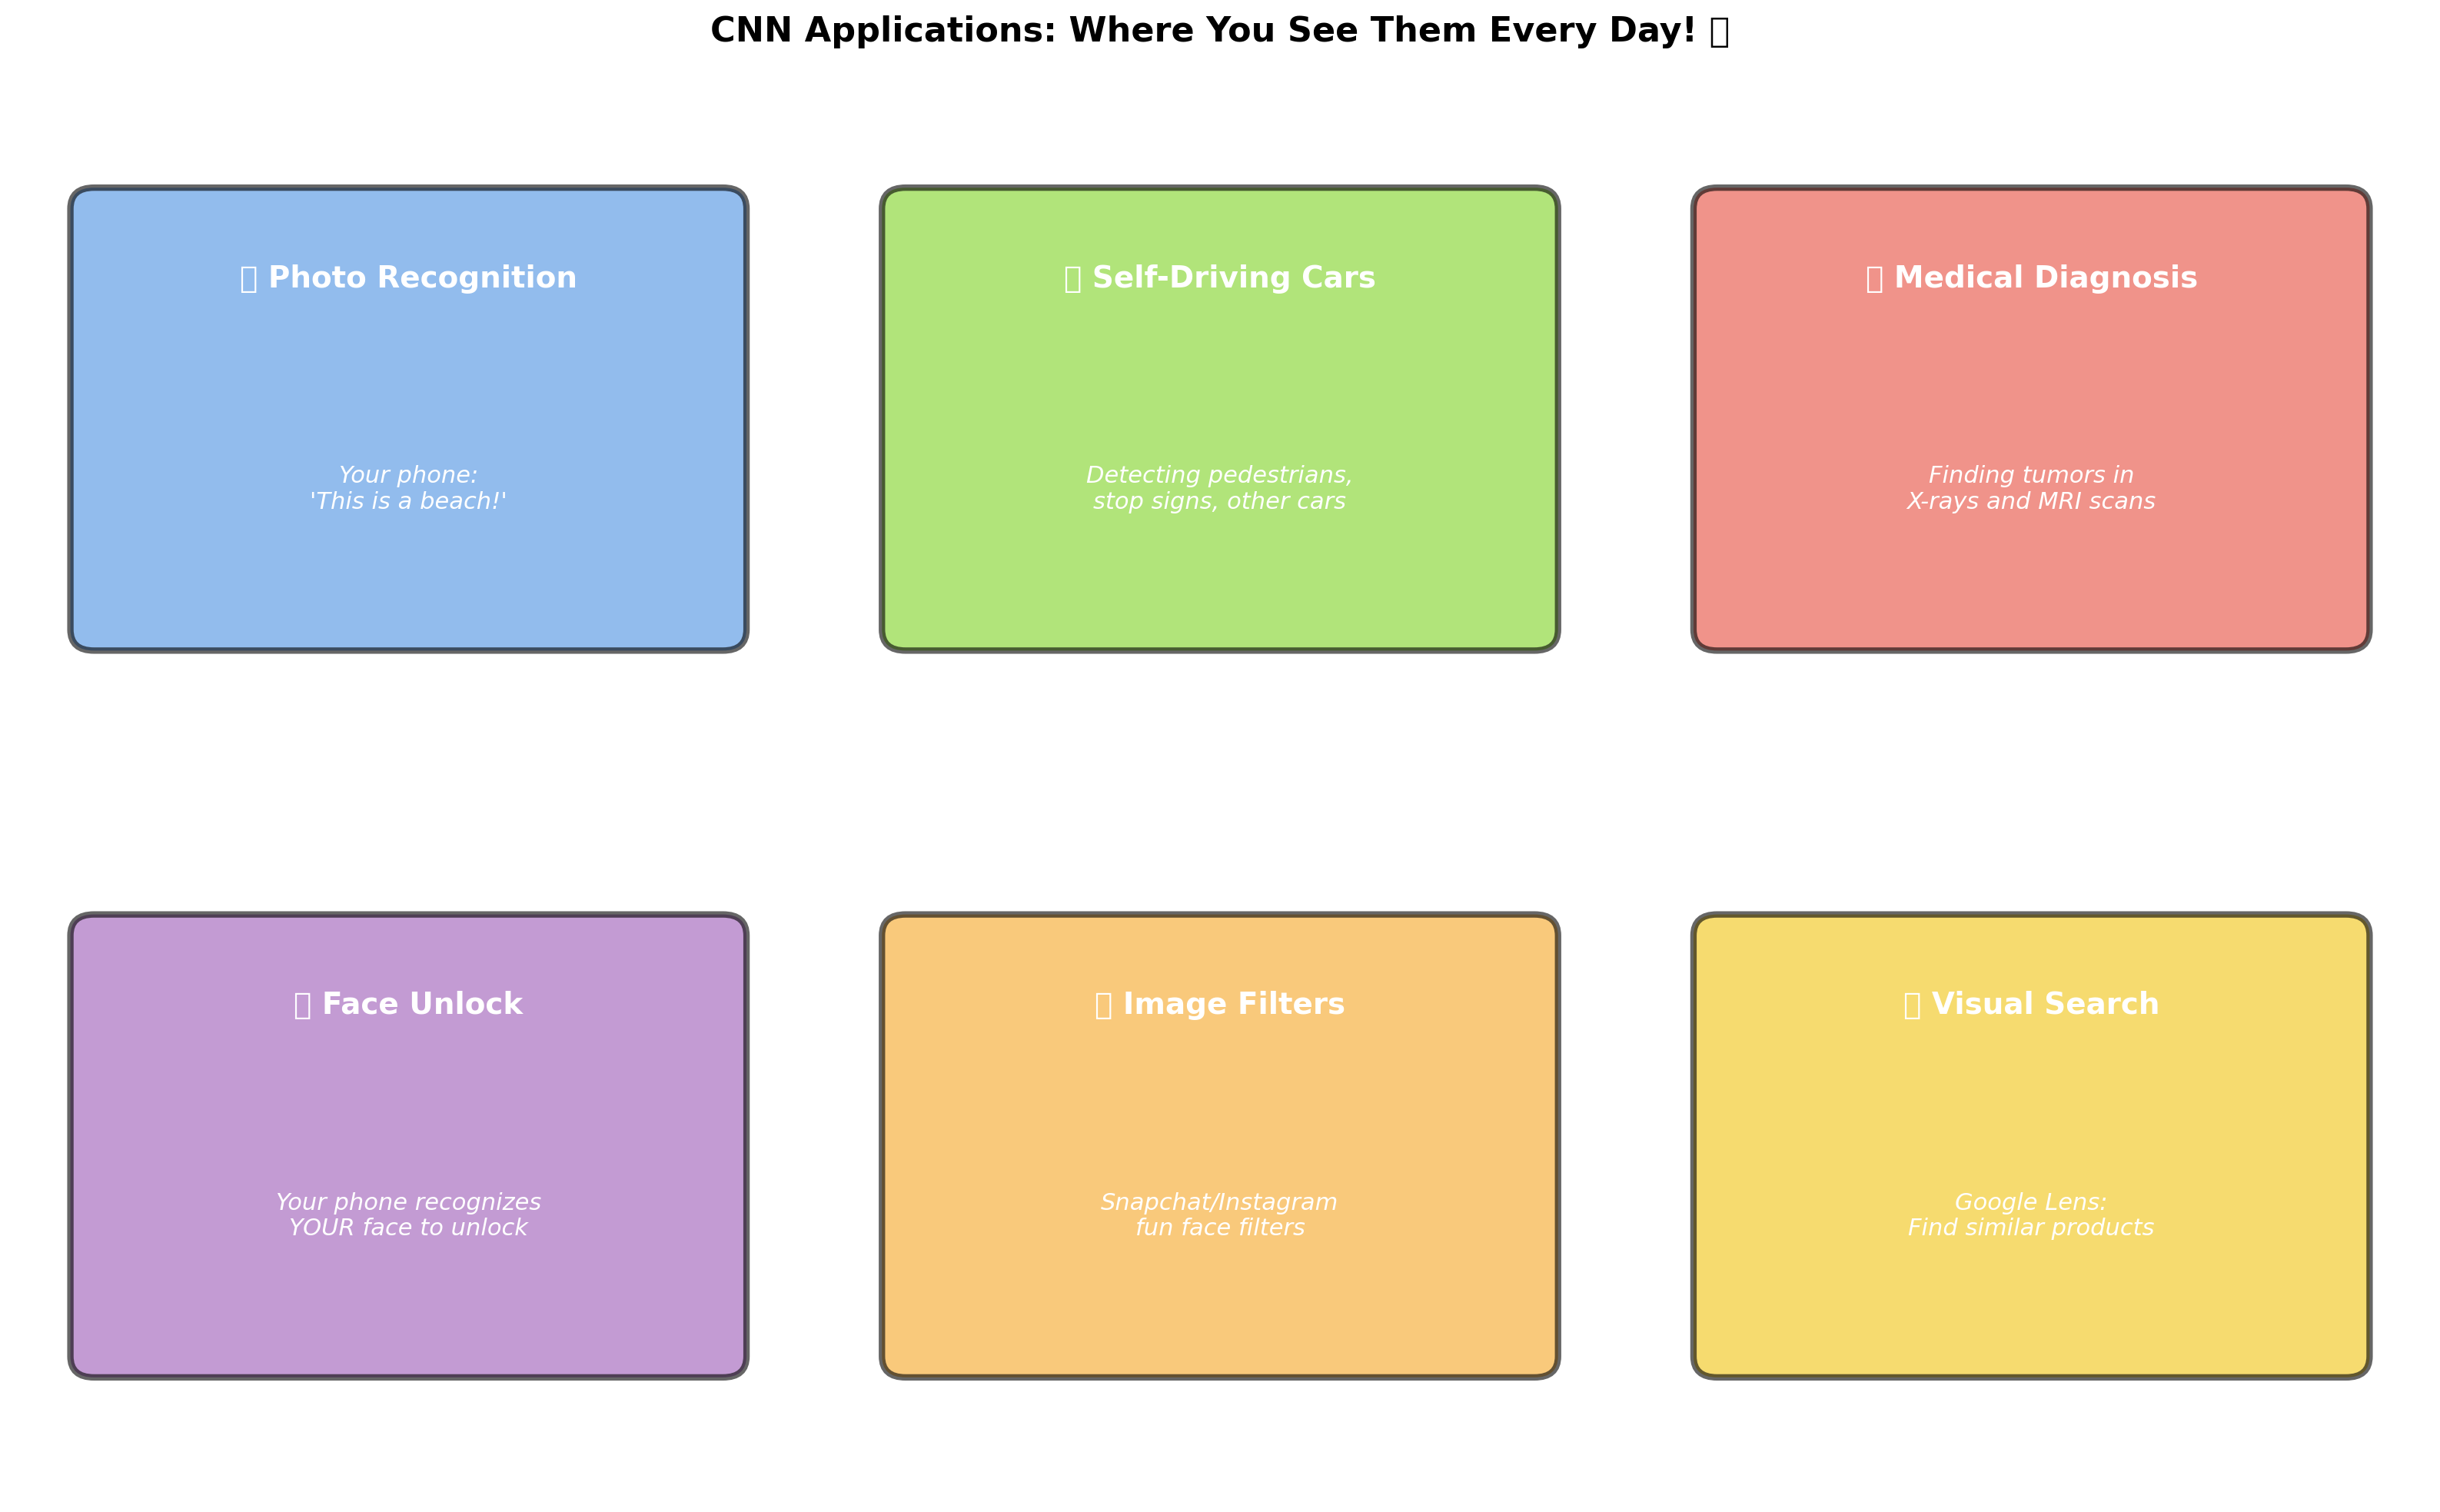
\includegraphics[width=0.85\textwidth]{../figures/cnn_applications.png}

\vspace{0.2cm}

\begin{alertblock}{Course Philosophy}
\textbf{Learn by seeing what's possible!} We'll focus on understanding what these networks can do and how to use them, not deriving complex mathematics.
\end{alertblock}
\end{frame}

% ========================================
% Section: Convolutional Neural Networks
% ========================================

\section{Convolutional Neural Networks (CNNs)}

\begin{frame}{CNNs: What Are They?}
\begin{columns}[t]
\begin{column}{0.48\textwidth}
\begin{block}{Simple Explanation}
\textbf{CNNs are neural networks designed for images.} They work by:
\begin{itemize}
\setlength{\itemsep}{2pt}
\item Looking at small patches of the image
\item Finding patterns (edges, shapes, textures)
\item Building up to complex objects
\item Making decisions based on what they see
\end{itemize}
\end{block}

\vspace{0.1cm}

\begin{exampleblock}{Why Not Regular NNs?}
\begin{itemize}
\setlength{\itemsep}{2pt}
\item Images have too many pixels
\item Spatial relationships matter
\item Same pattern appears in different places
\item CNNs are much more efficient
\end{itemize}
\end{exampleblock}
\end{column}

\begin{column}{0.48\textwidth}
\centering
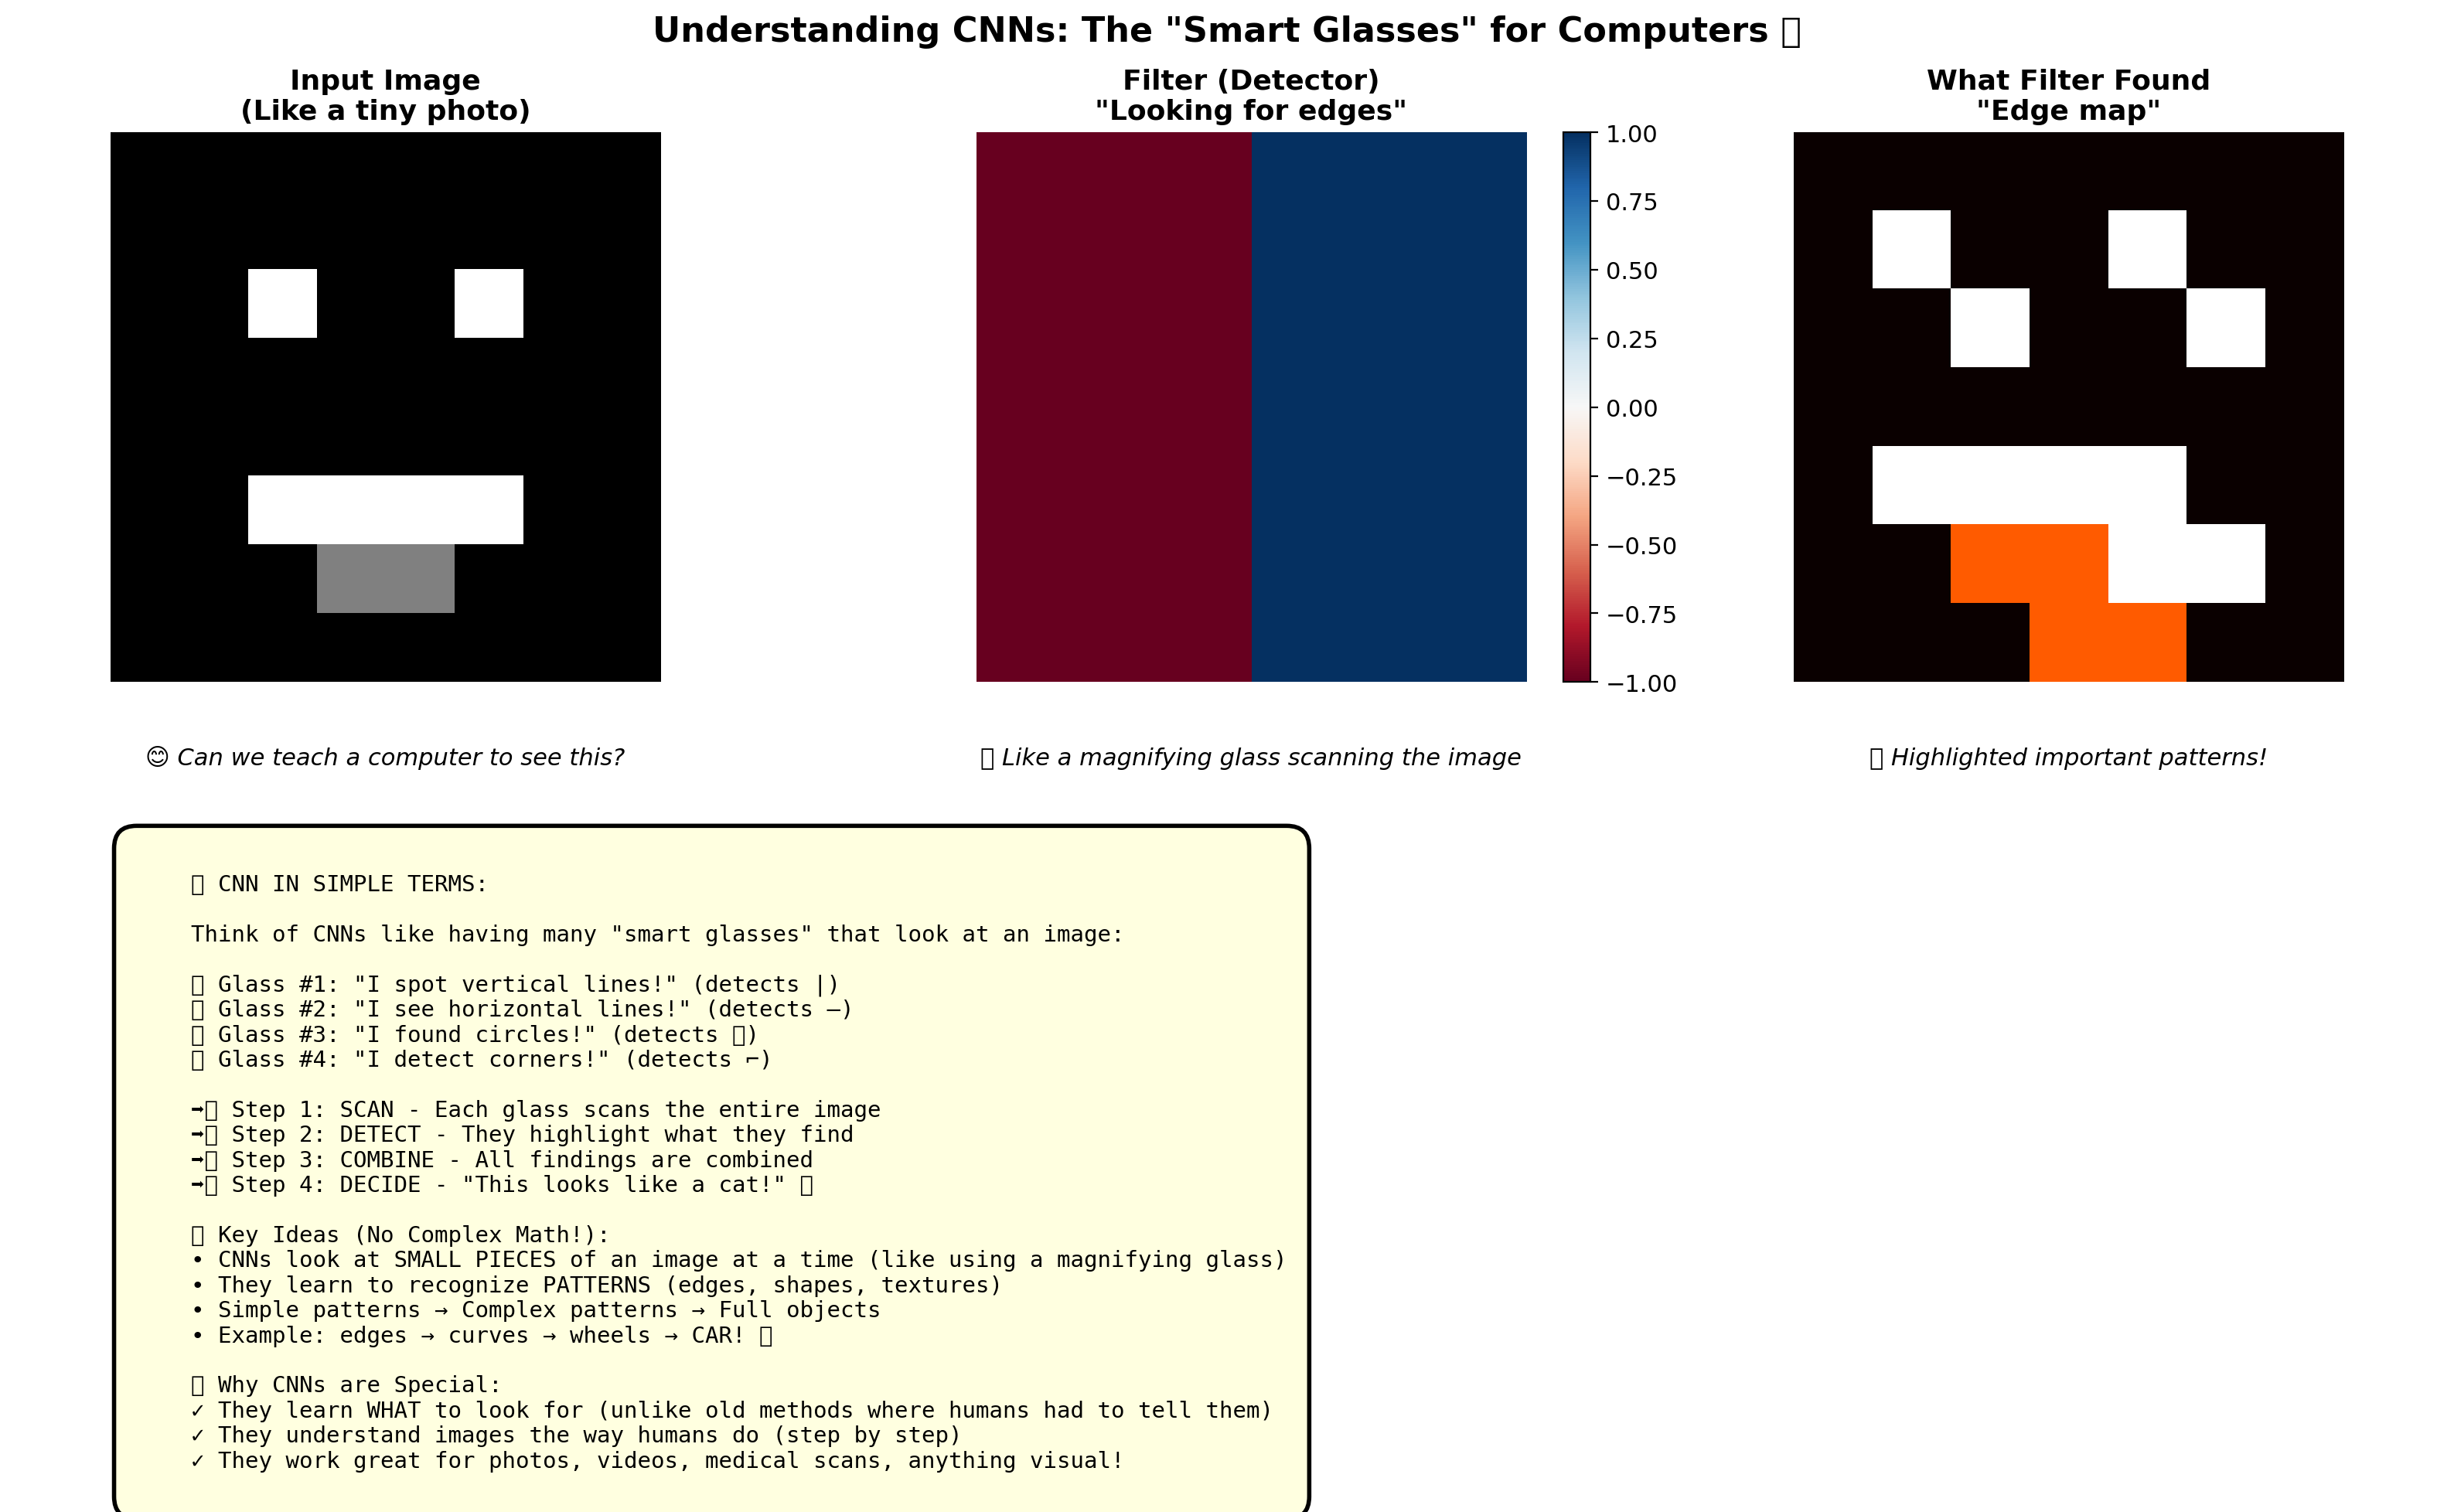
\includegraphics[width=\textwidth]{../figures/cnn_simple_intuition.png}

\vspace{0.15cm}

\begin{alertblock}{Key Insight}
CNNs learn to recognize patterns automatically - no manual feature engineering!
\end{alertblock}
\end{column}
\end{columns}
\end{frame}

\begin{frame}{How CNNs Process Images}
\centering
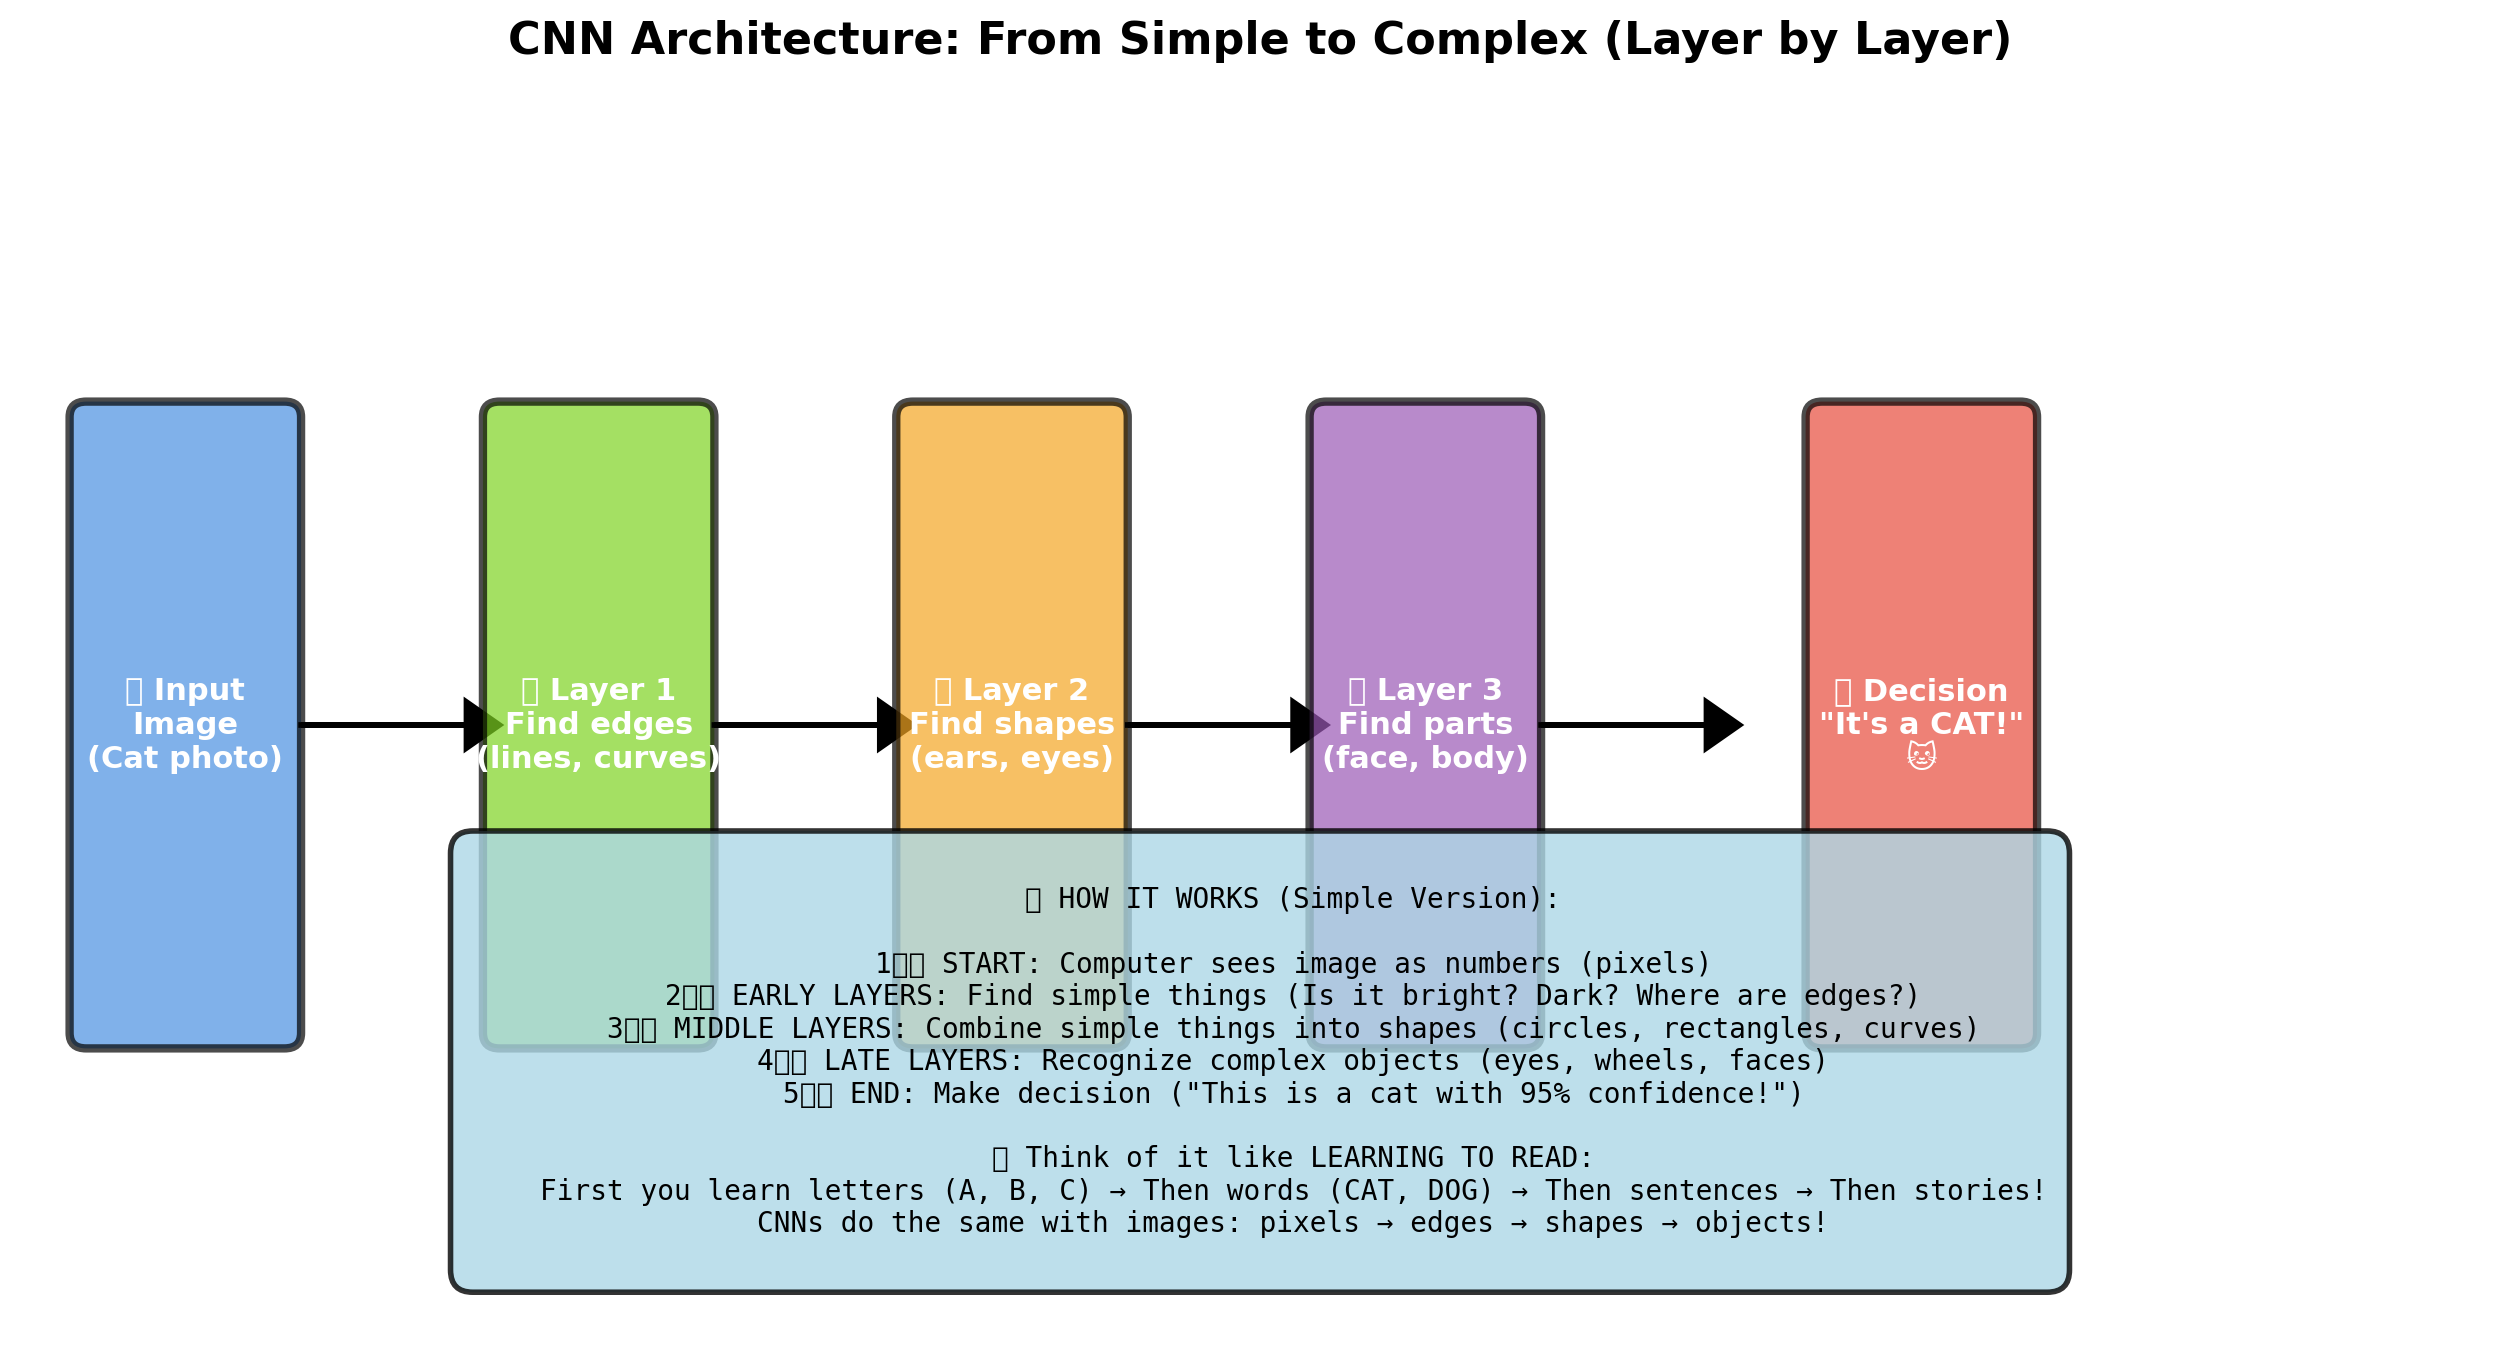
\includegraphics[width=0.9\textwidth]{../figures/cnn_simple_architecture.png}

\vspace{0.2cm}

\begin{block}{Processing Pipeline}
\textbf{Input Image} $\rightarrow$ \textbf{Find Edges} $\rightarrow$ \textbf{Find Shapes} $\rightarrow$ \textbf{Find Objects} $\rightarrow$ \textbf{Decision}
\end{block}

\begin{exampleblock}{Analogy}
Like how humans see: First we see lines and edges, then shapes, then we recognize "this is a cat!"
\end{exampleblock}
\end{frame}

\begin{frame}{CNNs vs Traditional Computer Vision}
\centering
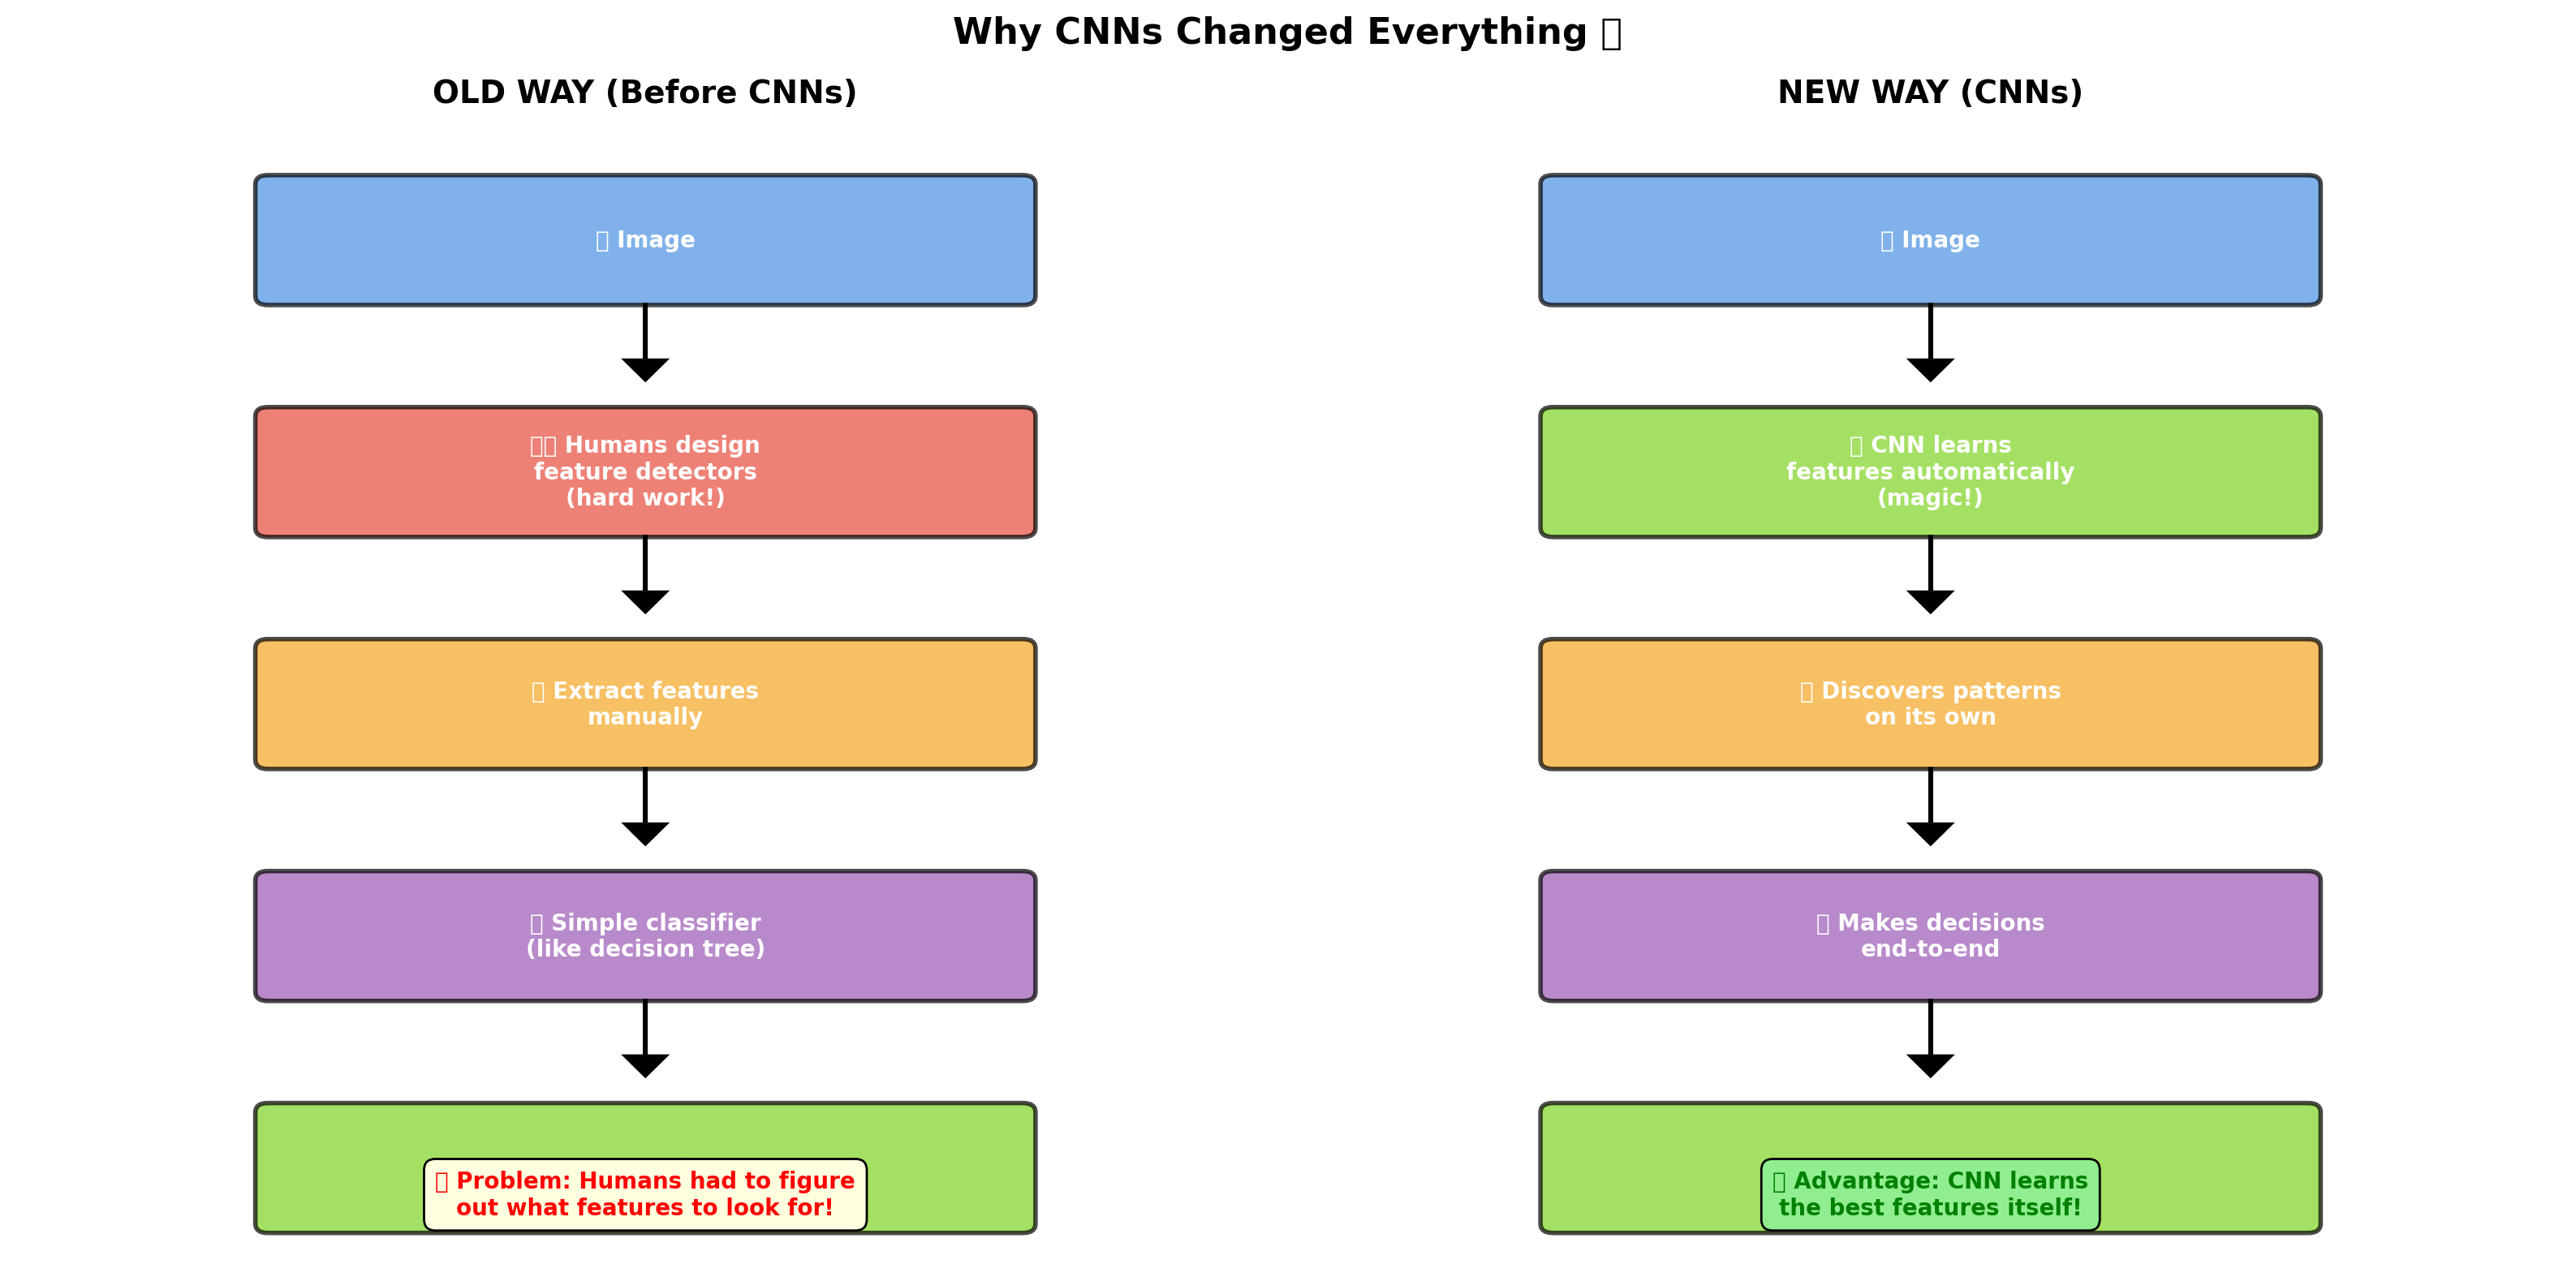
\includegraphics[width=0.85\textwidth]{../figures/cnn_vs_traditional.png}

\vspace{0.2cm}

\begin{columns}[t]
\begin{column}{0.48\textwidth}
\begin{block}{Traditional Methods}
\begin{itemize}
\setlength{\itemsep}{2pt}
\item Manual feature design
\item Hard to adapt to new tasks
\item Limited accuracy
\item Lots of expert knowledge needed
\end{itemize}
\end{block}
\end{column}

\begin{column}{0.48\textwidth}
\begin{exampleblock}{CNNs}
\begin{itemize}
\setlength{\itemsep}{2pt}
\item Automatic feature learning
\item Easily adapt to new problems
\item State-of-the-art accuracy
\item Just need training data
\end{itemize}
\end{exampleblock}
\end{column}
\end{columns}
\end{frame}

\begin{frame}{CNN Applications: Medical Imaging}
\begin{columns}[t]
\begin{column}{0.48\textwidth}
\begin{block}{Cancer Detection}
\textbf{Real Application:}
\begin{itemize}
\setlength{\itemsep}{2pt}
\item Detect tumors in X-rays and MRIs
\item Classify skin lesions (benign/malignant)
\item Analyze mammograms for breast cancer
\item Help radiologists work faster
\end{itemize}
\end{block}

\vspace{0.15cm}

\begin{exampleblock}{Impact}
\begin{itemize}
\setlength{\itemsep}{2pt}
\item Earlier disease detection
\item Fewer missed diagnoses
\item Reduced radiologist workload
\item Available in rural areas
\end{itemize}
\end{exampleblock}
\end{column}

\begin{column}{0.48\textwidth}
\begin{block}{Retinal Disease Diagnosis}
\textbf{Example: Google's Diabetic Retinopathy Detection}
\begin{itemize}
\setlength{\itemsep}{2pt}
\item Analyzes eye scans
\item Detects diabetes complications
\item Matches expert doctor accuracy
\item Used in India, Thailand
\end{itemize}
\end{block}

\vspace{0.15cm}

\begin{alertblock}{Success Story}
FDA-approved AI systems now assist doctors in real hospitals!
\end{alertblock}
\end{column}
\end{columns}
\end{frame}

\begin{frame}{CNN Applications: Self-Driving Cars}
\begin{columns}[t]
\begin{column}{0.48\textwidth}
\begin{block}{Lane Detection}
\textbf{What CNNs Do:}
\begin{itemize}
\setlength{\itemsep}{2pt}
\item Identify road lane markings
\item Track lane boundaries in real-time
\item Work in various lighting conditions
\item Handle curves and intersections
\end{itemize}
\end{block}

\vspace{0.1cm}

\begin{block}{Object Detection}
\begin{itemize}
\setlength{\itemsep}{2pt}
\item Detect pedestrians, cars, cyclists
\item Recognize traffic signs and lights
\item Estimate distance to objects
\item Predict object movement
\end{itemize}
\end{block}
\end{column}

\begin{column}{0.48\textwidth}
\begin{exampleblock}{Companies Using This}
\begin{itemize}
\setlength{\itemsep}{2pt}
\item \textbf{Tesla:} Full Self-Driving (FSD)
\item \textbf{Waymo:} Autonomous taxis
\item \textbf{Cruise:} Robotaxis in SF
\item \textbf{Mobileye:} Driver assistance
\end{itemize}
\end{exampleblock}

\vspace{0.15cm}

\begin{alertblock}{Real Deployment}
Over 1 million vehicles use CNN-based vision systems today!
\end{alertblock}
\end{column}
\end{columns}
\end{frame}

\begin{frame}{CNN Applications: Face Recognition}
\begin{columns}[t]
\begin{column}{0.48\textwidth}
\begin{block}{Phone Unlock (Face ID)}
\textbf{How It Works:}
\begin{itemize}
\setlength{\itemsep}{2pt}
\item CNN extracts facial features
\item Creates unique "face print"
\item Compares to stored template
\item Works in different lighting
\item Adapts to appearance changes
\end{itemize}
\end{block}

\vspace{0.15cm}

\begin{exampleblock}{Daily Use Cases}
\begin{itemize}
\setlength{\itemsep}{2pt}
\item iPhone/Android face unlock
\item Photo organization (Google Photos)
\item Security access control
\item Airport immigration
\end{itemize}
\end{exampleblock}
\end{column}

\begin{column}{0.48\textwidth}
\begin{block}{Social Media Applications}
\begin{itemize}
\setlength{\itemsep}{2pt}
\item \textbf{Facebook:} Auto-tag friends in photos
\item \textbf{Snapchat:} Face filters and effects
\item \textbf{Instagram:} Beauty filters
\item \textbf{TikTok:} Face tracking for AR
\end{itemize}
\end{block}

\vspace{0.15cm}

\begin{alertblock}{Privacy Note}
Face recognition raises important privacy concerns - always consider ethics!
\end{alertblock}
\end{column}
\end{columns}
\end{frame}

\begin{frame}{CNN Applications: Security \& Surveillance}
\begin{columns}[t]
\begin{column}{0.48\textwidth}
\begin{block}{Smart Security Cameras}
\textbf{Capabilities:}
\begin{itemize}
\setlength{\itemsep}{2pt}
\item Detect people vs animals
\item Recognize package delivery
\item Identify suspicious behavior
\item Track movement patterns
\item Send targeted alerts
\end{itemize}
\end{block}

\vspace{0.15cm}

\begin{exampleblock}{Consumer Products}
\begin{itemize}
\setlength{\itemsep}{2pt}
\item Ring Doorbell cameras
\item Nest security systems
\item Arlo smart cameras
\item Reduce false alarms by 90\%
\end{itemize}
\end{exampleblock}
\end{column}

\begin{column}{0.48\textwidth}
\begin{block}{Retail Applications}
\textbf{Amazon Go Stores:}
\begin{itemize}
\setlength{\itemsep}{2pt}
\item Track what customers pick up
\item Automatic checkout (no cashiers)
\item Prevent shoplifting
\item Analyze shopping behavior
\end{itemize}
\end{block}

\vspace{0.15cm}

\begin{alertblock}{Industry Impact}
Checkout-free stores save 75\% of labor costs while improving customer experience!
\end{alertblock}
\end{column}
\end{columns}
\end{frame}

\begin{frame}{CNN Applications: Satellite Imagery Analysis}
\begin{columns}[t]
\begin{column}{0.48\textwidth}
\begin{block}{Environmental Monitoring}
\textbf{Applications:}
\begin{itemize}
\setlength{\itemsep}{2pt}
\item Track deforestation in Amazon
\item Monitor crop health
\item Detect illegal fishing
\item Assess disaster damage
\item Map urban growth
\end{itemize}
\end{block}

\vspace{0.15cm}

\begin{exampleblock}{Real Projects}
\begin{itemize}
\setlength{\itemsep}{2pt}
\item \textbf{Planet Labs:} Daily Earth imaging
\item \textbf{Global Fishing Watch:} Ocean monitoring
\item \textbf{NASA:} Climate change tracking
\end{itemize}
\end{exampleblock}
\end{column}

\begin{column}{0.48\textwidth}
\begin{block}{Humanitarian Uses}
\begin{itemize}
\setlength{\itemsep}{2pt}
\item Count refugees in camps
\item Assess natural disaster impact
\item Map poverty indicators
\item Monitor conflict zones
\item Guide relief efforts
\end{itemize}
\end{block}

\vspace{0.15cm}

\begin{alertblock}{Scale}
CNNs can analyze millions of satellite images - impossible for humans alone!
\end{alertblock}
\end{column}
\end{columns}
\end{frame}

% ========================================
% Section: Generative Models Overview
% ========================================

\section{Generative Models: Creating New Content}

\begin{frame}{What Are Generative Models?}
\centering
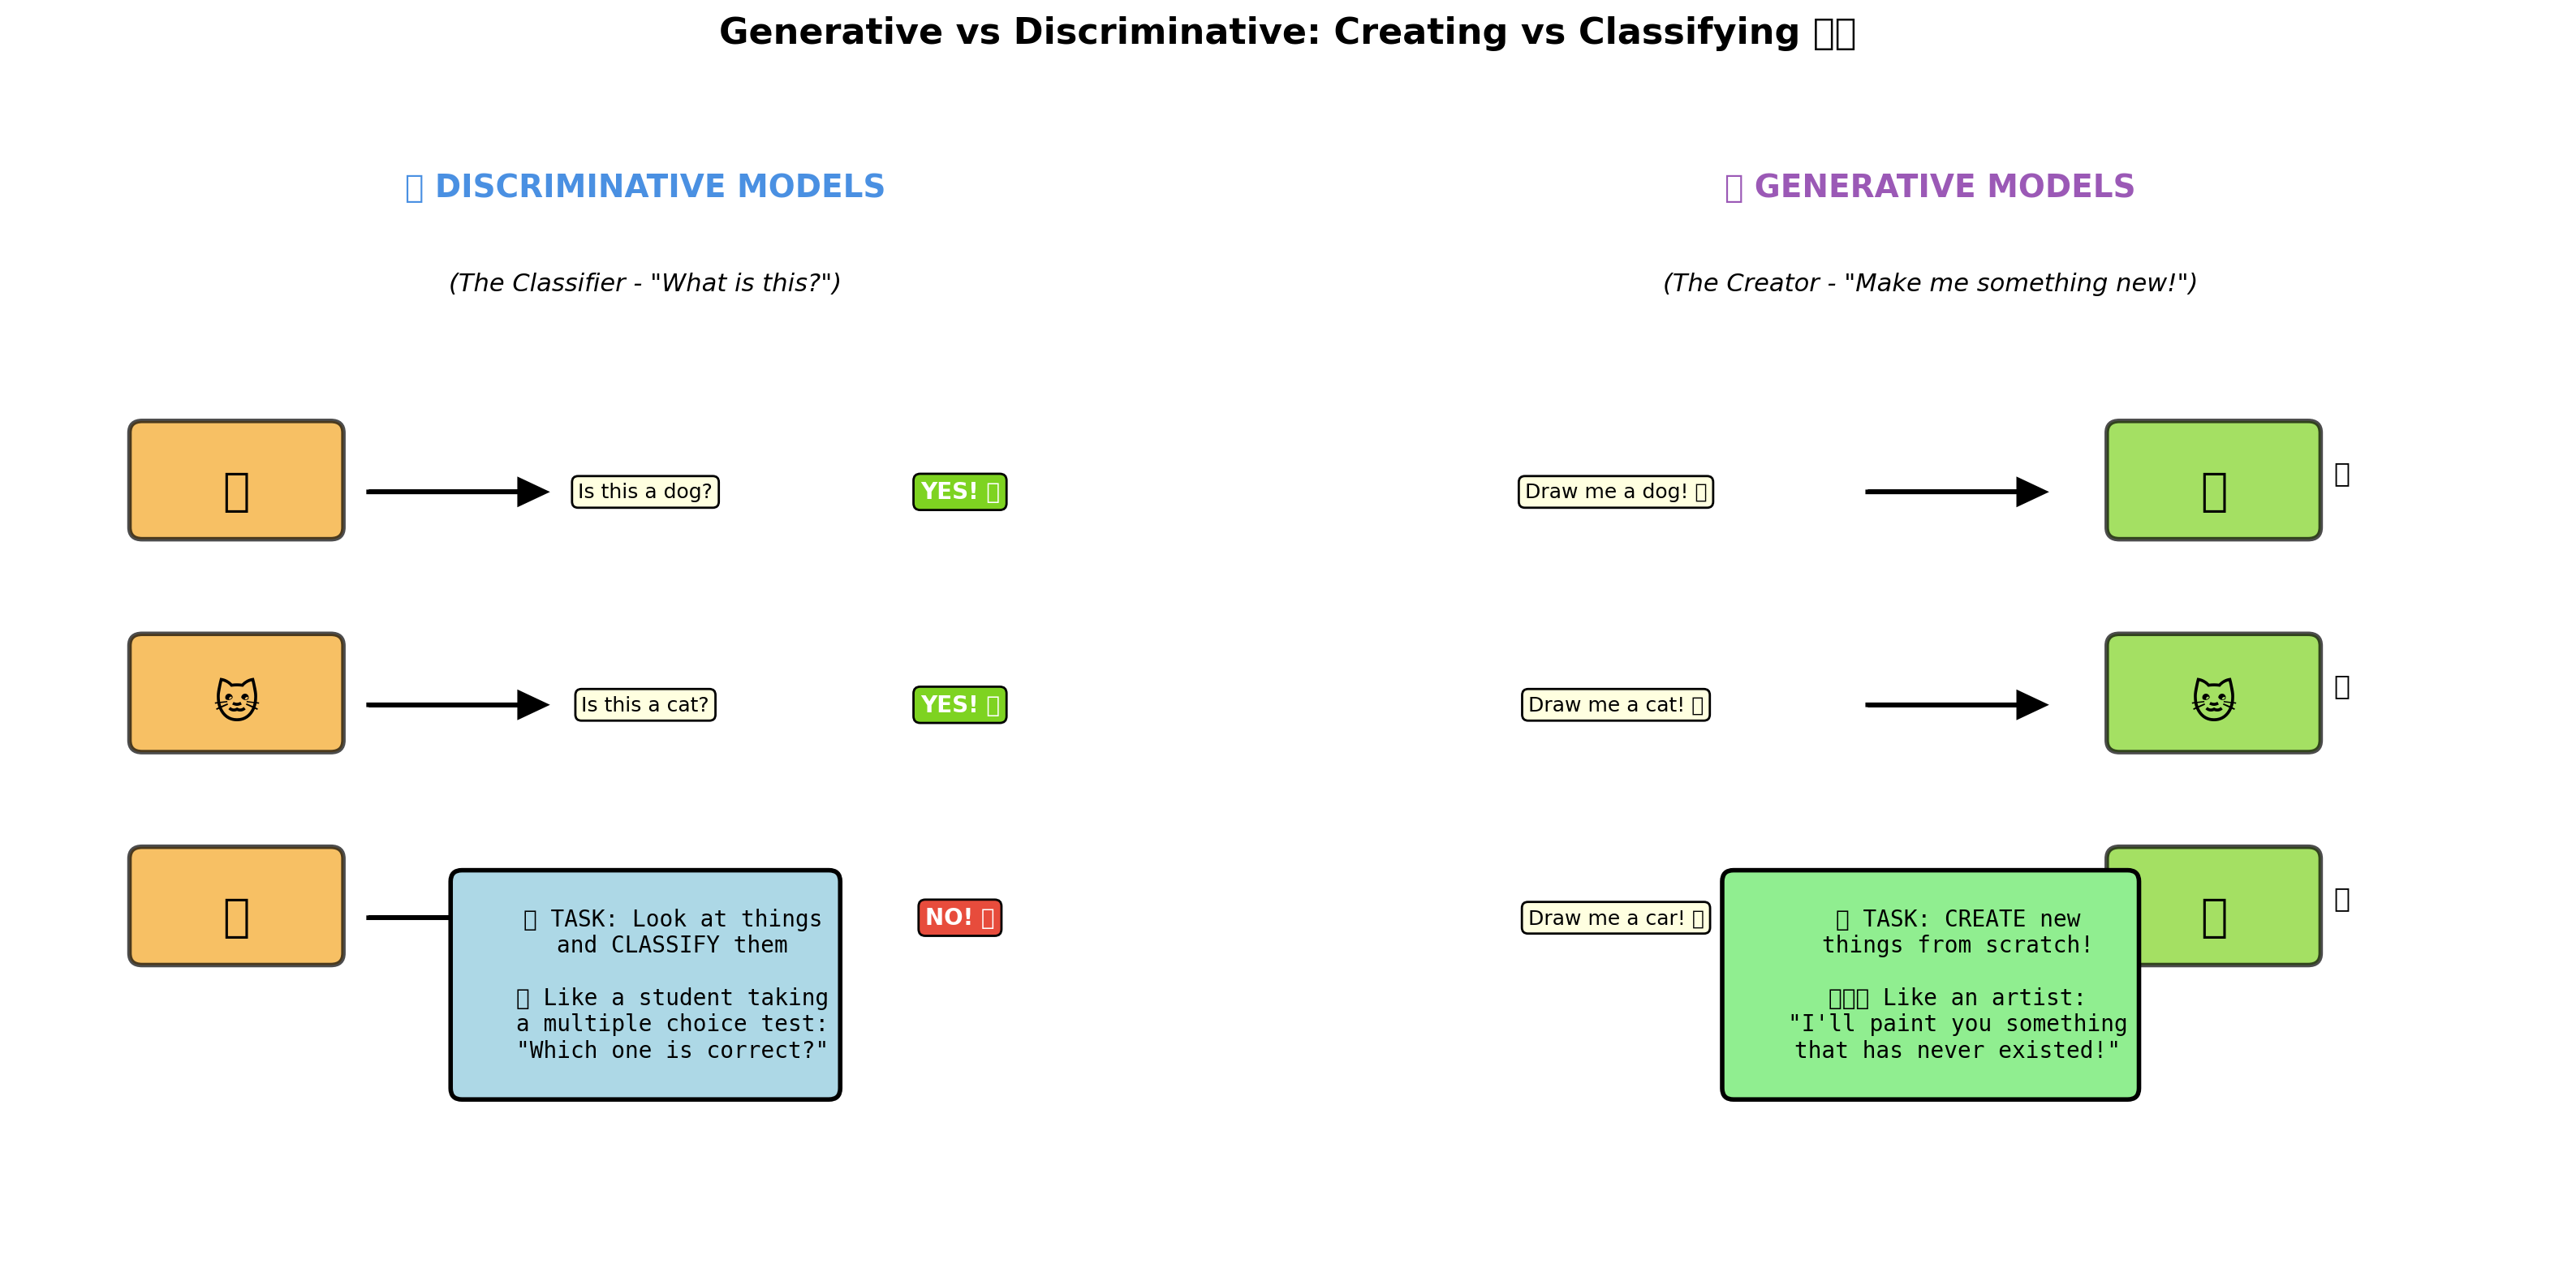
\includegraphics[width=0.85\textwidth]{../figures/generative_vs_discriminative.png}

\vspace{0.2cm}

\begin{columns}[t]
\begin{column}{0.48\textwidth}
\begin{block}{Discriminative Models}
\textbf{What they do:}
\begin{itemize}
\setlength{\itemsep}{2pt}
\item Classify/label existing data
\item "Is this a cat or dog?"
\item CNNs for image classification
\end{itemize}
\end{block}
\end{column}

\begin{column}{0.48\textwidth}
\begin{exampleblock}{Generative Models}
\textbf{What they do:}
\begin{itemize}
\setlength{\itemsep}{2pt}
\item Create new data
\item "Generate a new cat image"
\item GANs, VAEs, Diffusion models
\end{itemize}
\end{exampleblock}
\end{column}
\end{columns}
\end{frame}

\begin{frame}{Generative Model Applications Overview}
\centering
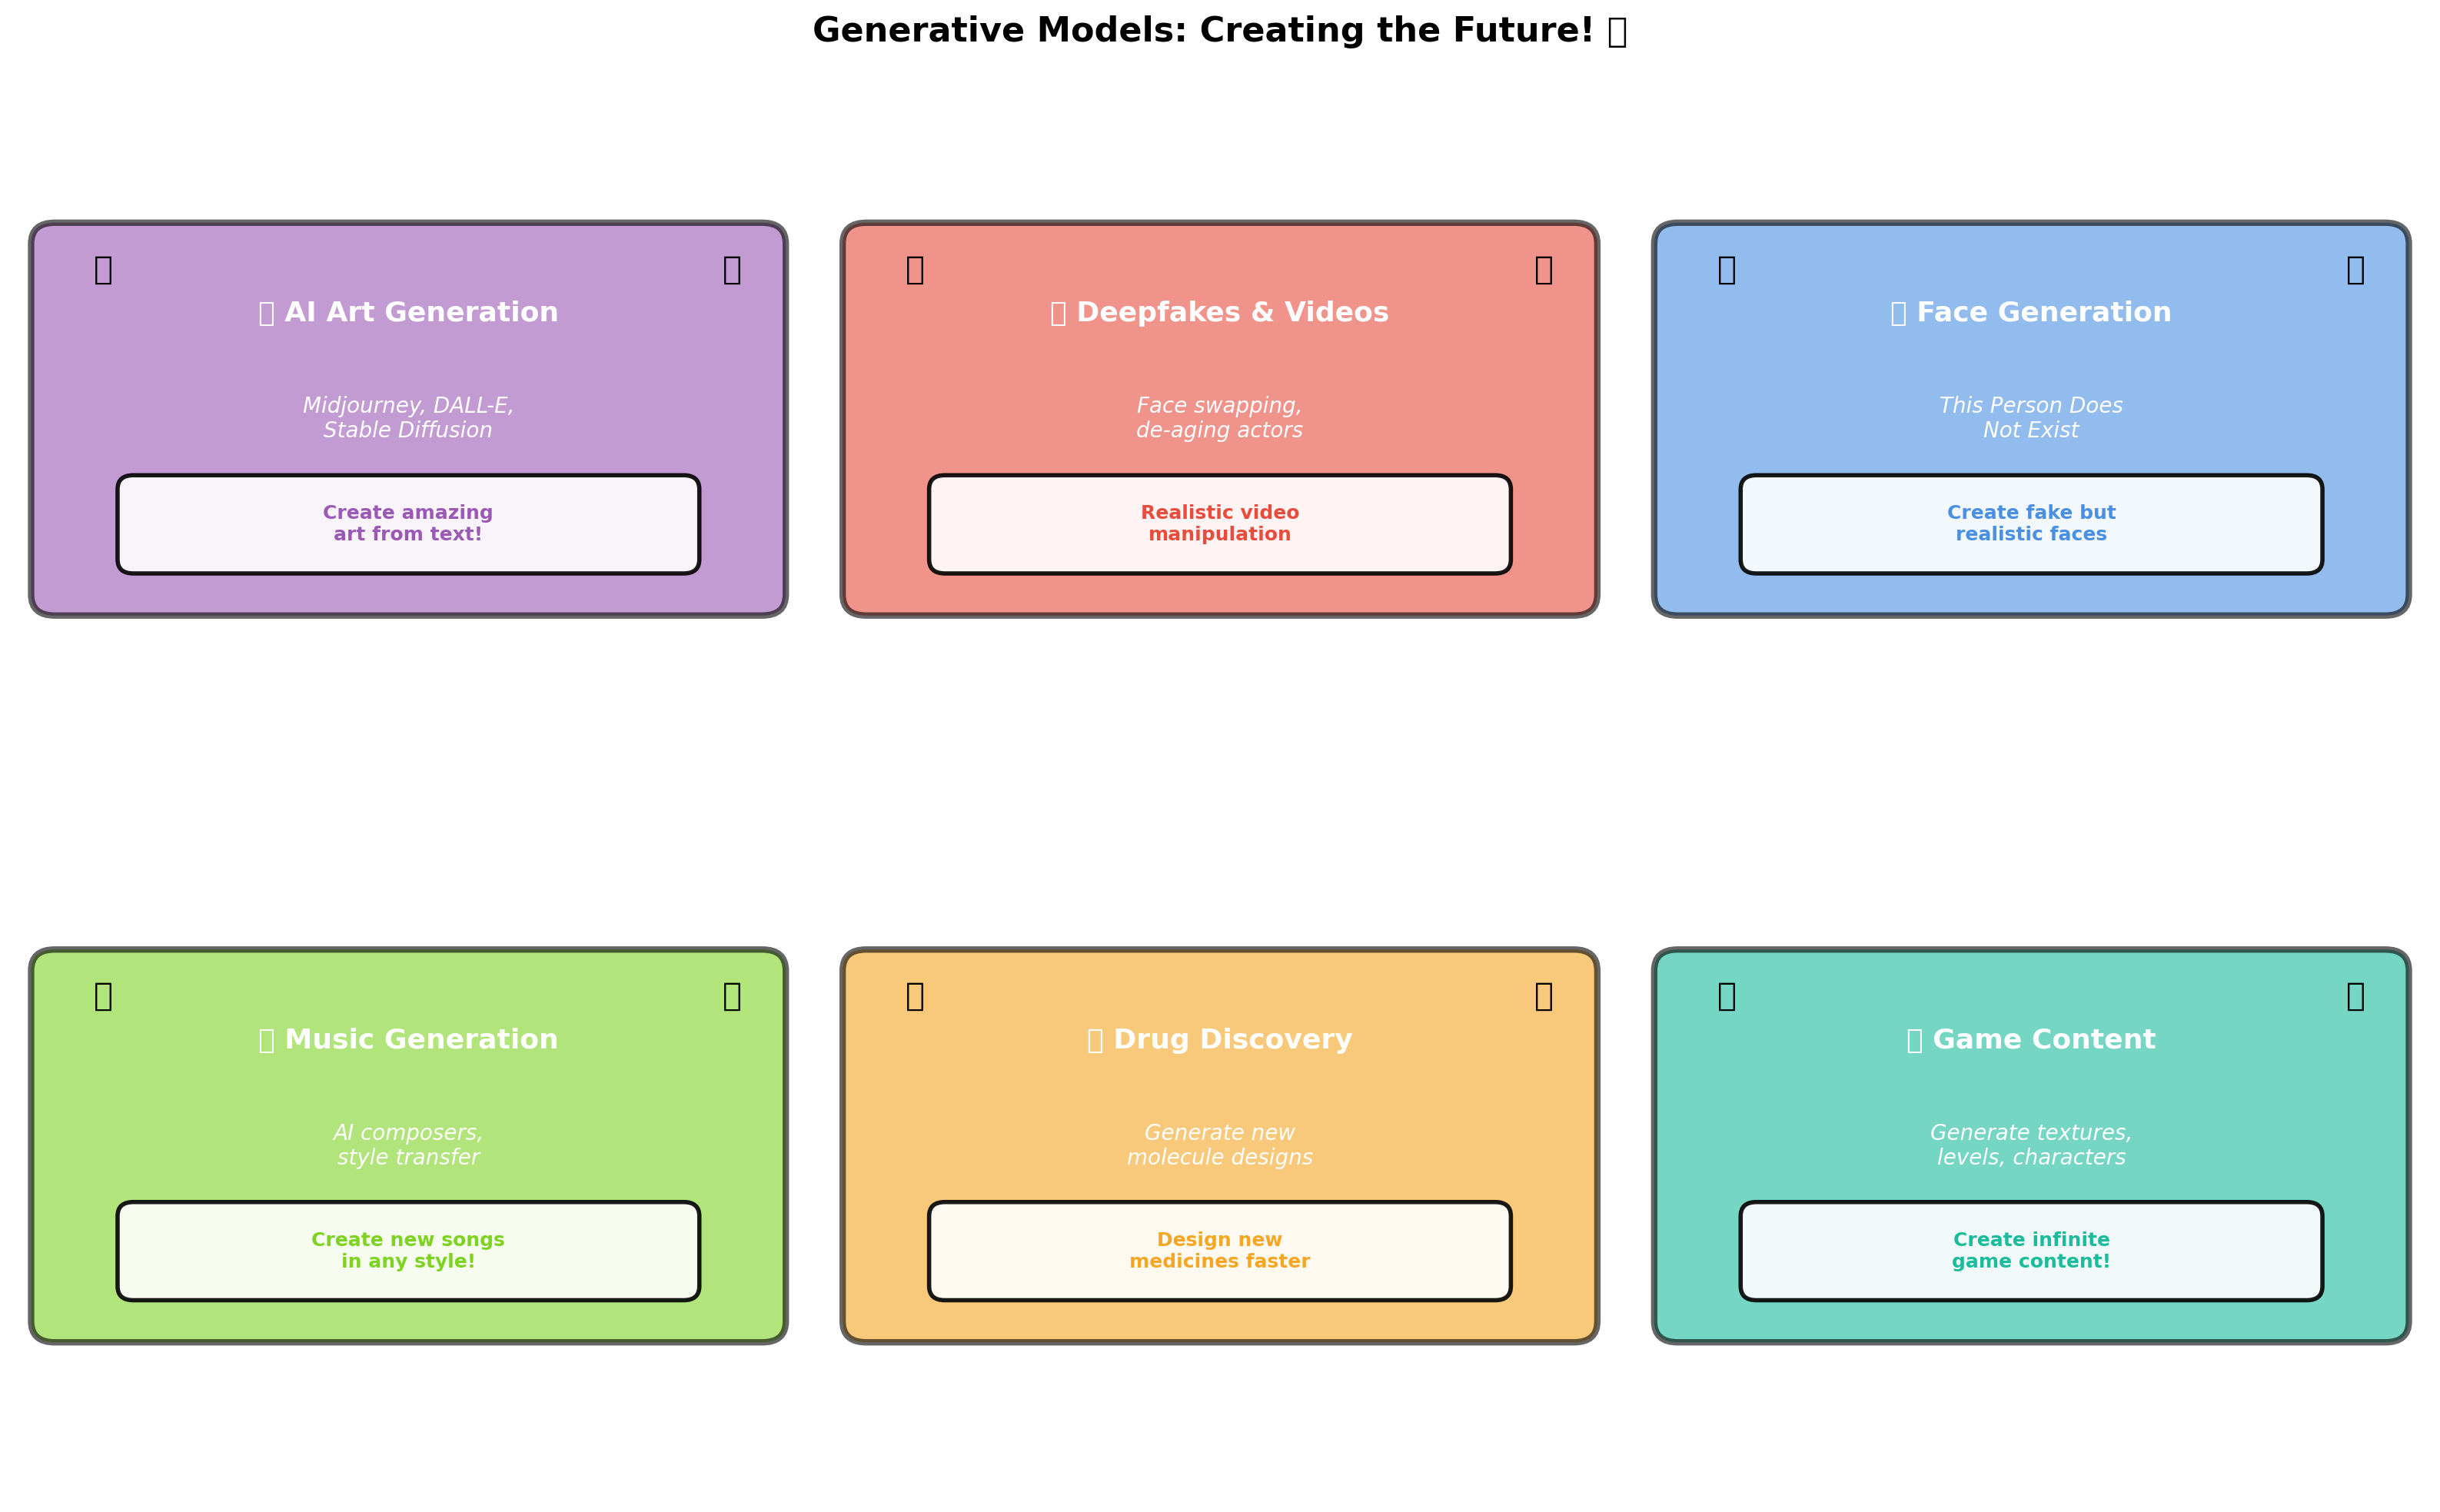
\includegraphics[width=0.88\textwidth]{../figures/generative_applications.png}

\vspace{0.2cm}

\begin{alertblock}{Three Main Types We'll Cover}
\begin{enumerate}
\item \textbf{GANs (Generative Adversarial Networks):} Two networks compete to create realistic images
\item \textbf{VAEs (Variational Autoencoders):} Learn compressed representations, generate variations
\item \textbf{Diffusion Models:} Start with noise, gradually create detailed images
\end{enumerate}
\end{alertblock}
\end{frame}

% ========================================
% Section: GANs
% ========================================

\section{GANs: Generative Adversarial Networks}

\begin{frame}{GANs: The Basic Idea}
\centering
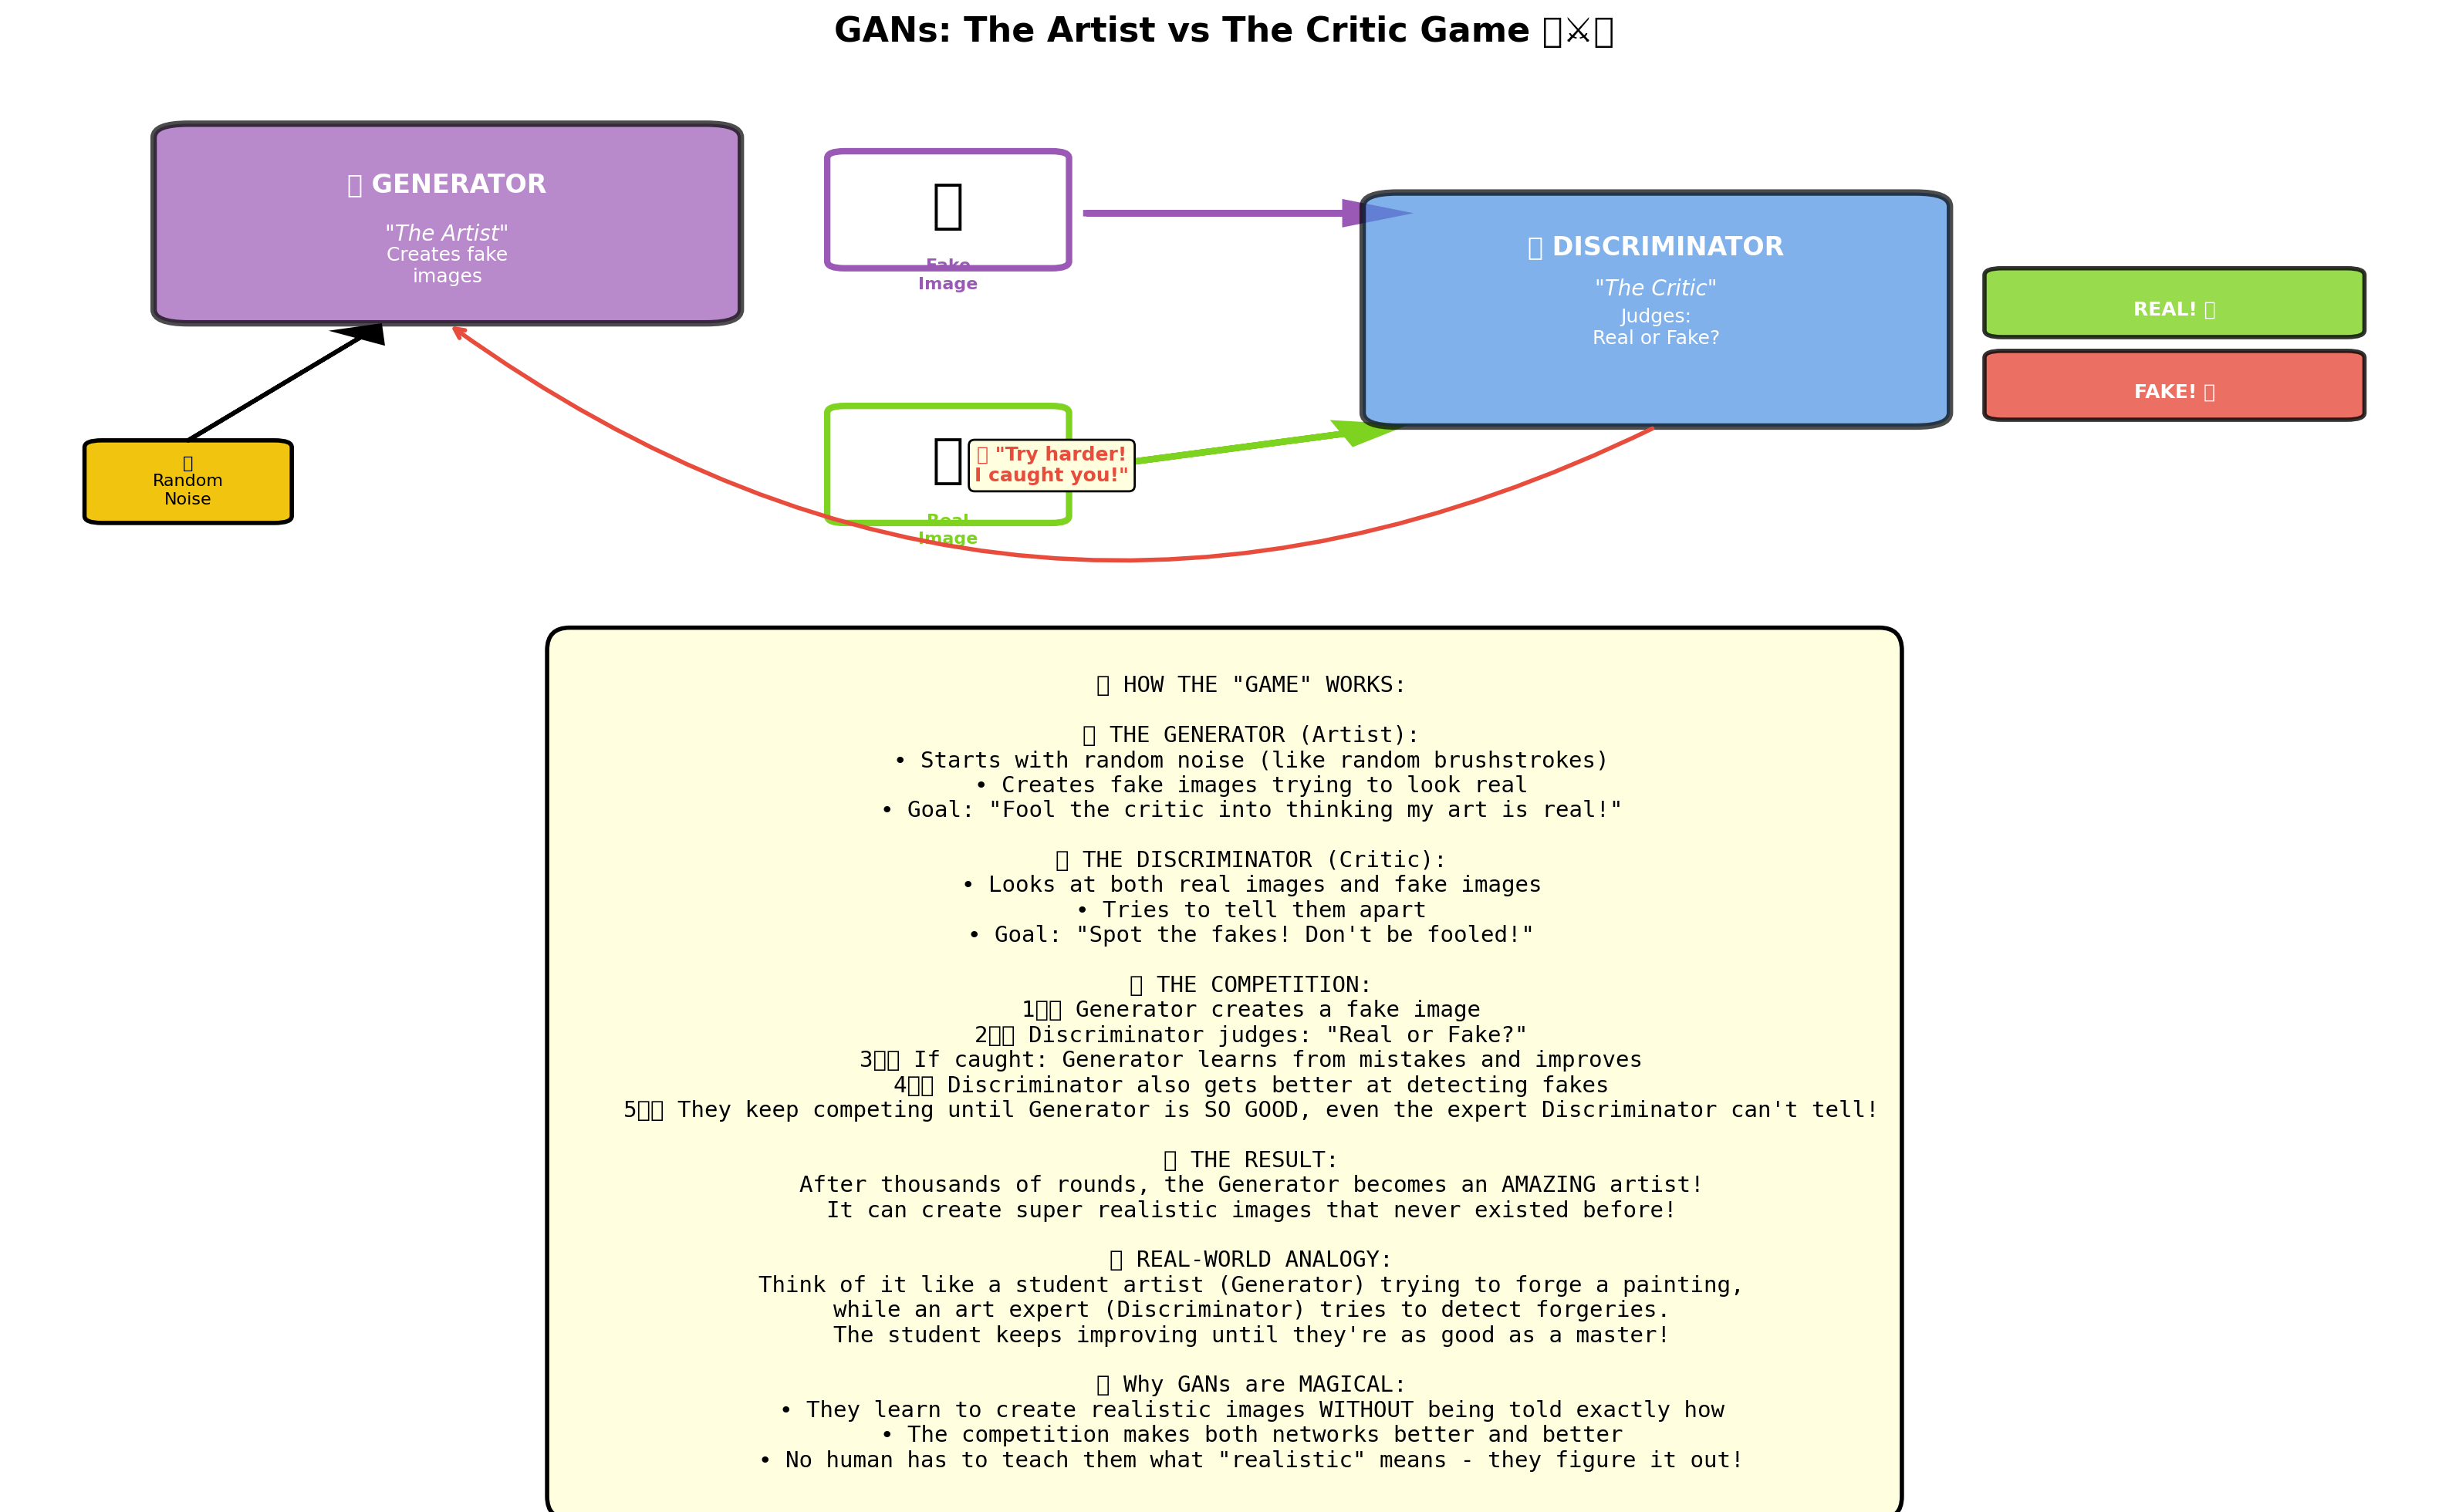
\includegraphics[width=0.85\textwidth]{../figures/gan_simple_concept.png}

\vspace{0.2cm}

\begin{block}{Simple Explanation}
\textbf{Two neural networks compete:}
\begin{itemize}
\setlength{\itemsep}{3pt}
\item \textbf{Generator:} Creates fake images (like an art forger)
\item \textbf{Discriminator:} Tries to spot fakes (like an art detective)
\item They get better by competing with each other
\item Eventually, fakes become indistinguishable from real!
\end{itemize}
\end{block}
\end{frame}

\begin{frame}{GAN Application: AI Art Generation}
\begin{columns}[t]
\begin{column}{0.48\textwidth}
\begin{block}{Artbreeder}
\textbf{What it does:}
\begin{itemize}
\setlength{\itemsep}{2pt}
\item Generate unique portraits
\item Mix different faces together
\item Adjust age, gender, ethnicity
\item Create landscapes, album covers
\item Used by 10+ million users
\end{itemize}
\end{block}

\vspace{0.15cm}

\begin{exampleblock}{How Artists Use It}
\begin{itemize}
\setlength{\itemsep}{2pt}
\item Book cover illustrations
\item Character design for games
\item Concept art for films
\item Social media content
\end{itemize}
\end{exampleblock}
\end{column}

\begin{column}{0.48\textwidth}
\begin{block}{ThisPersonDoesNotExist.com}
\begin{itemize}
\setlength{\itemsep}{2pt}
\item Generates random faces
\item 100\% synthetic people
\item Photorealistic quality
\item New face every refresh
\item Built with StyleGAN
\end{itemize}
\end{block}

\vspace{0.15cm}

\begin{alertblock}{Try It Yourself!}
Visit the website - every face you see was created by AI, not a photo!
\end{alertblock}
\end{column}
\end{columns}
\end{frame}

\begin{frame}{GAN Application: Deepfake Detection}
\begin{columns}[t]
\begin{column}{0.48\textwidth}
\begin{block}{The Problem}
\textbf{Malicious Uses:}
\begin{itemize}
\setlength{\itemsep}{2pt}
\item Fake celebrity videos
\item Misinformation campaigns
\item Identity fraud
\item Non-consensual content
\end{itemize}
\end{block}

\vspace{0.15cm}

\begin{exampleblock}{The Solution}
\textbf{GANs fight GANs:}
\begin{itemize}
\setlength{\itemsep}{2pt}
\item Train detectors on fake data
\item Identify artifacts and inconsistencies
\item Real-time video verification
\item Protect public figures
\end{itemize}
\end{exampleblock}
\end{column}

\begin{column}{0.48\textwidth}
\begin{block}{Real Deployments}
\begin{itemize}
\setlength{\itemsep}{2pt}
\item \textbf{Facebook/Meta:} Deepfake detection system
\item \textbf{Microsoft:} Video Authenticator tool
\item \textbf{Intel:} FakeCatcher (96\% accuracy)
\item \textbf{Adobe:} Content Authenticity Initiative
\end{itemize}
\end{block}

\vspace{0.15cm}

\begin{alertblock}{Arms Race}
Detection technology must constantly evolve as GANs improve!
\end{alertblock}
\end{column}
\end{columns}
\end{frame}

\begin{frame}{GAN Application: Synthetic Medical Data}
\begin{columns}[t]
\begin{column}{0.48\textwidth}
\begin{block}{Why Generate Medical Data?}
\textbf{Privacy \& Scarcity Issues:}
\begin{itemize}
\setlength{\itemsep}{2pt}
\item Real patient data is private (HIPAA)
\item Rare diseases lack training samples
\item Hard to share data between hospitals
\item Need diverse examples for AI training
\end{itemize}
\end{block}

\vspace{0.15cm}

\begin{exampleblock}{What GANs Generate}
\begin{itemize}
\setlength{\itemsep}{2pt}
\item Synthetic X-rays
\item Artificial MRI scans
\item Fake patient records
\item Privacy-preserving datasets
\end{itemize}
\end{exampleblock}
\end{column}

\begin{column}{0.48\textwidth}
\begin{block}{Real Research Applications}
\begin{itemize}
\setlength{\itemsep}{2pt}
\item \textbf{Mayo Clinic:} Generate rare tumor samples
\item \textbf{Stanford:} Synthetic chest X-rays
\item \textbf{MIT:} Privacy-safe medical records
\item Train better AI without compromising privacy
\end{itemize}
\end{block}

\vspace{0.15cm}

\begin{alertblock}{Impact}
Enables medical AI research while protecting patient privacy!
\end{alertblock}
\end{column}
\end{columns}
\end{frame}

\begin{frame}{GAN Application: Game Character Creation}
\begin{columns}[t]
\begin{column}{0.48\textwidth}
\begin{block}{Modern Game Development}
\textbf{How GANs Help:}
\begin{itemize}
\setlength{\itemsep}{2pt}
\item Generate unique NPC faces
\item Create diverse character variations
\item Design textures and materials
\item Procedural content generation
\item Speed up asset creation
\end{itemize}
\end{block}

\vspace{0.15cm}

\begin{exampleblock}{Real Game Studios}
\begin{itemize}
\setlength{\itemsep}{2pt}
\item \textbf{EA Sports:} Generate realistic player faces
\item \textbf{Ubisoft:} NPC diversity in Assassin's Creed
\item Reduce manual art time by 70\%
\end{itemize}
\end{exampleblock}
\end{column}

\begin{column}{0.48\textwidth}
\begin{block}{Player Customization}
\begin{itemize}
\setlength{\itemsep}{2pt}
\item Infinite character appearance options
\item Realistic face generation
\item Upload photo for custom avatar
\item AI-assisted character design
\end{itemize}
\end{block}

\vspace{0.15cm}

\begin{alertblock}{Industry Adoption}
Major game engines (Unity, Unreal) now integrate GAN-based tools!
\end{alertblock}
\end{column}
\end{columns}
\end{frame}

\begin{frame}{GAN Application: Fashion Design}
\begin{columns}[t]
\begin{column}{0.48\textwidth}
\begin{block}{AI Fashion Designers}
\textbf{What They Generate:}
\begin{itemize}
\setlength{\itemsep}{2pt}
\item New clothing designs
\item Pattern and texture variations
\item Color scheme combinations
\item Style transfer between eras
\item Personalized recommendations
\end{itemize}
\end{block}

\vspace{0.15cm}

\begin{exampleblock}{Fashion Companies Using AI}
\begin{itemize}
\setlength{\itemsep}{2pt}
\item \textbf{Stitch Fix:} Personalized designs
\item \textbf{Tommy Hilfiger:} IBM collaboration
\item \textbf{Zalando:} Generated fashion models
\end{itemize}
\end{exampleblock}
\end{column}

\begin{column}{0.48\textwidth}
\begin{block}{Virtual Try-On}
\begin{itemize}
\setlength{\itemsep}{2pt}
\item Generate how clothes look on you
\item Try outfits without physically wearing
\item Reduce online shopping returns
\item Personalized styling suggestions
\end{itemize}
\end{block}

\vspace{0.15cm}

\begin{alertblock}{Business Impact}
AI-designed collections sell out 30\% faster than traditional designs!
\end{alertblock}
\end{column}
\end{columns}
\end{frame}

% ========================================
% Section: VAEs
% ========================================

\section{VAEs: Variational Autoencoders}

\begin{frame}{VAEs: What Are They?}
\centering
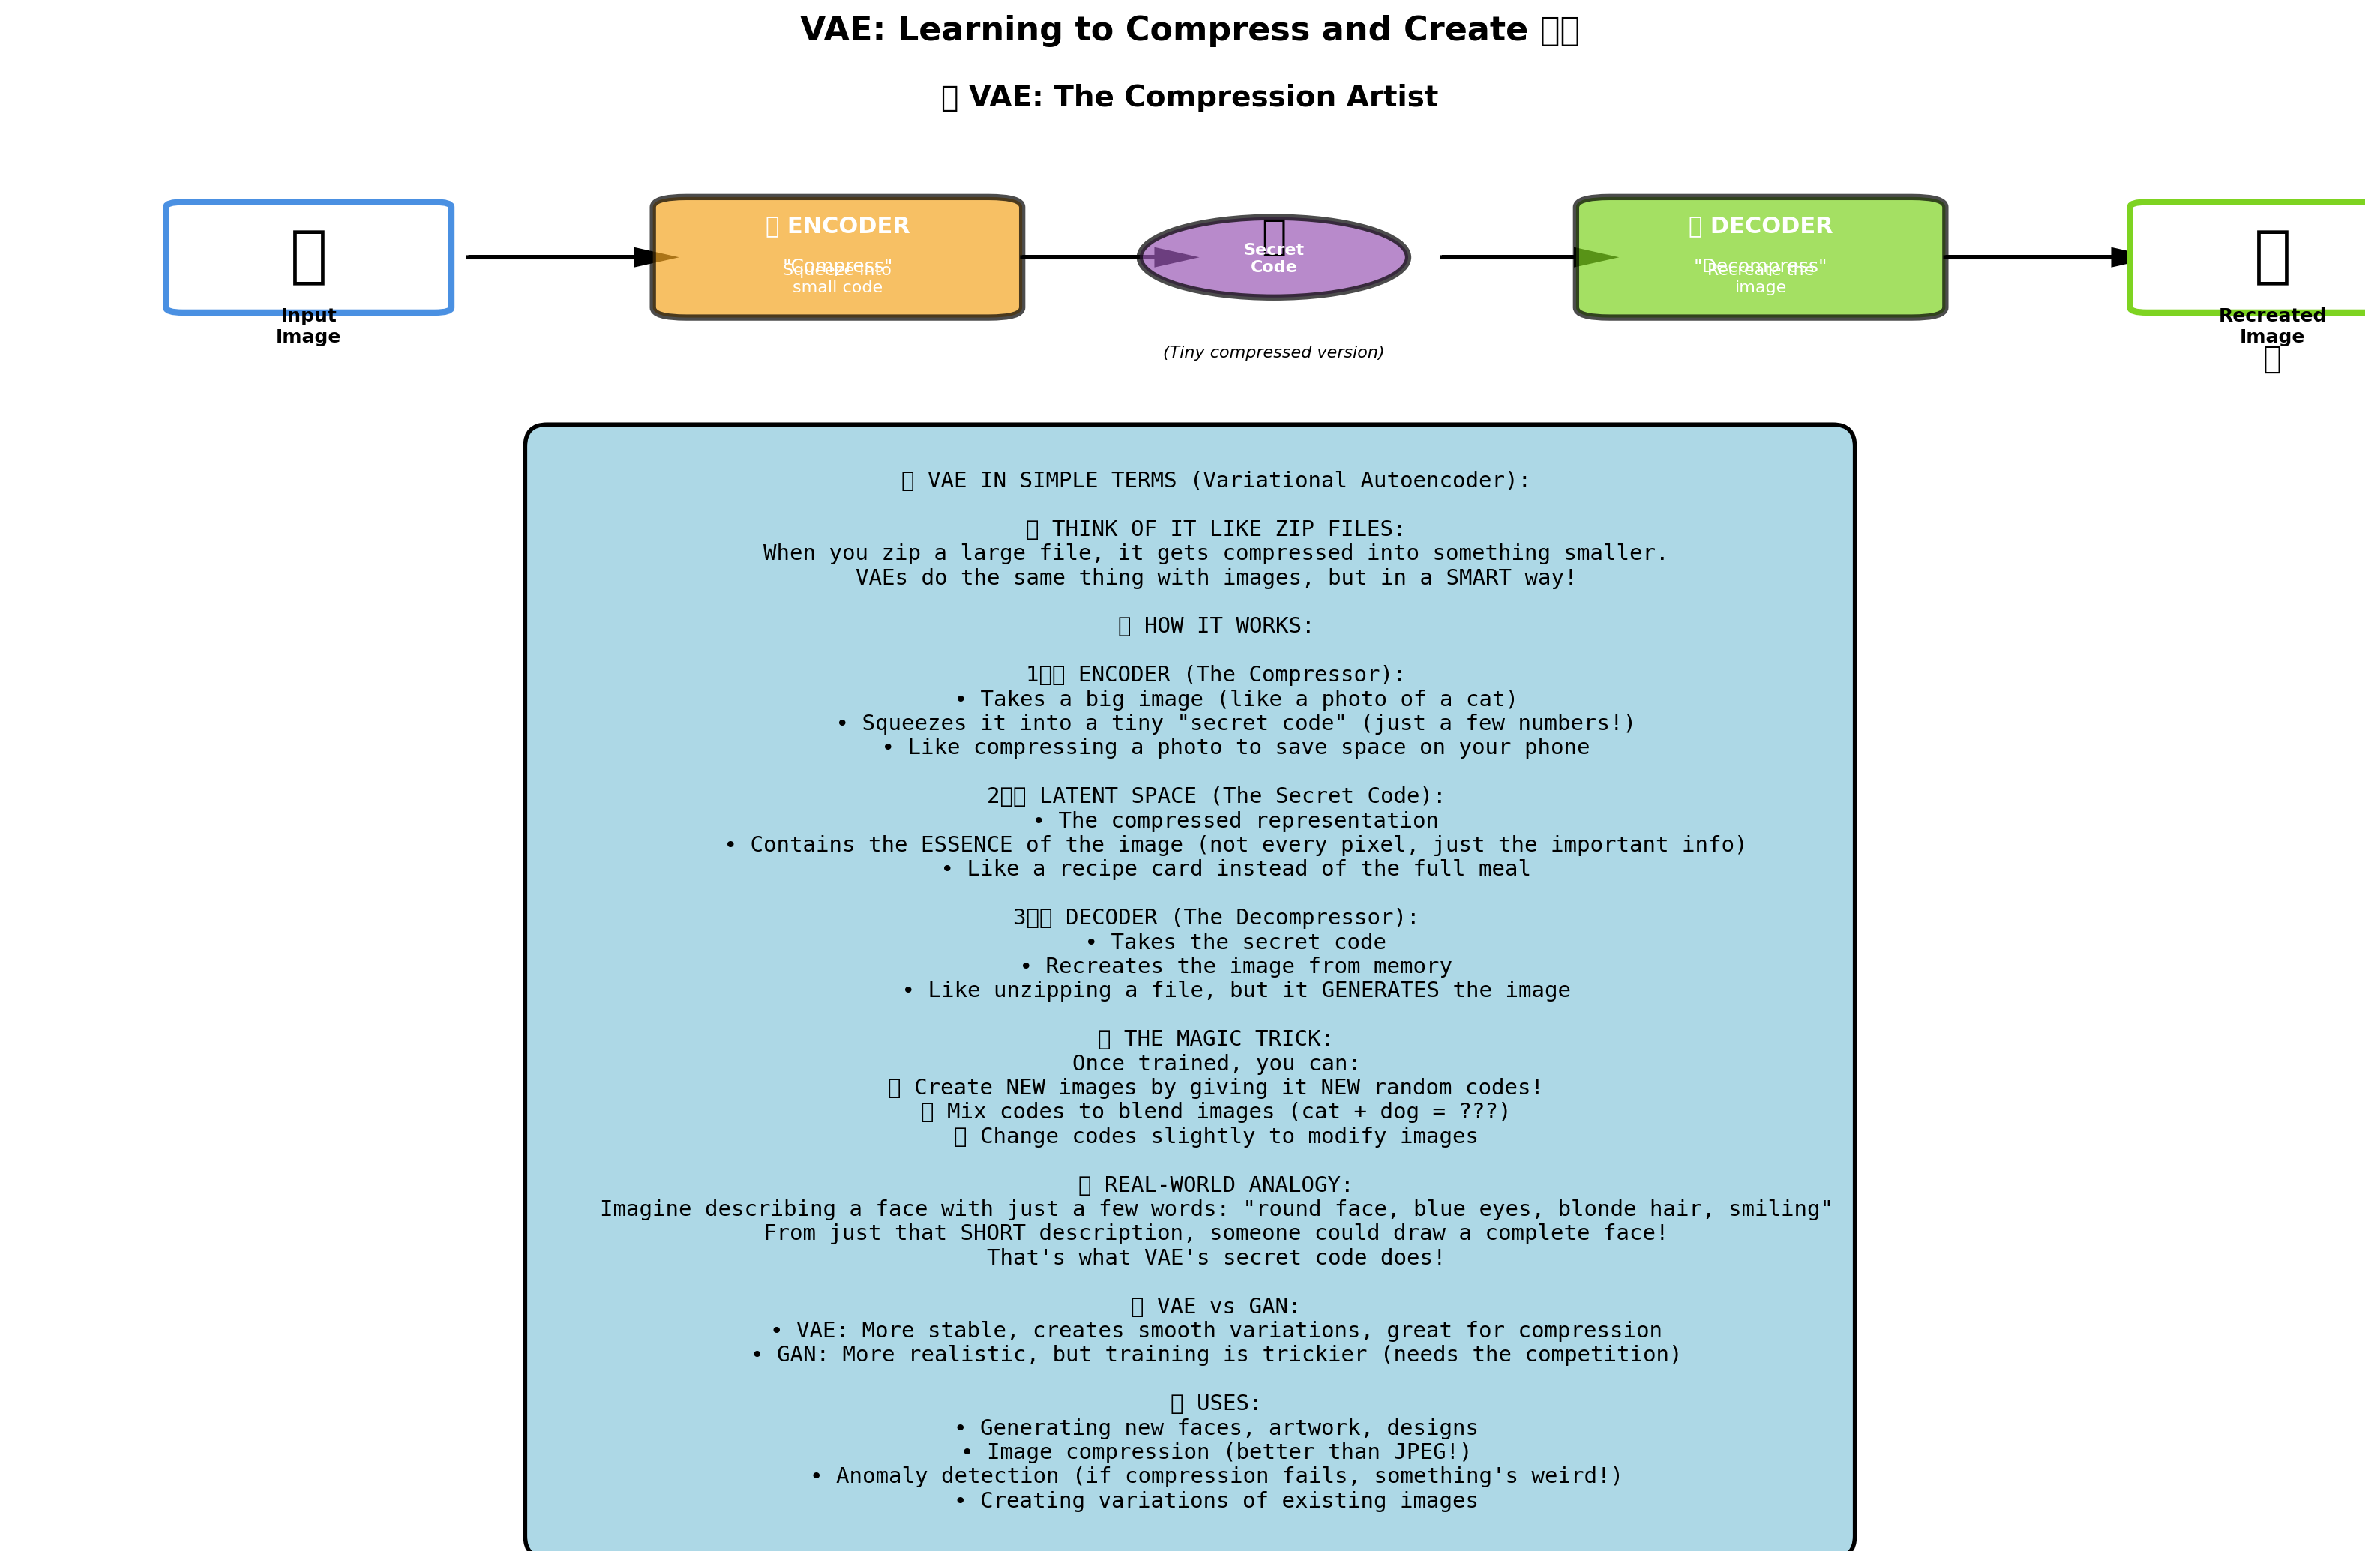
\includegraphics[width=0.85\textwidth]{../figures/vae_simple_concept.png}

\vspace{0.2cm}

\begin{block}{Simple Explanation}
\textbf{VAEs compress data into a small code, then decompress it:}
\begin{itemize}
\setlength{\itemsep}{3pt}
\item \textbf{Encoder:} Compress image into compact representation (like zip file)
\item \textbf{Latent Space:} The compressed "code" capturing key features
\item \textbf{Decoder:} Reconstruct image from the code
\item Can generate new images by sampling random codes!
\end{itemize}
\end{block}
\end{frame}

\begin{frame}{VAE Application: Anomaly Detection}
\begin{columns}[t]
\begin{column}{0.48\textwidth}
\begin{block}{Manufacturing Quality Control}
\textbf{How It Works:}
\begin{itemize}
\setlength{\itemsep}{2pt}
\item Train VAE on normal products
\item VAE learns what "normal" looks like
\item Defects reconstruct poorly
\item High reconstruction error = defect!
\end{itemize}
\end{block}

\vspace{0.15cm}

\begin{exampleblock}{Real Applications}
\begin{itemize}
\setlength{\itemsep}{2pt}
\item Detect scratches on surfaces
\item Find cracks in materials
\item Identify missing components
\item Automated quality inspection
\end{itemize}
\end{exampleblock}
\end{column}

\begin{column}{0.48\textwidth}
\begin{block}{Other Anomaly Detection Uses}
\begin{itemize}
\setlength{\itemsep}{2pt}
\item \textbf{Cybersecurity:} Detect network intrusions
\item \textbf{Finance:} Identify fraudulent transactions
\item \textbf{Healthcare:} Flag unusual patient vitals
\item \textbf{IoT:} Detect sensor failures
\end{itemize}
\end{block}

\vspace{0.15cm}

\begin{alertblock}{Advantage}
Works without labeled defect examples - learns from normal data only!
\end{alertblock}
\end{column}
\end{columns}
\end{frame}

\begin{frame}{VAE Application: Image Compression}
\begin{columns}[t]
\begin{column}{0.48\textwidth}
\begin{block}{Why VAEs for Compression?}
\textbf{Advantages over JPEG:}
\begin{itemize}
\setlength{\itemsep}{2pt}
\item Better quality at low bitrates
\item Learned compression (adapts to content)
\item Can compress to tiny sizes
\item Semantic preservation
\end{itemize}
\end{block}

\vspace{0.15cm}

\begin{exampleblock}{How It Works}
\begin{itemize}
\setlength{\itemsep}{2pt}
\item Encoder compresses to latent code
\item Store only the small code
\item Decoder reconstructs when needed
\item 10-100x smaller than JPEG
\end{itemize}
\end{exampleblock}
\end{column}

\begin{column}{0.48\textwidth}
\begin{block}{Real-World Uses}
\begin{itemize}
\setlength{\itemsep}{2pt}
\item Store medical imaging archives
\item Stream video at lower bandwidth
\item Compress satellite imagery
\item Mobile app image caching
\end{itemize}
\end{block}

\vspace{0.15cm}

\begin{alertblock}{Research Example}
Google's neural image compression beats JPEG by 50\% in quality metrics!
\end{alertblock}
\end{column}
\end{columns}
\end{frame}

\begin{frame}{VAE Application: Drug Molecule Generation}
\begin{columns}[t]
\begin{column}{0.48\textwidth}
\begin{block}{Pharmaceutical Discovery}
\textbf{Traditional Approach:}
\begin{itemize}
\setlength{\itemsep}{2pt}
\item Test millions of molecules
\item Takes 10+ years per drug
\item Costs billions of dollars
\item High failure rate
\end{itemize}
\end{block}

\vspace{0.15cm}

\begin{exampleblock}{VAE Approach}
\begin{itemize}
\setlength{\itemsep}{2pt}
\item Learn from existing drugs
\item Generate similar molecules
\item Optimize for target properties
\item Find candidates much faster
\end{itemize}
\end{exampleblock}
\end{column}

\begin{column}{0.48\textwidth}
\begin{block}{Real Pharmaceutical AI}
\begin{itemize}
\setlength{\itemsep}{2pt}
\item \textbf{Insilico Medicine:} Generated novel molecules
\item \textbf{Atomwise:} AI drug discovery platform
\item \textbf{BenevolentAI:} COVID-19 drug repurposing
\item Reduce discovery time by 75\%
\end{itemize}
\end{block}

\vspace{0.15cm}

\begin{alertblock}{Major Milestone}
First AI-discovered drug entered human trials in 2020!
\end{alertblock}
\end{column}
\end{columns}
\end{frame}

% ========================================
% Section: Transformers
% ========================================

\section{Transformers: The Revolution in AI}

\begin{frame}{Transformers: What Are They?}
\centering
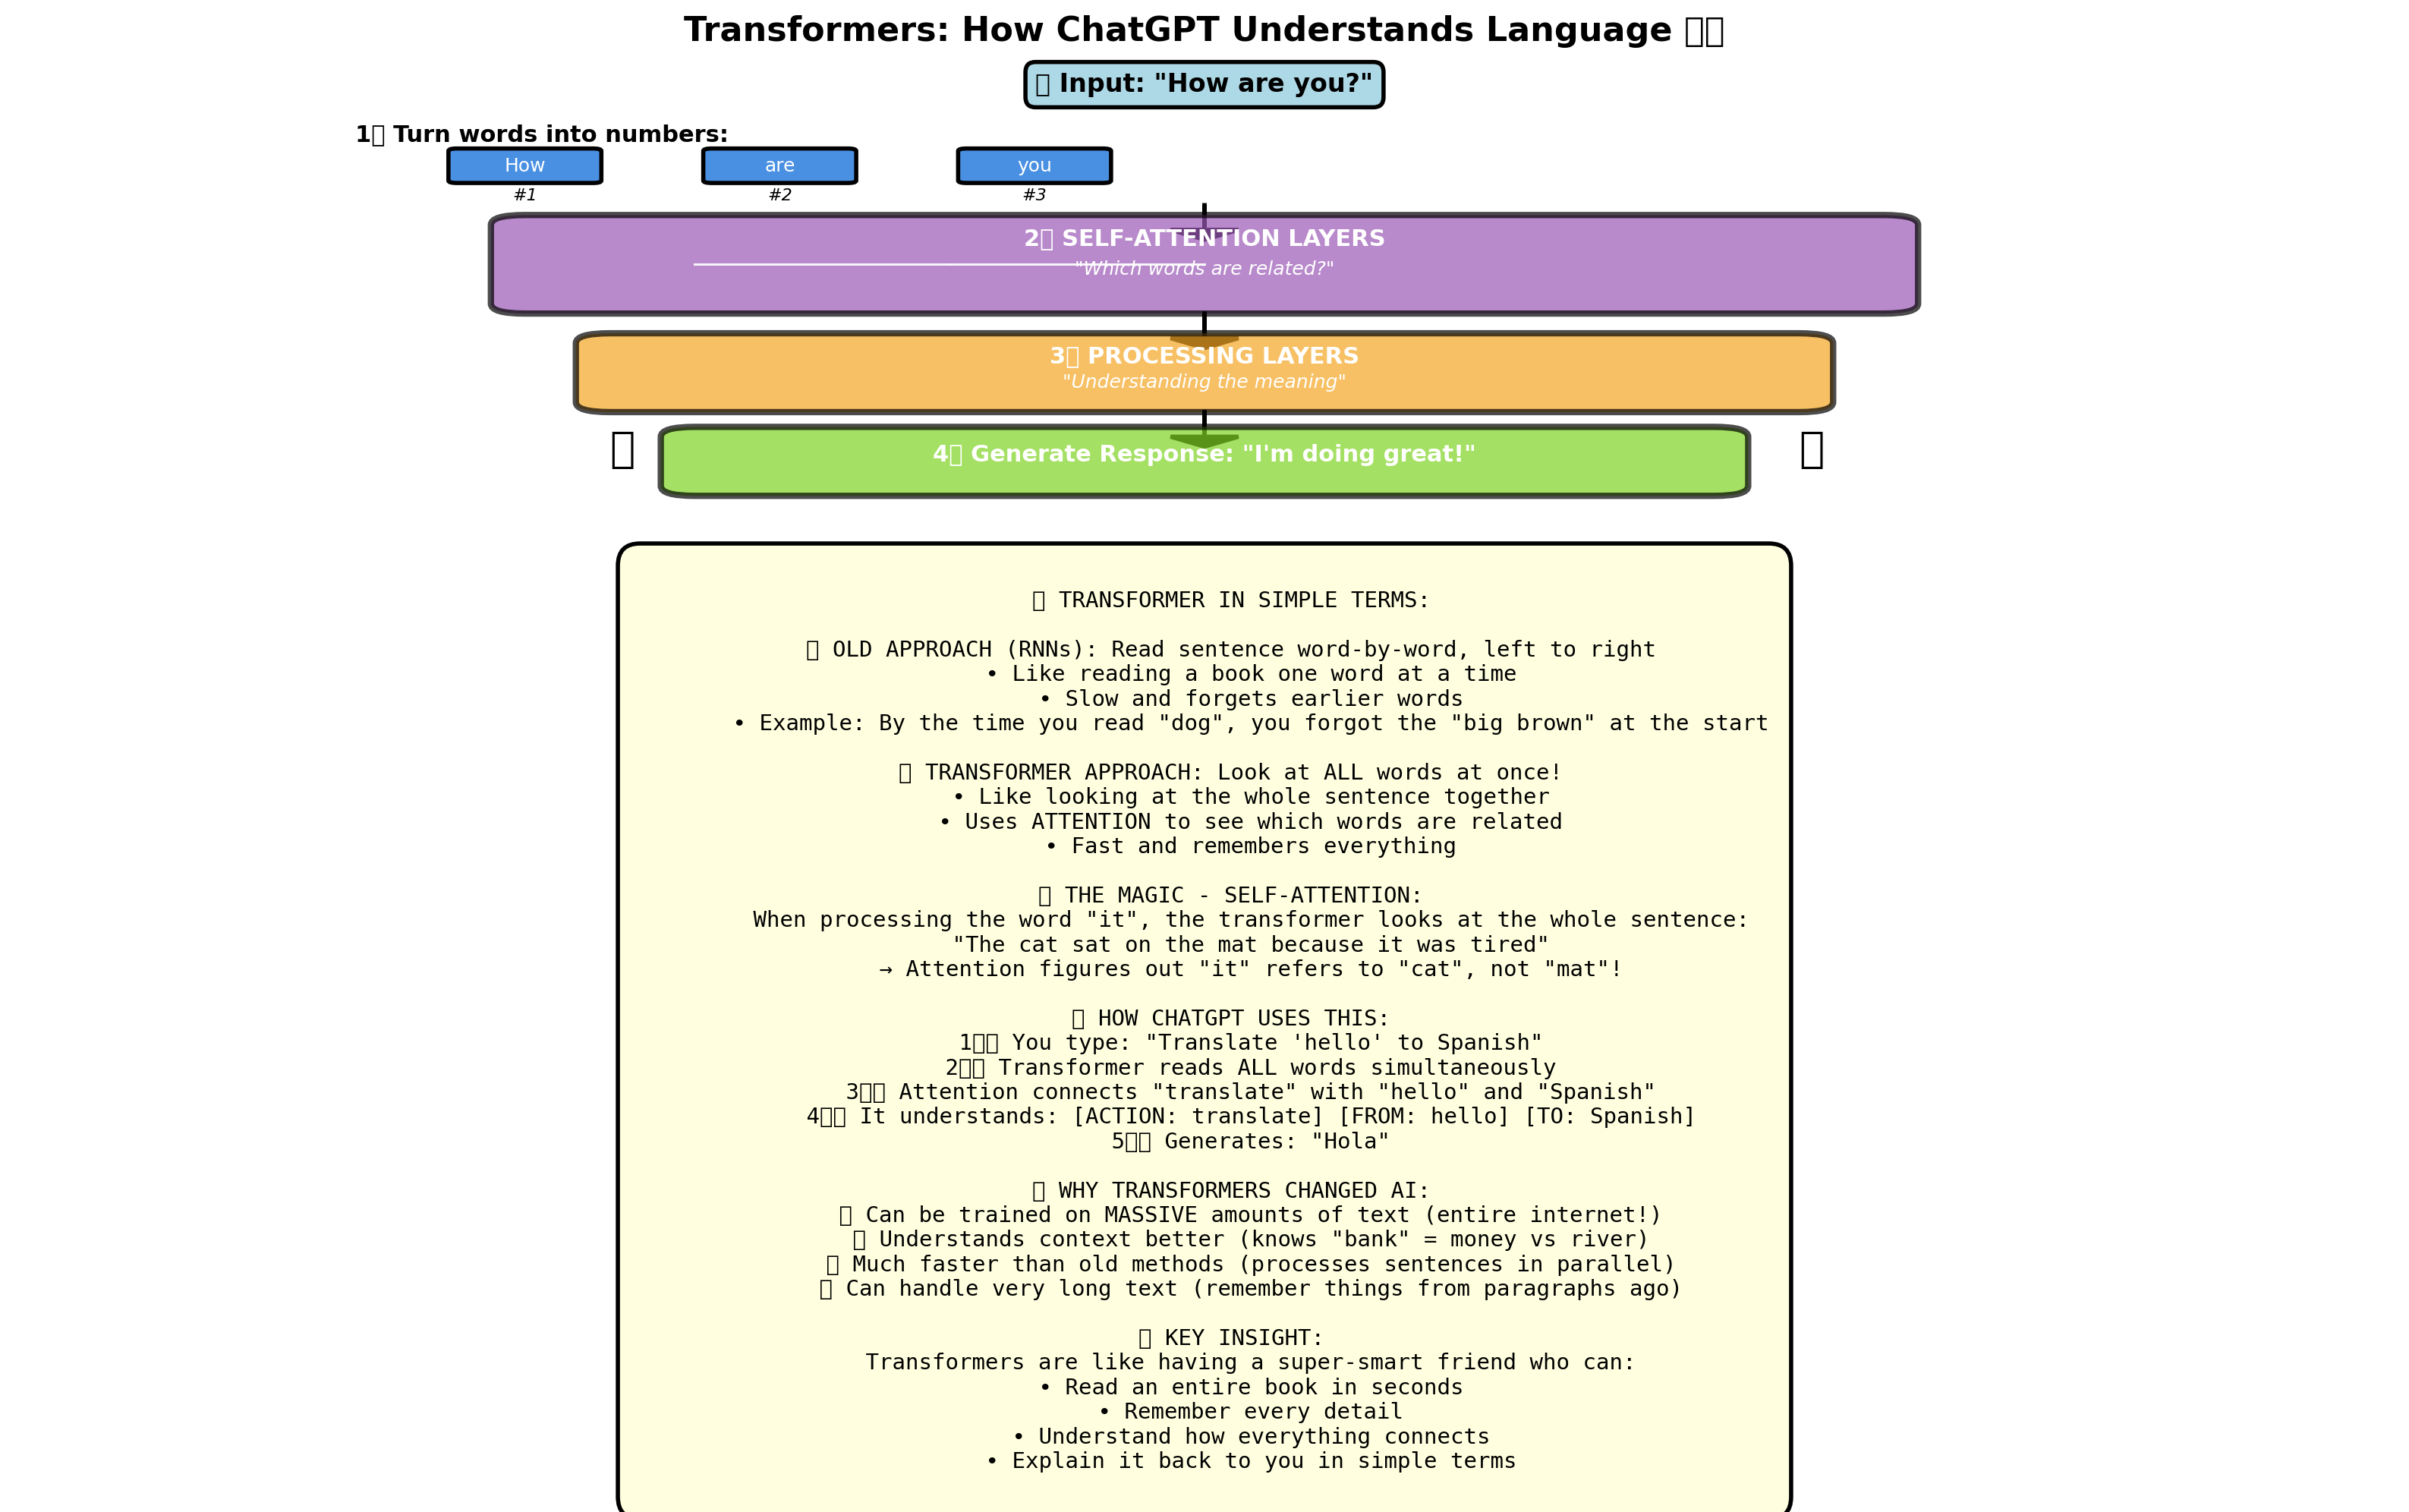
\includegraphics[width=0.85\textwidth]{../figures/transformer_simple_architecture.png}

\vspace{0.2cm}

\begin{block}{Simple Explanation}
\textbf{Transformers process sequences by paying attention to relevant parts:}
\begin{itemize}
\setlength{\itemsep}{3pt}
\item Designed for text, but work on images/audio too
\item Use "attention" to focus on important words
\item Process entire sequence at once (fast!)
\item Foundation of modern AI: GPT, BERT, ChatGPT
\end{itemize}
\end{block}
\end{frame}

\begin{frame}{Transformer Applications Overview}
\centering
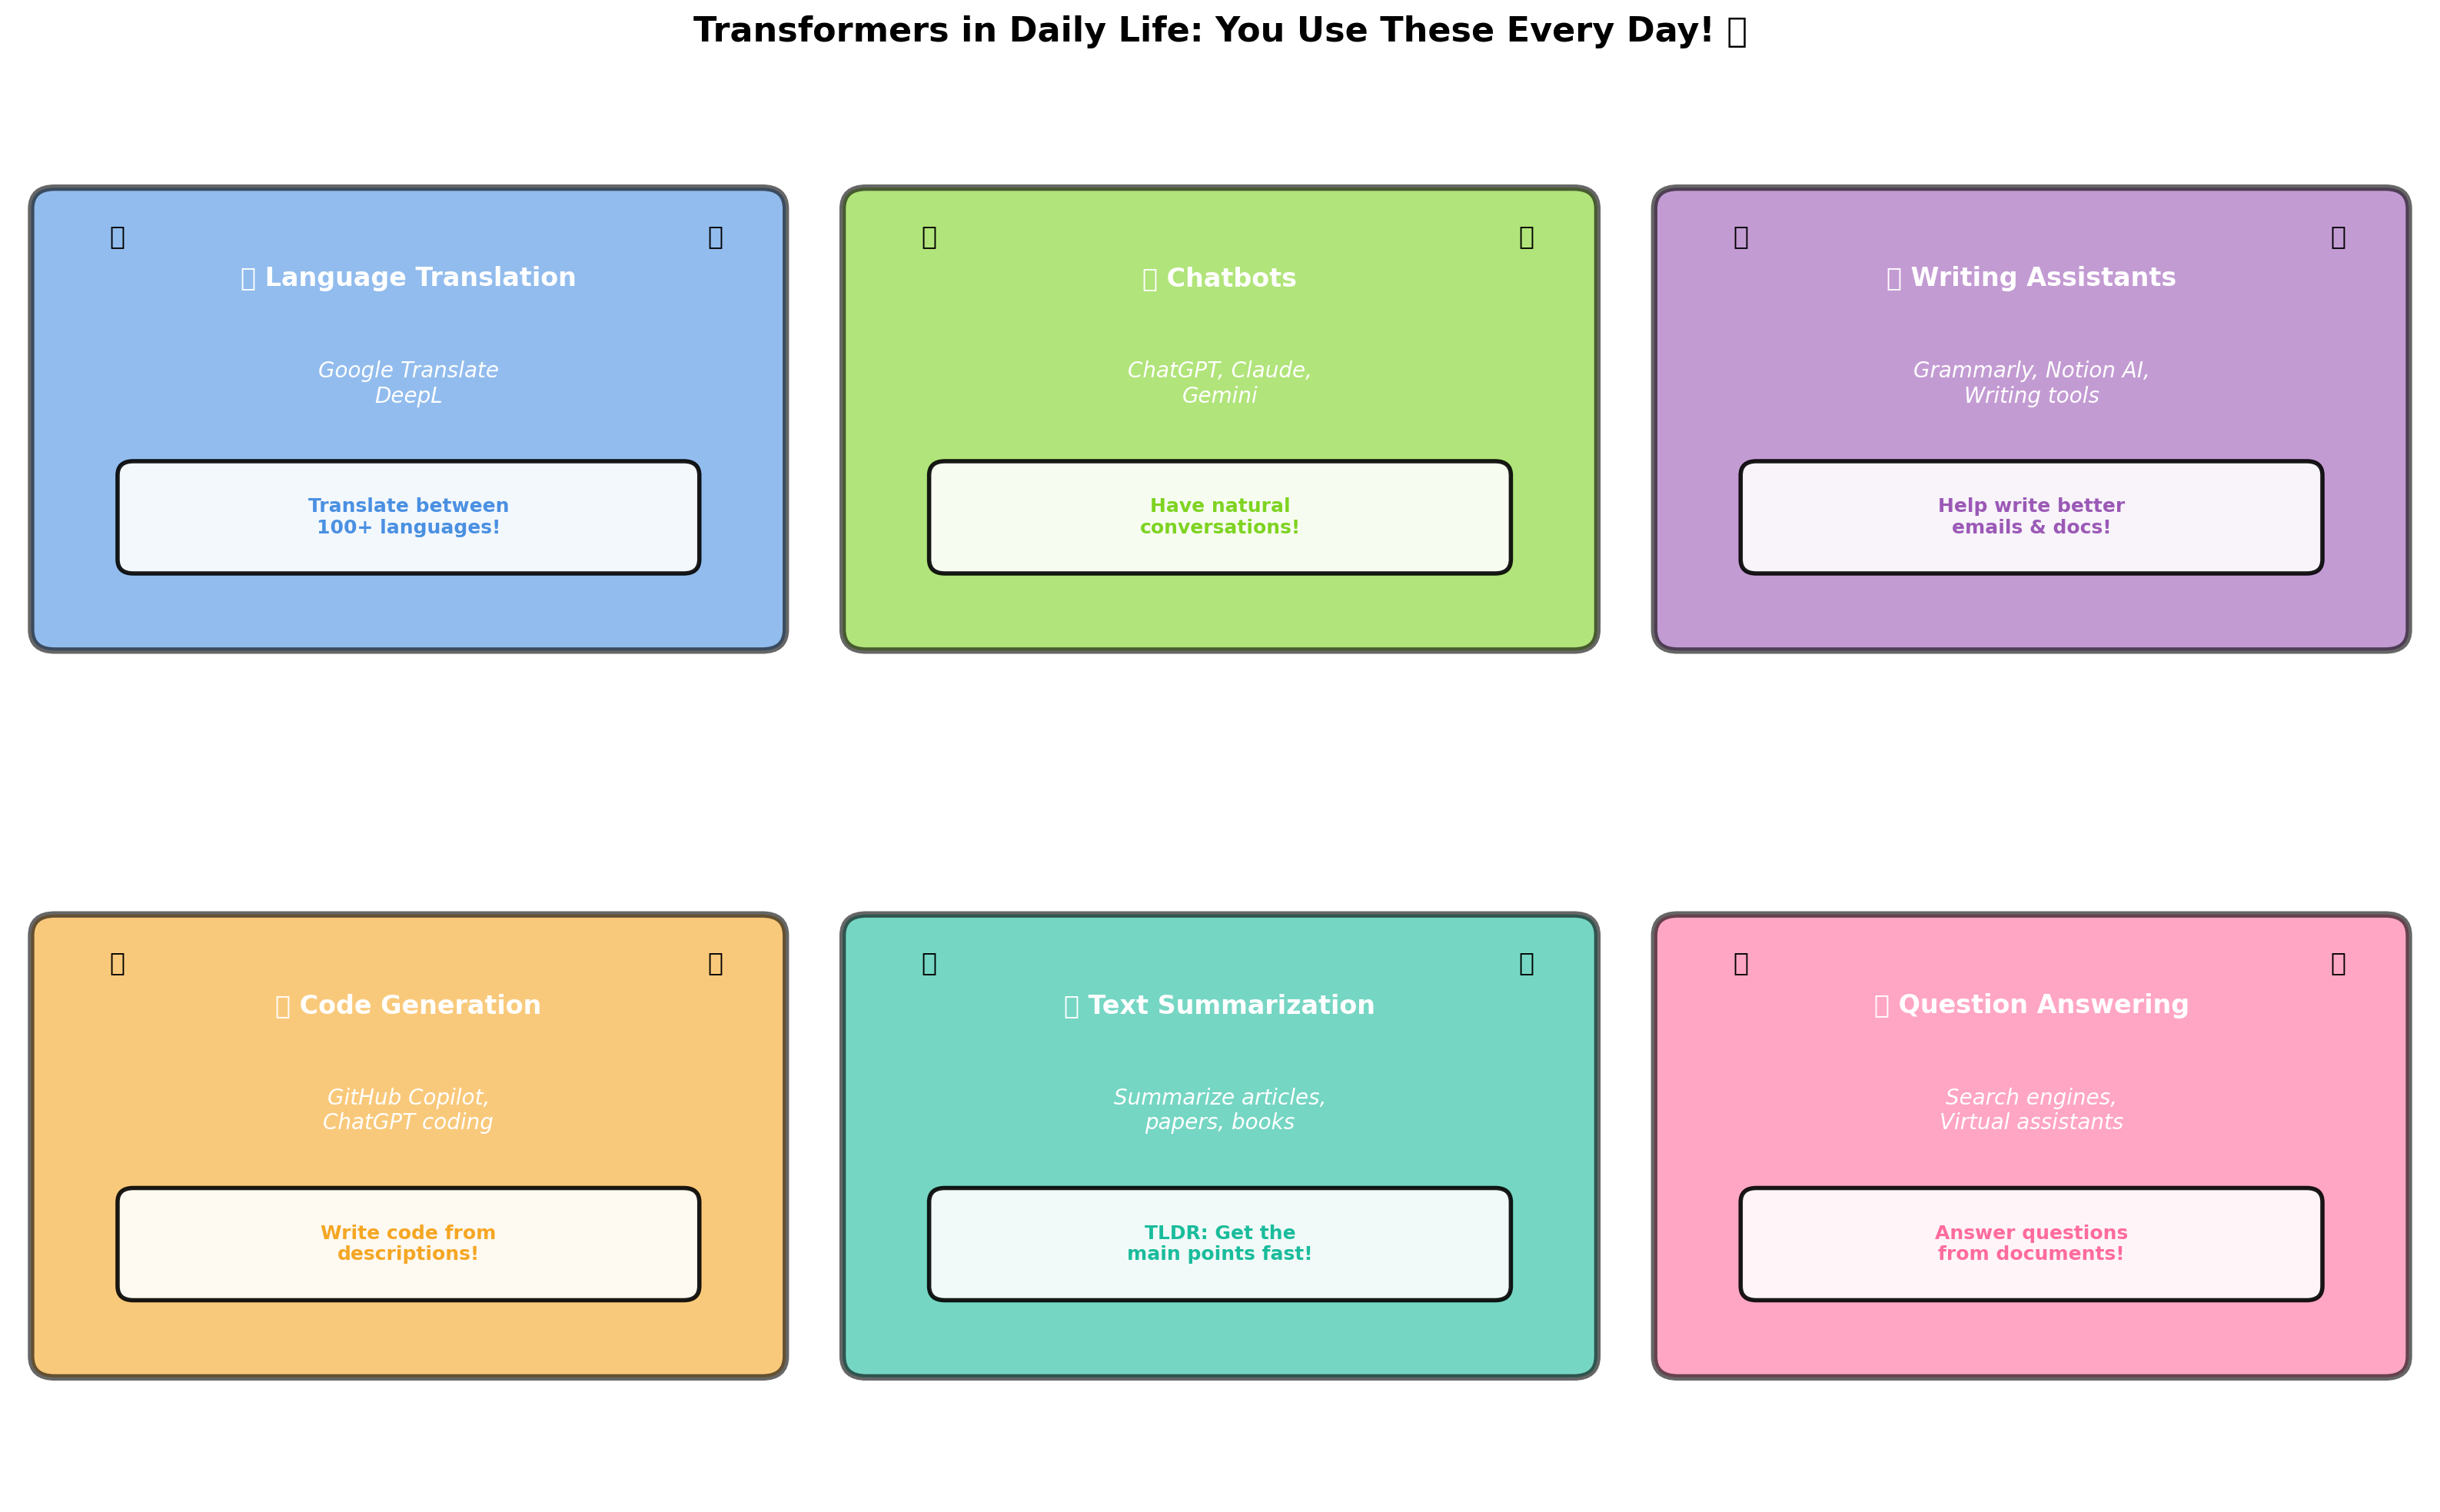
\includegraphics[width=0.88\textwidth]{../figures/transformer_applications.png}

\vspace{0.2cm}

\begin{alertblock}{Why Transformers Changed Everything}
Before 2017: RNNs struggled with long sequences. After 2017: Transformers enabled GPT, BERT, and the current AI revolution!
\end{alertblock}
\end{frame}

\begin{frame}{Transformer Application: ChatGPT}
\begin{columns}[t]
\begin{column}{0.48\textwidth}
\begin{block}{What ChatGPT Can Do}
\textbf{Capabilities:}
\begin{itemize}
\setlength{\itemsep}{2pt}
\item Answer questions
\item Write code and debug
\item Compose essays and emails
\item Explain complex topics
\item Translate languages
\item Creative writing
\end{itemize}
\end{block}

\vspace{0.15cm}

\begin{exampleblock}{Real Usage Statistics}
\begin{itemize}
\setlength{\itemsep}{2pt}
\item 100+ million weekly users
\item Fastest-growing consumer app
\item Used in 185+ countries
\end{itemize}
\end{exampleblock}
\end{column}

\begin{column}{0.48\textwidth}
\begin{block}{How Students Use It}
\begin{itemize}
\setlength{\itemsep}{2pt}
\item Homework help and tutoring
\item Research assistance
\item Programming debugging
\item Study guide creation
\item Language learning
\item Career advice
\end{itemize}
\end{block}

\vspace{0.15cm}

\begin{alertblock}{Built With Transformers}
GPT-4 uses a massive transformer with 175+ billion parameters!
\end{alertblock}
\end{column}
\end{columns}
\end{frame}

\begin{frame}{Transformer Application: Google Translate}
\begin{columns}[t]
\begin{column}{0.48\textwidth}
\begin{block}{Old vs New Approach}
\textbf{Before Transformers (2016):}
\begin{itemize}
\setlength{\itemsep}{2pt}
\item Phrase-based translation
\item Limited context understanding
\item Often awkward output
\end{itemize}

\vspace{0.1cm}

\textbf{After Transformers (2017+):}
\begin{itemize}
\setlength{\itemsep}{2pt}
\item Sentence-level context
\item Natural, fluent translations
\item 60\% reduction in errors
\end{itemize}
\end{block}
\end{column}

\begin{column}{0.48\textwidth}
\begin{exampleblock}{Features Powered by Transformers}
\begin{itemize}
\setlength{\itemsep}{2pt}
\item 133 languages supported
\item Real-time conversation mode
\item Camera translation (point and translate)
\item Offline translation
\item Context-aware results
\end{itemize}
\end{exampleblock}

\vspace{0.15cm}

\begin{alertblock}{Daily Impact}
500+ million people use Google Translate every day!
\end{alertblock}
\end{column}
\end{columns}
\end{frame}

\begin{frame}{Transformer Application: GitHub Copilot}
\begin{columns}[t]
\begin{column}{0.48\textwidth}
\begin{block}{AI Pair Programmer}
\textbf{What Copilot Does:}
\begin{itemize}
\setlength{\itemsep}{2pt}
\item Suggests code as you type
\item Writes entire functions
\item Explains existing code
\item Converts comments to code
\item Generates tests
\item Fixes bugs
\end{itemize}
\end{block}

\vspace{0.15cm}

\begin{exampleblock}{Real Developer Impact}
\begin{itemize}
\setlength{\itemsep}{2pt}
\item 46\% of code written by AI
\item 55\% faster task completion
\item Used by 1.2 million developers
\end{itemize}
\end{exampleblock}
\end{column}

\begin{column}{0.48\textwidth}
\begin{block}{How It Works}
\begin{itemize}
\setlength{\itemsep}{2pt}
\item Built on GPT (Codex model)
\item Trained on billions of lines of code
\item Understands context from your files
\item Suggests in real-time
\item Supports 12+ programming languages
\end{itemize}
\end{block}

\vspace{0.15cm}

\begin{alertblock}{For Students}
Great learning tool - see how experts solve problems!
\end{alertblock}
\end{column}
\end{columns}
\end{frame}

\begin{frame}{Transformer Application: Email Auto-Complete}
\begin{columns}[t]
\begin{column}{0.48\textwidth}
\begin{block}{Gmail Smart Compose}
\textbf{Features:}
\begin{itemize}
\setlength{\itemsep}{2pt}
\item Suggests next words/sentences
\item Learns your writing style
\item Adapts to context
\item Multi-language support
\item Works on mobile too
\end{itemize}
\end{block}

\vspace{0.15cm}

\begin{exampleblock}{Time Savings}
\begin{itemize}
\setlength{\itemsep}{2pt}
\item Average user saves 1 billion characters/week
\item Reduces writing time by 11\%
\item 4+ billion emails use it daily
\end{itemize}
\end{exampleblock}
\end{column}

\begin{column}{0.48\textwidth}
\begin{block}{Other Email AI Features}
\begin{itemize}
\setlength{\itemsep}{2pt}
\item \textbf{Smart Reply:} Suggest full responses
\item \textbf{Subject suggestions:} Auto-generate subjects
\item \textbf{Tone adjustment:} Make emails more formal
\item \textbf{Grammar correction:} Fix mistakes
\end{itemize}
\end{block}

\vspace{0.15cm}

\begin{alertblock}{All Powered by Transformers}
These "small" conveniences use the same tech as ChatGPT!
\end{alertblock}
\end{column}
\end{columns}
\end{frame}

\begin{frame}{Transformer Application: Document Summarization}
\begin{columns}[t]
\begin{column}{0.48\textwidth}
\begin{block}{Automatic Summarization}
\textbf{What It Does:}
\begin{itemize}
\setlength{\itemsep}{2pt}
\item Read long documents
\item Extract key points
\item Generate concise summary
\item Preserve important details
\item Save reading time
\end{itemize}
\end{block}

\vspace{0.15cm}

\begin{exampleblock}{Real Products}
\begin{itemize}
\setlength{\itemsep}{2pt}
\item \textbf{Microsoft Word:} Auto-summarize
\item \textbf{Slack:} Thread summaries
\item \textbf{Notion AI:} Note summarization
\item \textbf{Chrome extensions:} Web page summaries
\end{itemize}
\end{exampleblock}
\end{column}

\begin{column}{0.48\textwidth}
\begin{block}{Use Cases}
\begin{itemize}
\setlength{\itemsep}{2pt}
\item Research paper summaries
\item News article digests
\item Legal document review
\item Meeting notes condensation
\item Customer feedback analysis
\end{itemize}
\end{block}

\vspace{0.15cm}

\begin{alertblock}{Productivity Boost}
Lawyers using AI summarization save 60\% of document review time!
\end{alertblock}
\end{column}
\end{columns}
\end{frame}

\begin{frame}{Vision Transformers: Images Meet Transformers}
\centering
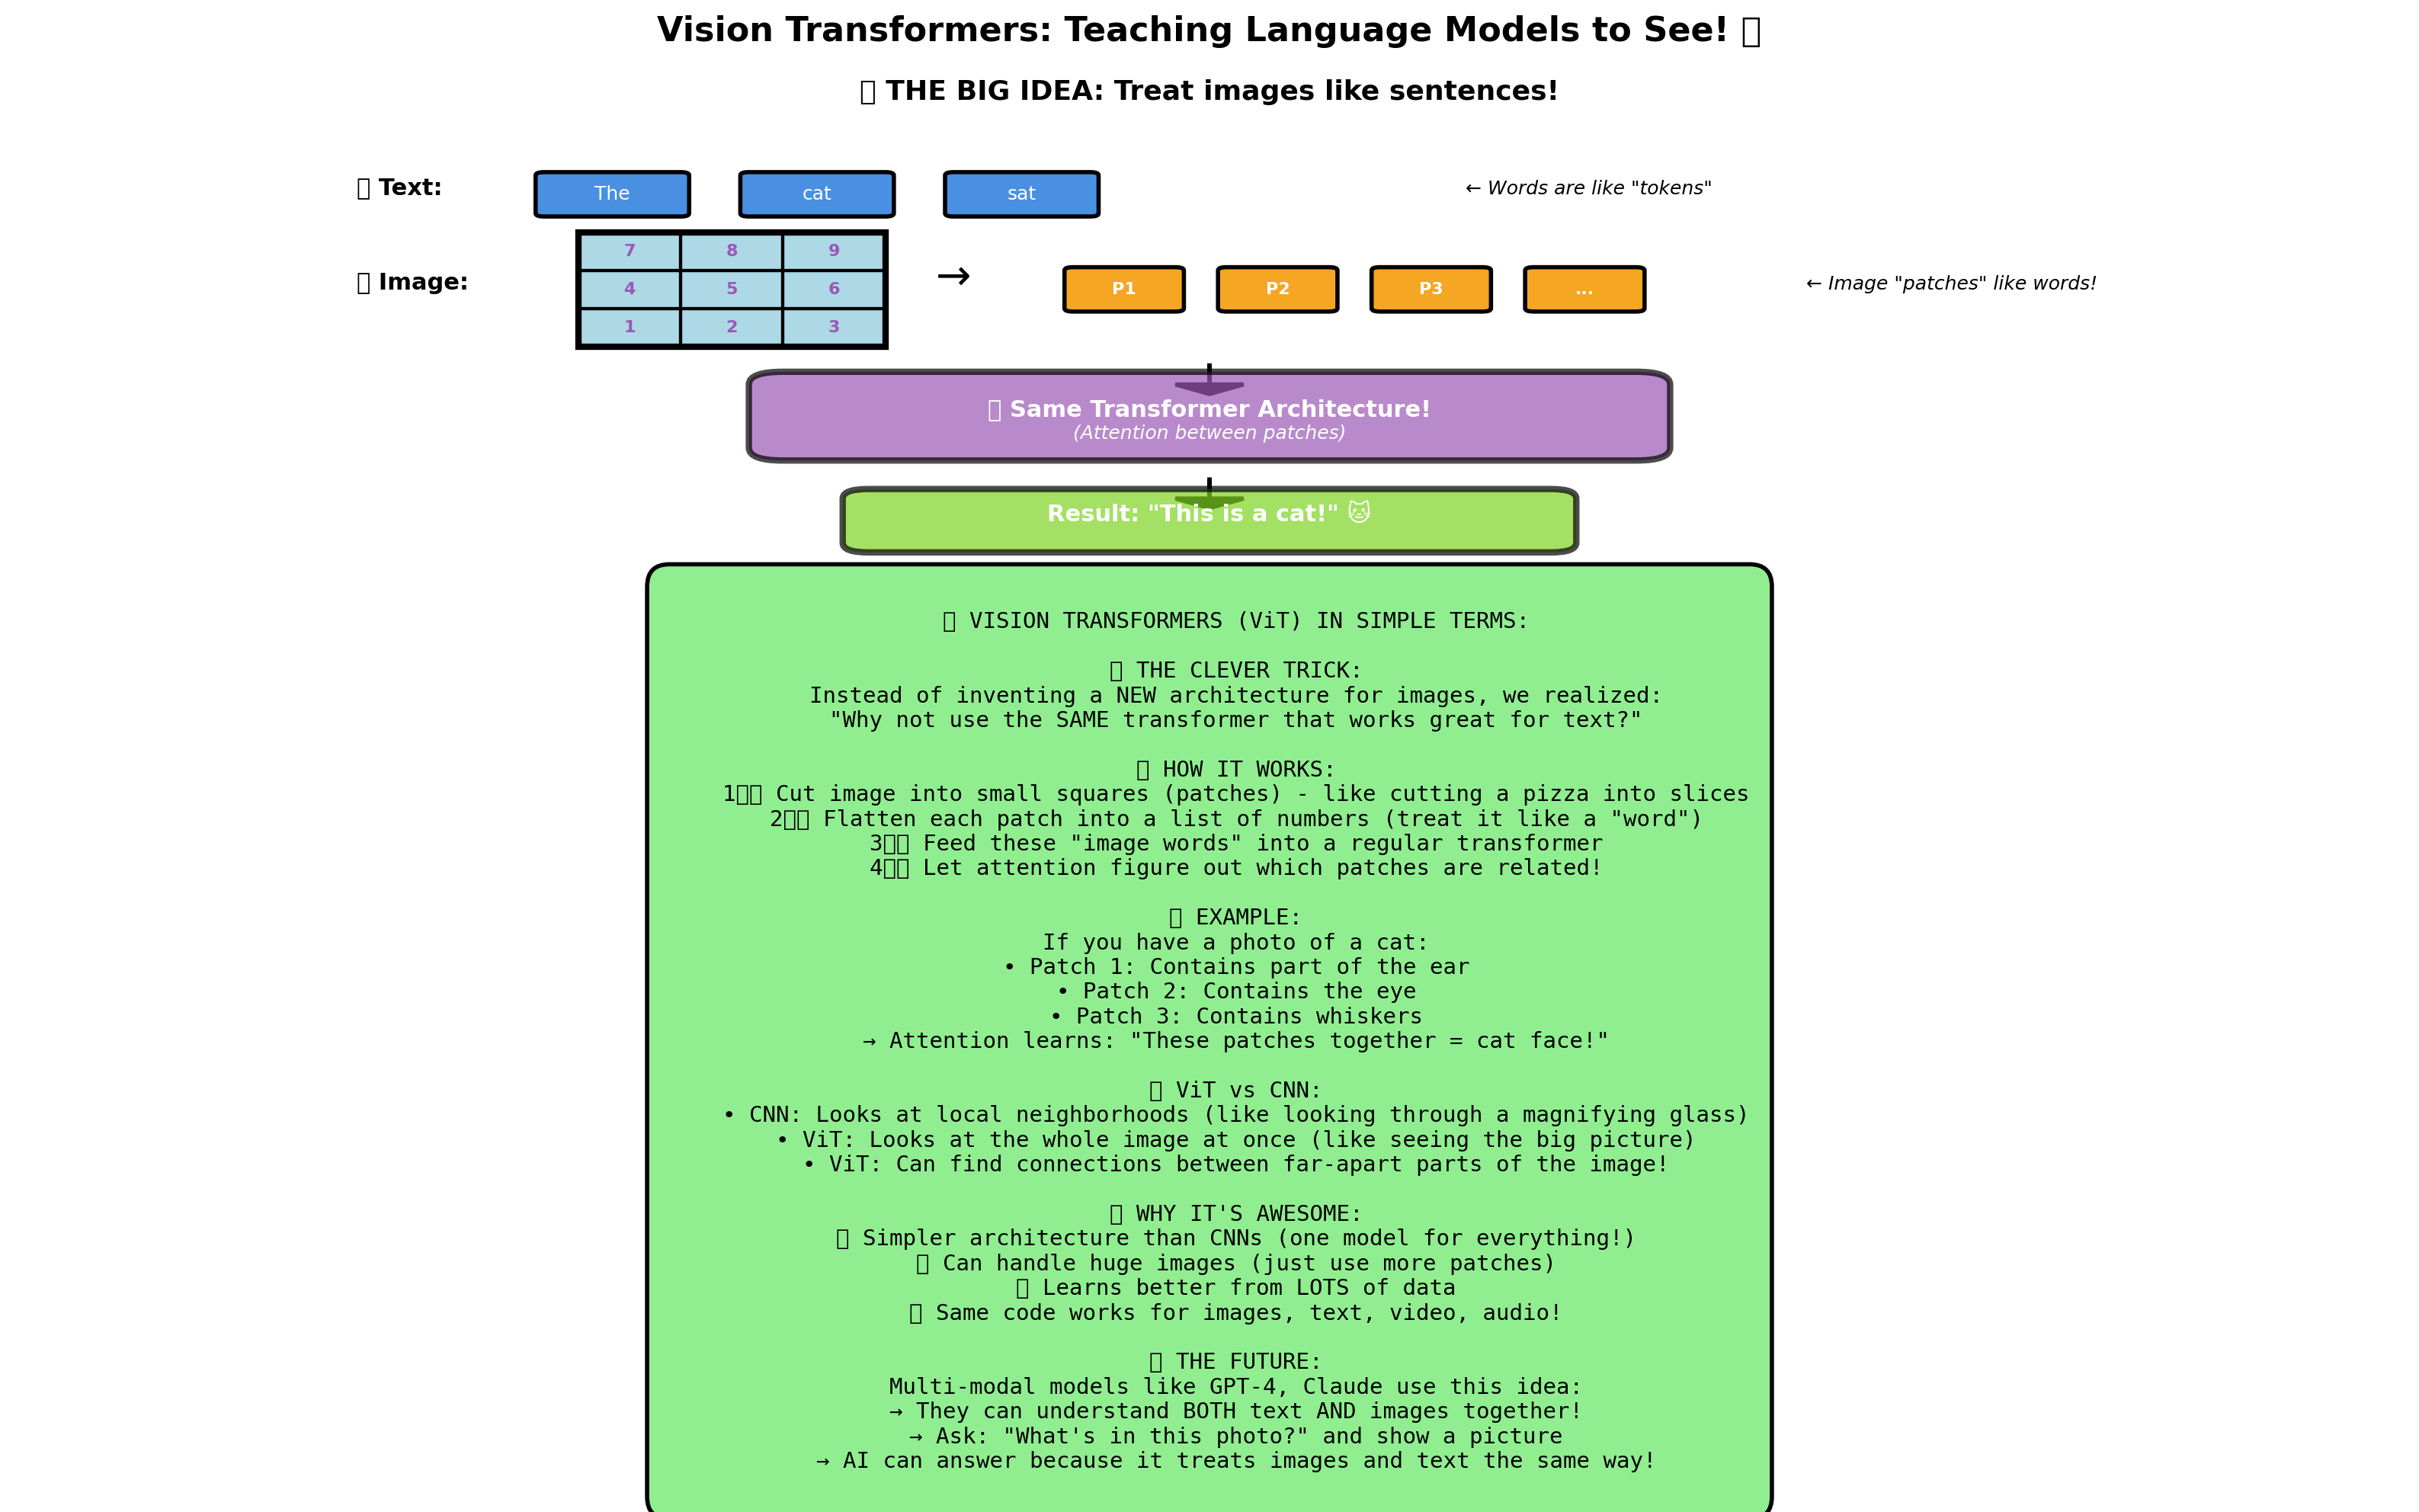
\includegraphics[width=0.85\textwidth]{../figures/vision_transformer_concept.png}

\vspace{0.2cm}

\begin{block}{Vision Transformers (ViT)}
\textbf{Applying transformers to images:}
\begin{itemize}
\setlength{\itemsep}{2pt}
\item Break image into patches (like words)
\item Apply transformer attention to patches
\item Often better than CNNs with enough data
\item Used in DALL-E, Imagen, latest AI systems
\end{itemize}
\end{block}
\end{frame}

% ========================================
% Section: Diffusion Models
% ========================================

\section{Diffusion Models: The Newest Revolution}

\begin{frame}{Diffusion Models: How They Work}
\centering
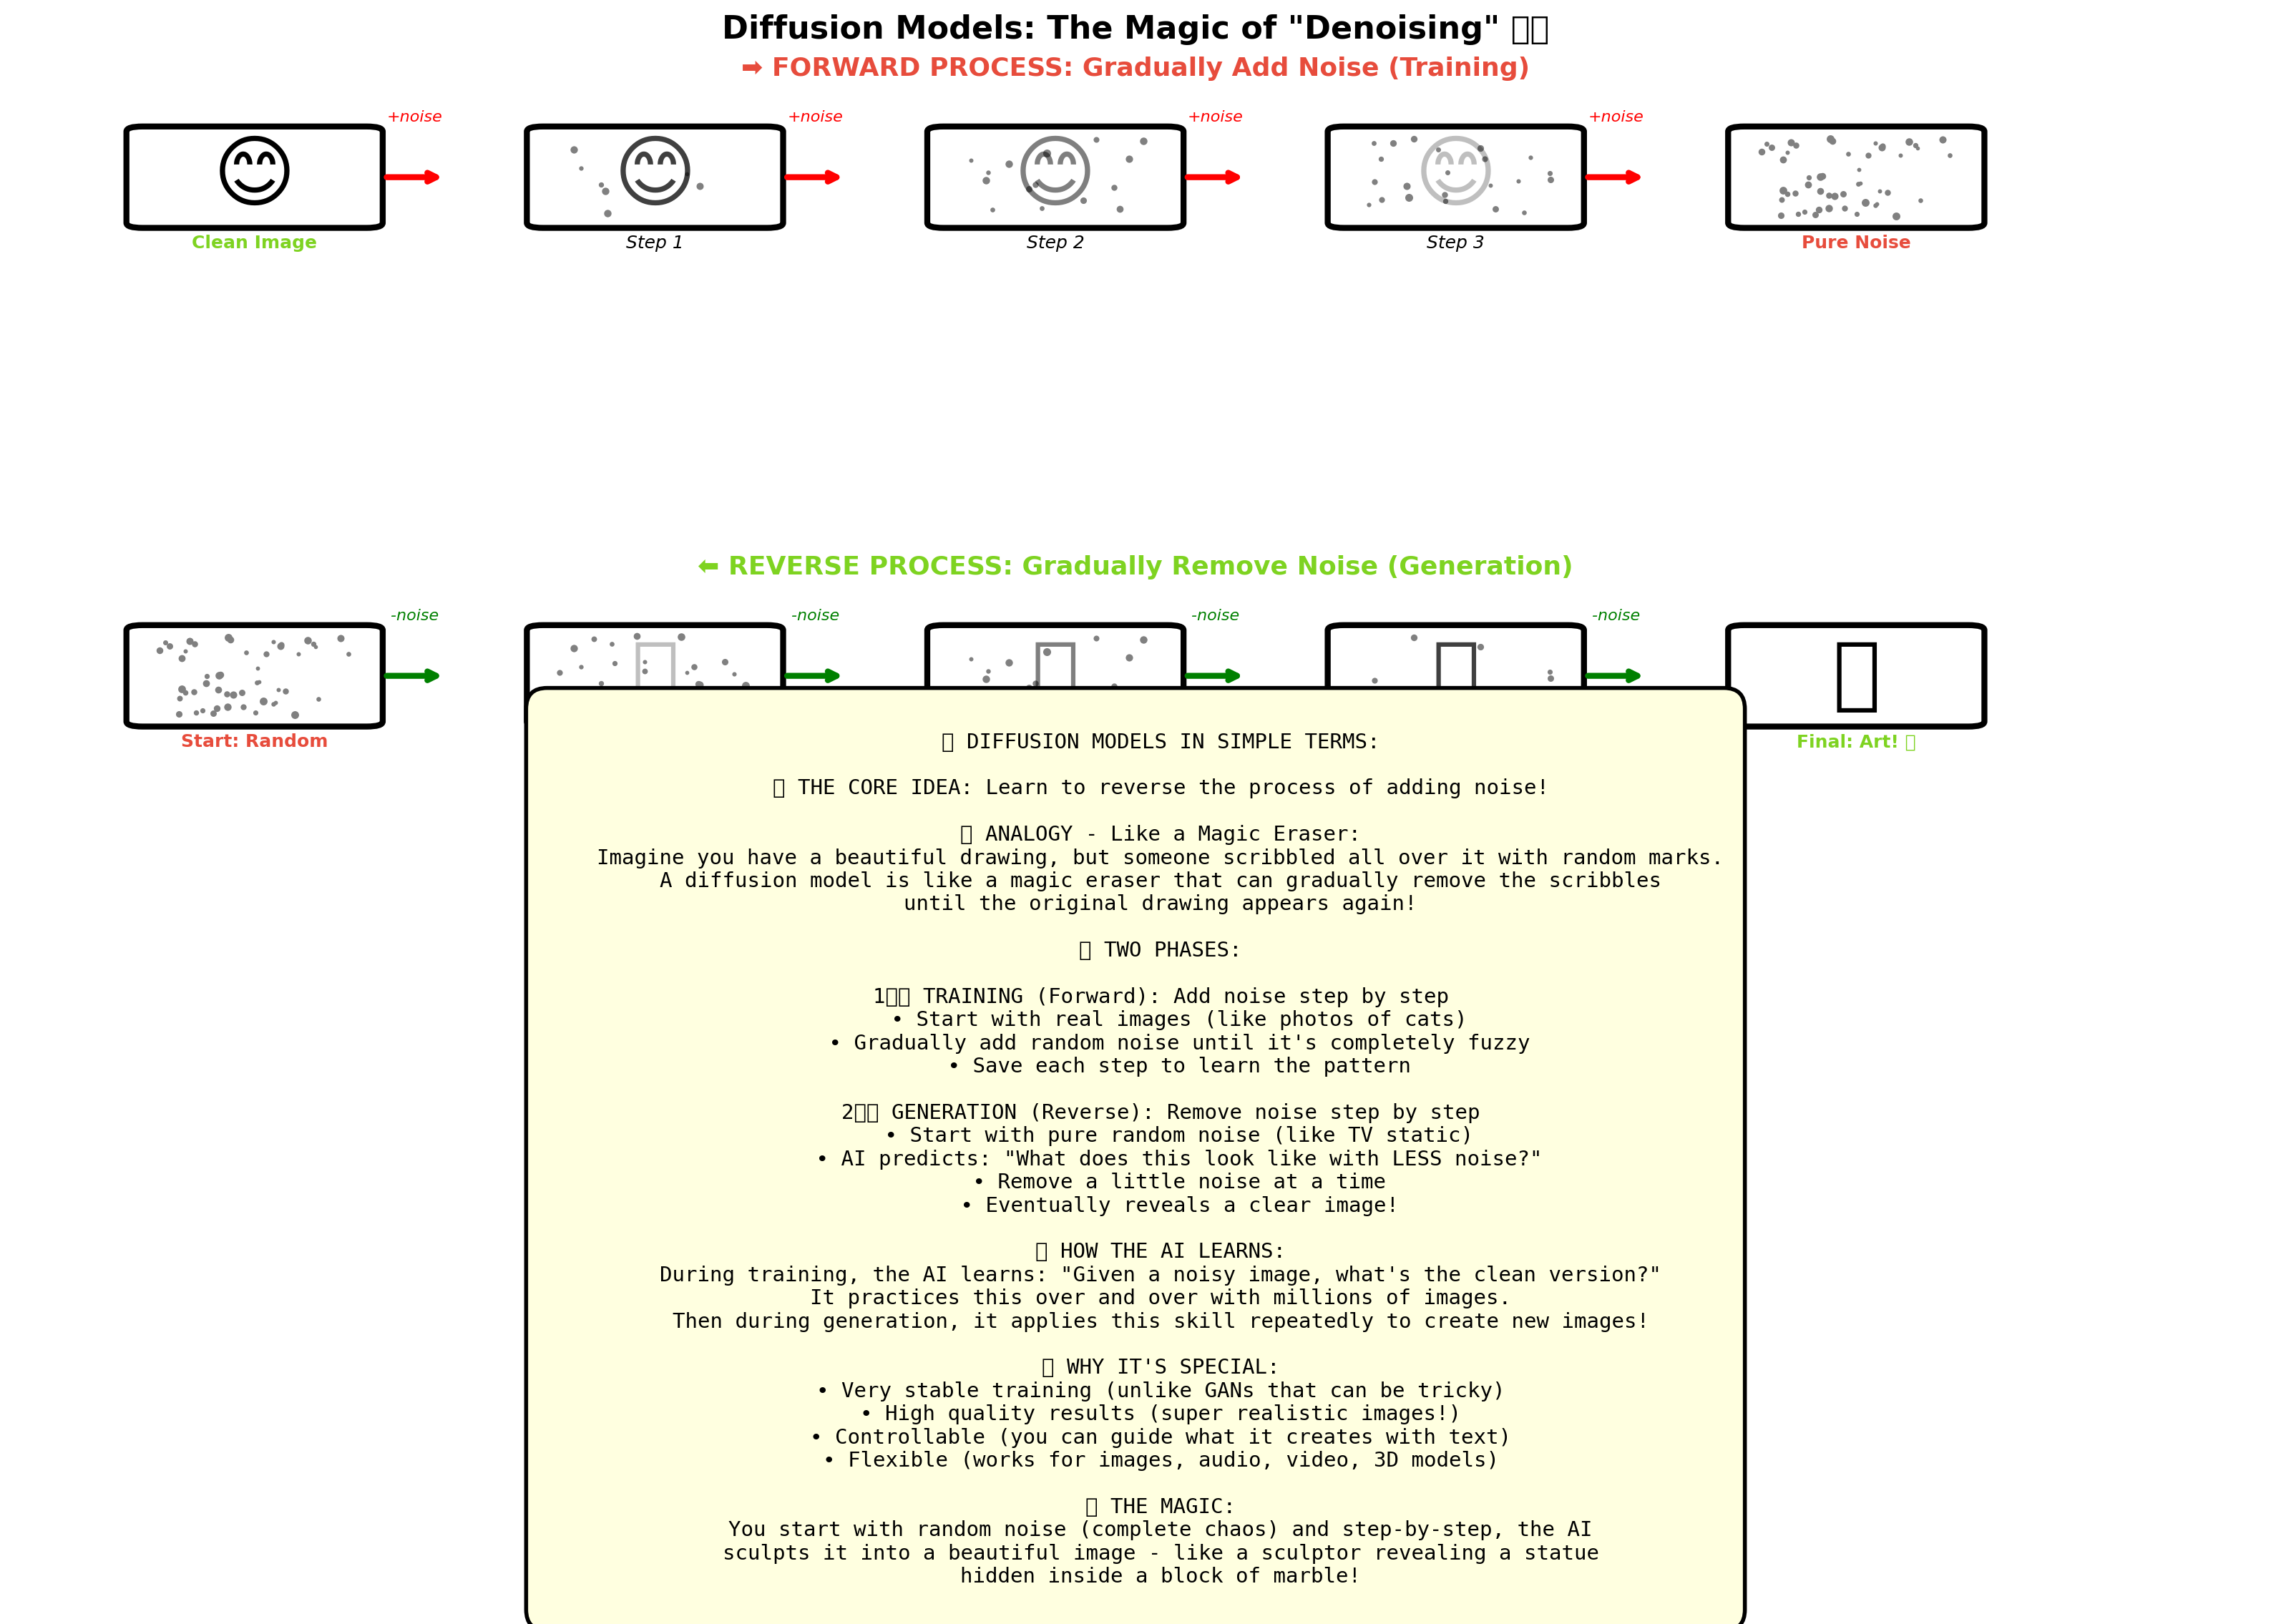
\includegraphics[width=0.88\textwidth]{../figures/diffusion_simple_concept.png}

\vspace{0.2cm}

\begin{block}{Simple Explanation}
\textbf{Create images by gradually removing noise:}
\begin{itemize}
\setlength{\itemsep}{3pt}
\item Start with pure random noise
\item Gradually remove noise step-by-step
\item Guided by text description
\item End with high-quality image
\item Like a sculptor revealing a statue from marble!
\end{itemize}
\end{block}
\end{frame}

\begin{frame}{Diffusion vs GANs vs VAEs}
\centering
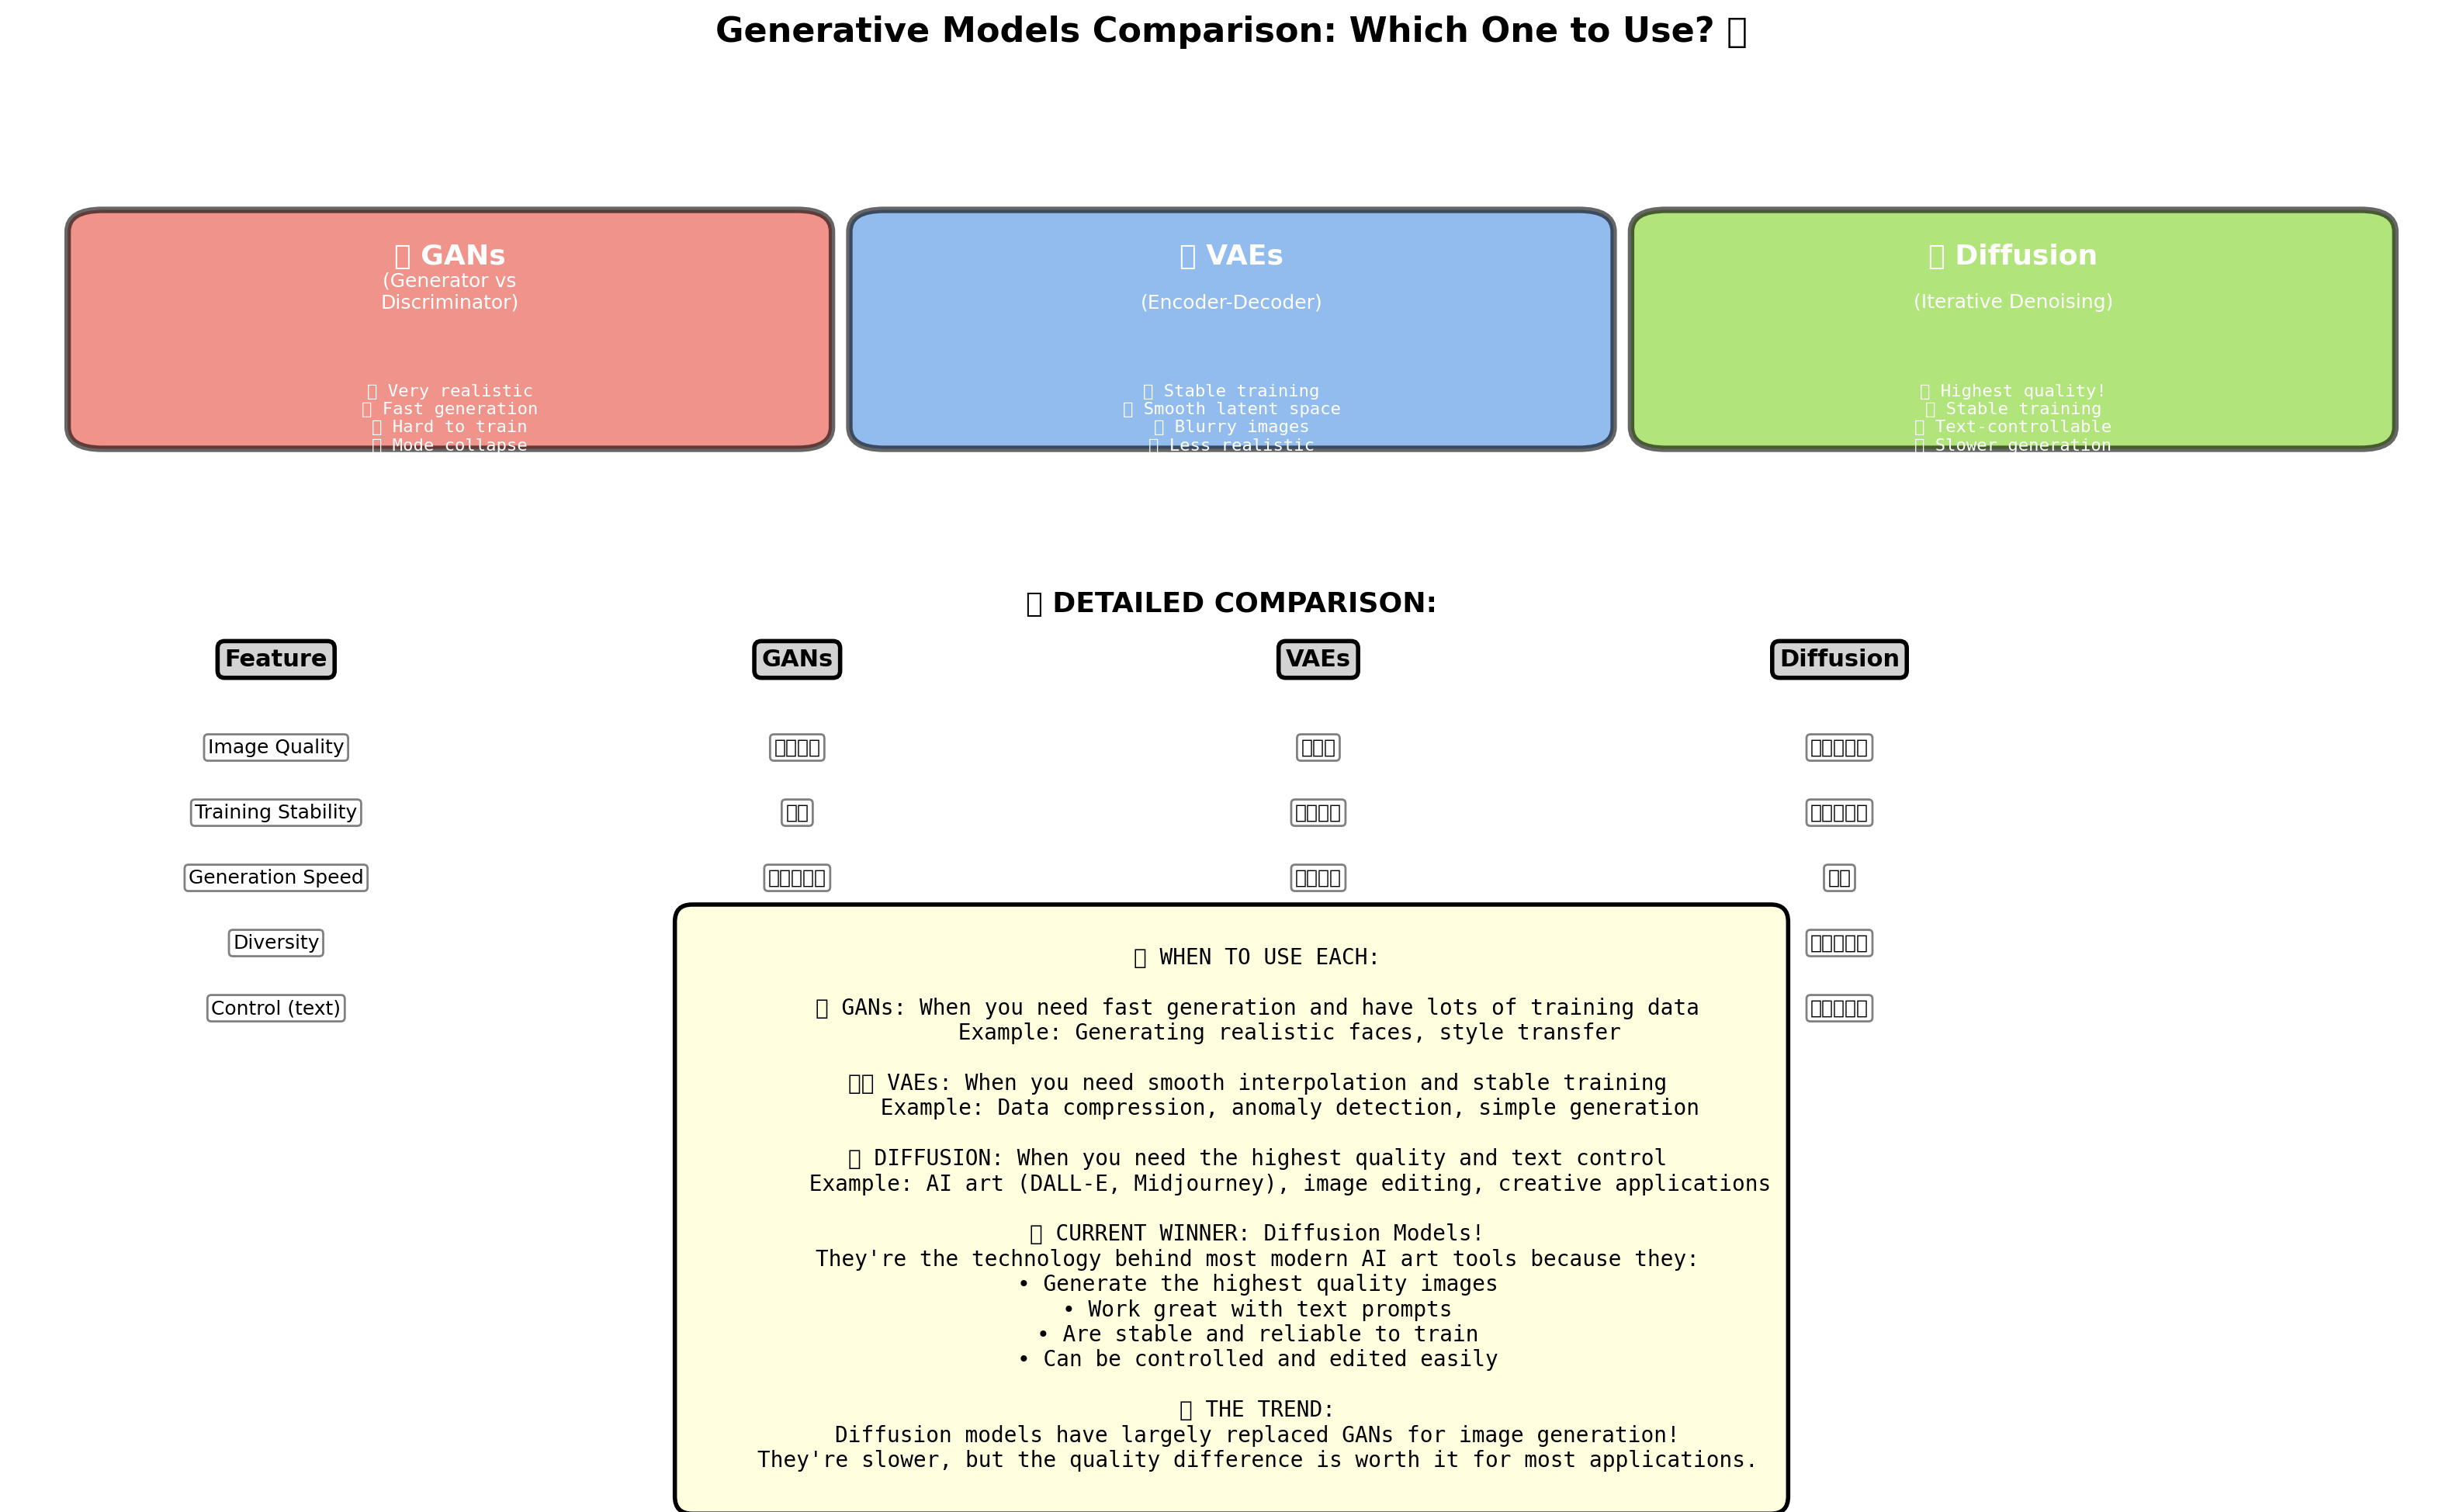
\includegraphics[width=0.85\textwidth]{../figures/diffusion_vs_others.png}

\vspace{0.2cm}

\begin{columns}[t]
\begin{column}{0.32\textwidth}
\begin{block}{GANs}
\textbf{Pros:} Fast generation\\
\textbf{Cons:} Hard to train, mode collapse
\end{block}
\end{column}

\begin{column}{0.32\textwidth}
\begin{block}{VAEs}
\textbf{Pros:} Stable, good latent space\\
\textbf{Cons:} Blurry outputs
\end{block}
\end{column}

\begin{column}{0.32\textwidth}
\begin{exampleblock}{Diffusion}
\textbf{Pros:} Best quality, stable\\
\textbf{Cons:} Slower generation
\end{exampleblock}
\end{column}
\end{columns}
\end{frame}

\begin{frame}{Diffusion Applications Overview}
\centering
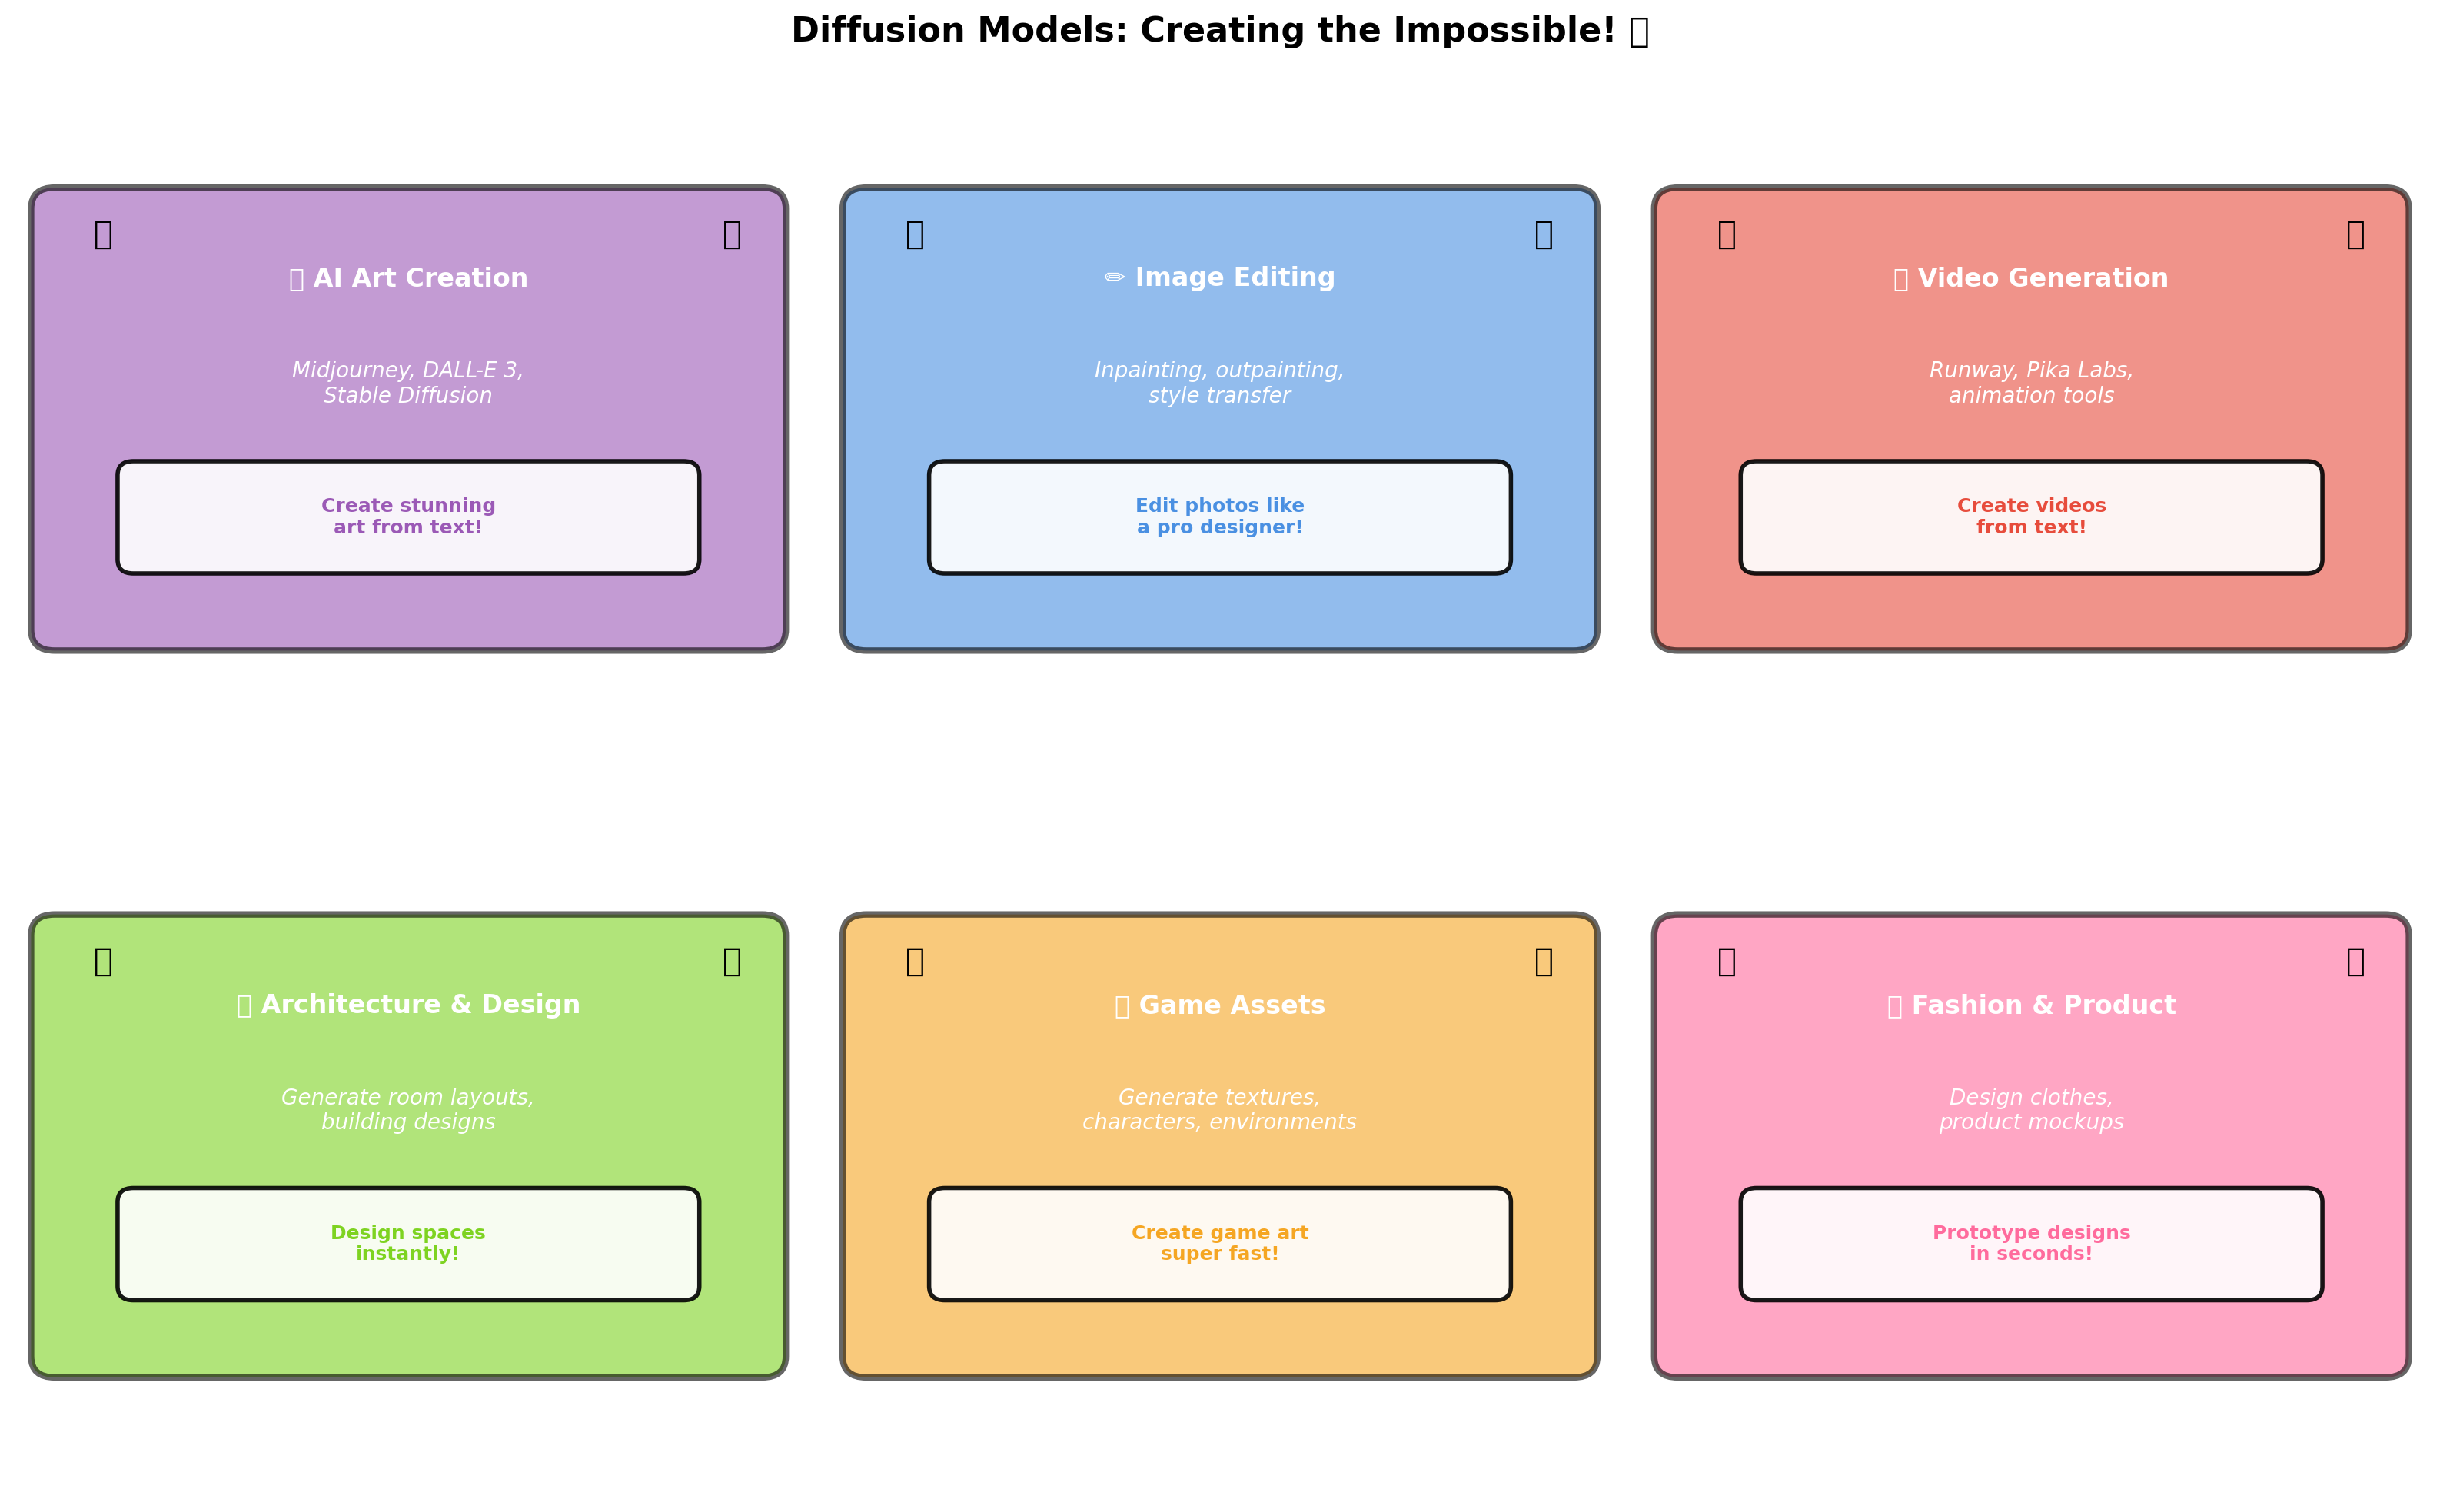
\includegraphics[width=0.88\textwidth]{../figures/diffusion_applications.png}

\vspace{0.2cm}

\begin{alertblock}{Why Diffusion Models Won}
They power DALL-E 2, Midjourney, Stable Diffusion - the best AI image generators today!
\end{alertblock}
\end{frame}

\begin{frame}{Diffusion Application: DALL-E 2}
\begin{columns}[t]
\begin{column}{0.48\textwidth}
\begin{block}{What DALL-E 2 Can Do}
\textbf{Text-to-Image Generation:}
\begin{itemize}
\setlength{\itemsep}{2pt}
\item Type a description, get an image
\item Photorealistic or artistic styles
\item Combine multiple concepts
\item Edit existing images
\item Outpainting (extend images)
\end{itemize}
\end{block}

\vspace{0.15cm}

\begin{exampleblock}{Example Prompts}
\begin{itemize}
\setlength{\itemsep}{2pt}
\item "A cat astronaut on Mars"
\item "Oil painting of a sunset over Manila"
\item "Teddy bear shopping for groceries"
\end{itemize}
\end{exampleblock}
\end{column}

\begin{column}{0.48\textwidth}
\begin{block}{Real-World Uses}
\begin{itemize}
\setlength{\itemsep}{2pt}
\item Marketing content creation
\item Concept art for entertainment
\item Educational illustrations
\item Social media graphics
\item Product mockups
\end{itemize}
\end{block}

\vspace{0.15cm}

\begin{alertblock}{By OpenAI}
Same company behind ChatGPT - 1.5+ million users create images daily!
\end{alertblock}
\end{column}
\end{columns}
\end{frame}

\begin{frame}{Diffusion Application: Midjourney}
\begin{columns}[t]
\begin{column}{0.48\textwidth}
\begin{block}{What Makes Midjourney Special}
\textbf{Artistic Focus:}
\begin{itemize}
\setlength{\itemsep}{2pt}
\item Exceptionally beautiful outputs
\item Strong artistic style
\item Great for fantasy/sci-fi art
\item Discord-based interface
\item Community of 16+ million users
\end{itemize}
\end{block}

\vspace{0.15cm}

\begin{exampleblock}{Popular Use Cases}
\begin{itemize}
\setlength{\itemsep}{2pt}
\item Book cover designs
\item Album artwork
\item Game concept art
\item NFT art generation
\end{itemize}
\end{exampleblock}
\end{column}

\begin{column}{0.48\textwidth}
\begin{block}{Industry Impact}
\begin{itemize}
\setlength{\itemsep}{2pt}
\item Artists use it for inspiration
\item Magazine covers created with AI
\item Award-winning art competitions
\item Commercial illustration work
\end{itemize}
\end{block}

\vspace{0.15cm}

\begin{alertblock}{Controversy}
AI art won Colorado State Fair - sparked debate about AI creativity!
\end{alertblock}
\end{column}
\end{columns}
\end{frame}

\begin{frame}{Diffusion Application: Stable Diffusion}
\begin{columns}[t]
\begin{column}{0.48\textwidth}
\begin{block}{Why Stable Diffusion is Different}
\textbf{Open Source:}
\begin{itemize}
\setlength{\itemsep}{2pt}
\item Free to use and modify
\item Run on your own computer
\item Customize and fine-tune
\item No usage restrictions
\item Active developer community
\end{itemize}
\end{block}

\vspace{0.15cm}

\begin{exampleblock}{Technical Details}
\begin{itemize}
\setlength{\itemsep}{2pt}
\item Can run on consumer GPUs
\item Faster than DALL-E 2
\item Extensible with plugins
\item Multiple versions and variants
\end{itemize}
\end{exampleblock}
\end{column}

\begin{column}{0.48\textwidth}
\begin{block}{Popular Applications Built With It}
\begin{itemize}
\setlength{\itemsep}{2pt}
\item DreamStudio (official interface)
\item Automatic1111 (popular UI)
\item ComfyUI (node-based editor)
\item Mobile apps (Draw Things)
\item Photoshop plugins
\end{itemize}
\end{block}

\vspace{0.15cm}

\begin{alertblock}{Democratizing AI}
Anyone with a decent computer can now generate professional-quality images!
\end{alertblock}
\end{column}
\end{columns}
\end{frame}

\begin{frame}{Diffusion Application: Adobe Firefly}
\begin{columns}[t]
\begin{column}{0.48\textwidth}
\begin{block}{Professional Image Editing}
\textbf{Firefly Features:}
\begin{itemize}
\setlength{\itemsep}{2pt}
\item Text-to-image generation
\item Generative fill (edit parts of images)
\item Text effects (3D text styles)
\item Generative recolor
\item Integrated in Photoshop
\end{itemize}
\end{block}

\vspace{0.15cm}

\begin{exampleblock}{Key Advantages}
\begin{itemize}
\setlength{\itemsep}{2pt}
\item Trained on Adobe Stock (licensed data)
\item Commercially safe to use
\item Professional quality outputs
\item Seamless Creative Cloud integration
\end{itemize}
\end{exampleblock}
\end{column}

\begin{column}{0.48\textwidth}
\begin{block}{Real Designer Workflows}
\begin{itemize}
\setlength{\itemsep}{2pt}
\item Remove unwanted objects
\item Extend backgrounds
\item Generate variations quickly
\item Create mockups from descriptions
\item Speed up creative process 10x
\end{itemize}
\end{block}

\vspace{0.15cm}

\begin{alertblock}{Industry Standard}
Adobe's AI tools are becoming essential for professional designers!
\end{alertblock}
\end{column}
\end{columns}
\end{frame}

\begin{frame}{Diffusion Application: Video Generation}
\begin{columns}[t]
\begin{column}{0.48\textwidth}
\begin{block}{Text-to-Video AI}
\textbf{Emerging Applications:}
\begin{itemize}
\setlength{\itemsep}{2pt}
\item Generate short video clips
\item Animate static images
\item Create transitions
\item Style transfer for video
\item AI-assisted editing
\end{itemize}
\end{block}

\vspace{0.15cm}

\begin{exampleblock}{Current Platforms}
\begin{itemize}
\setlength{\itemsep}{2pt}
\item \textbf{Runway Gen-2:} Text-to-video
\item \textbf{Pika Labs:} Video generation
\item \textbf{Stable Video Diffusion:} Open source
\end{itemize}
\end{exampleblock}
\end{column}

\begin{column}{0.48\textwidth}
\begin{block}{Use Cases}
\begin{itemize}
\setlength{\itemsep}{2pt}
\item Social media content
\item Marketing videos
\item Animated presentations
\item Film pre-visualization
\item Game cinematics
\end{itemize}
\end{block}

\vspace{0.15cm}

\begin{alertblock}{Future is Coming}
Video generation is improving rapidly - expect major breakthroughs soon!
\end{alertblock}
\end{column}
\end{columns}
\end{frame}

\begin{frame}{Text-to-Image Process Explained}
\centering
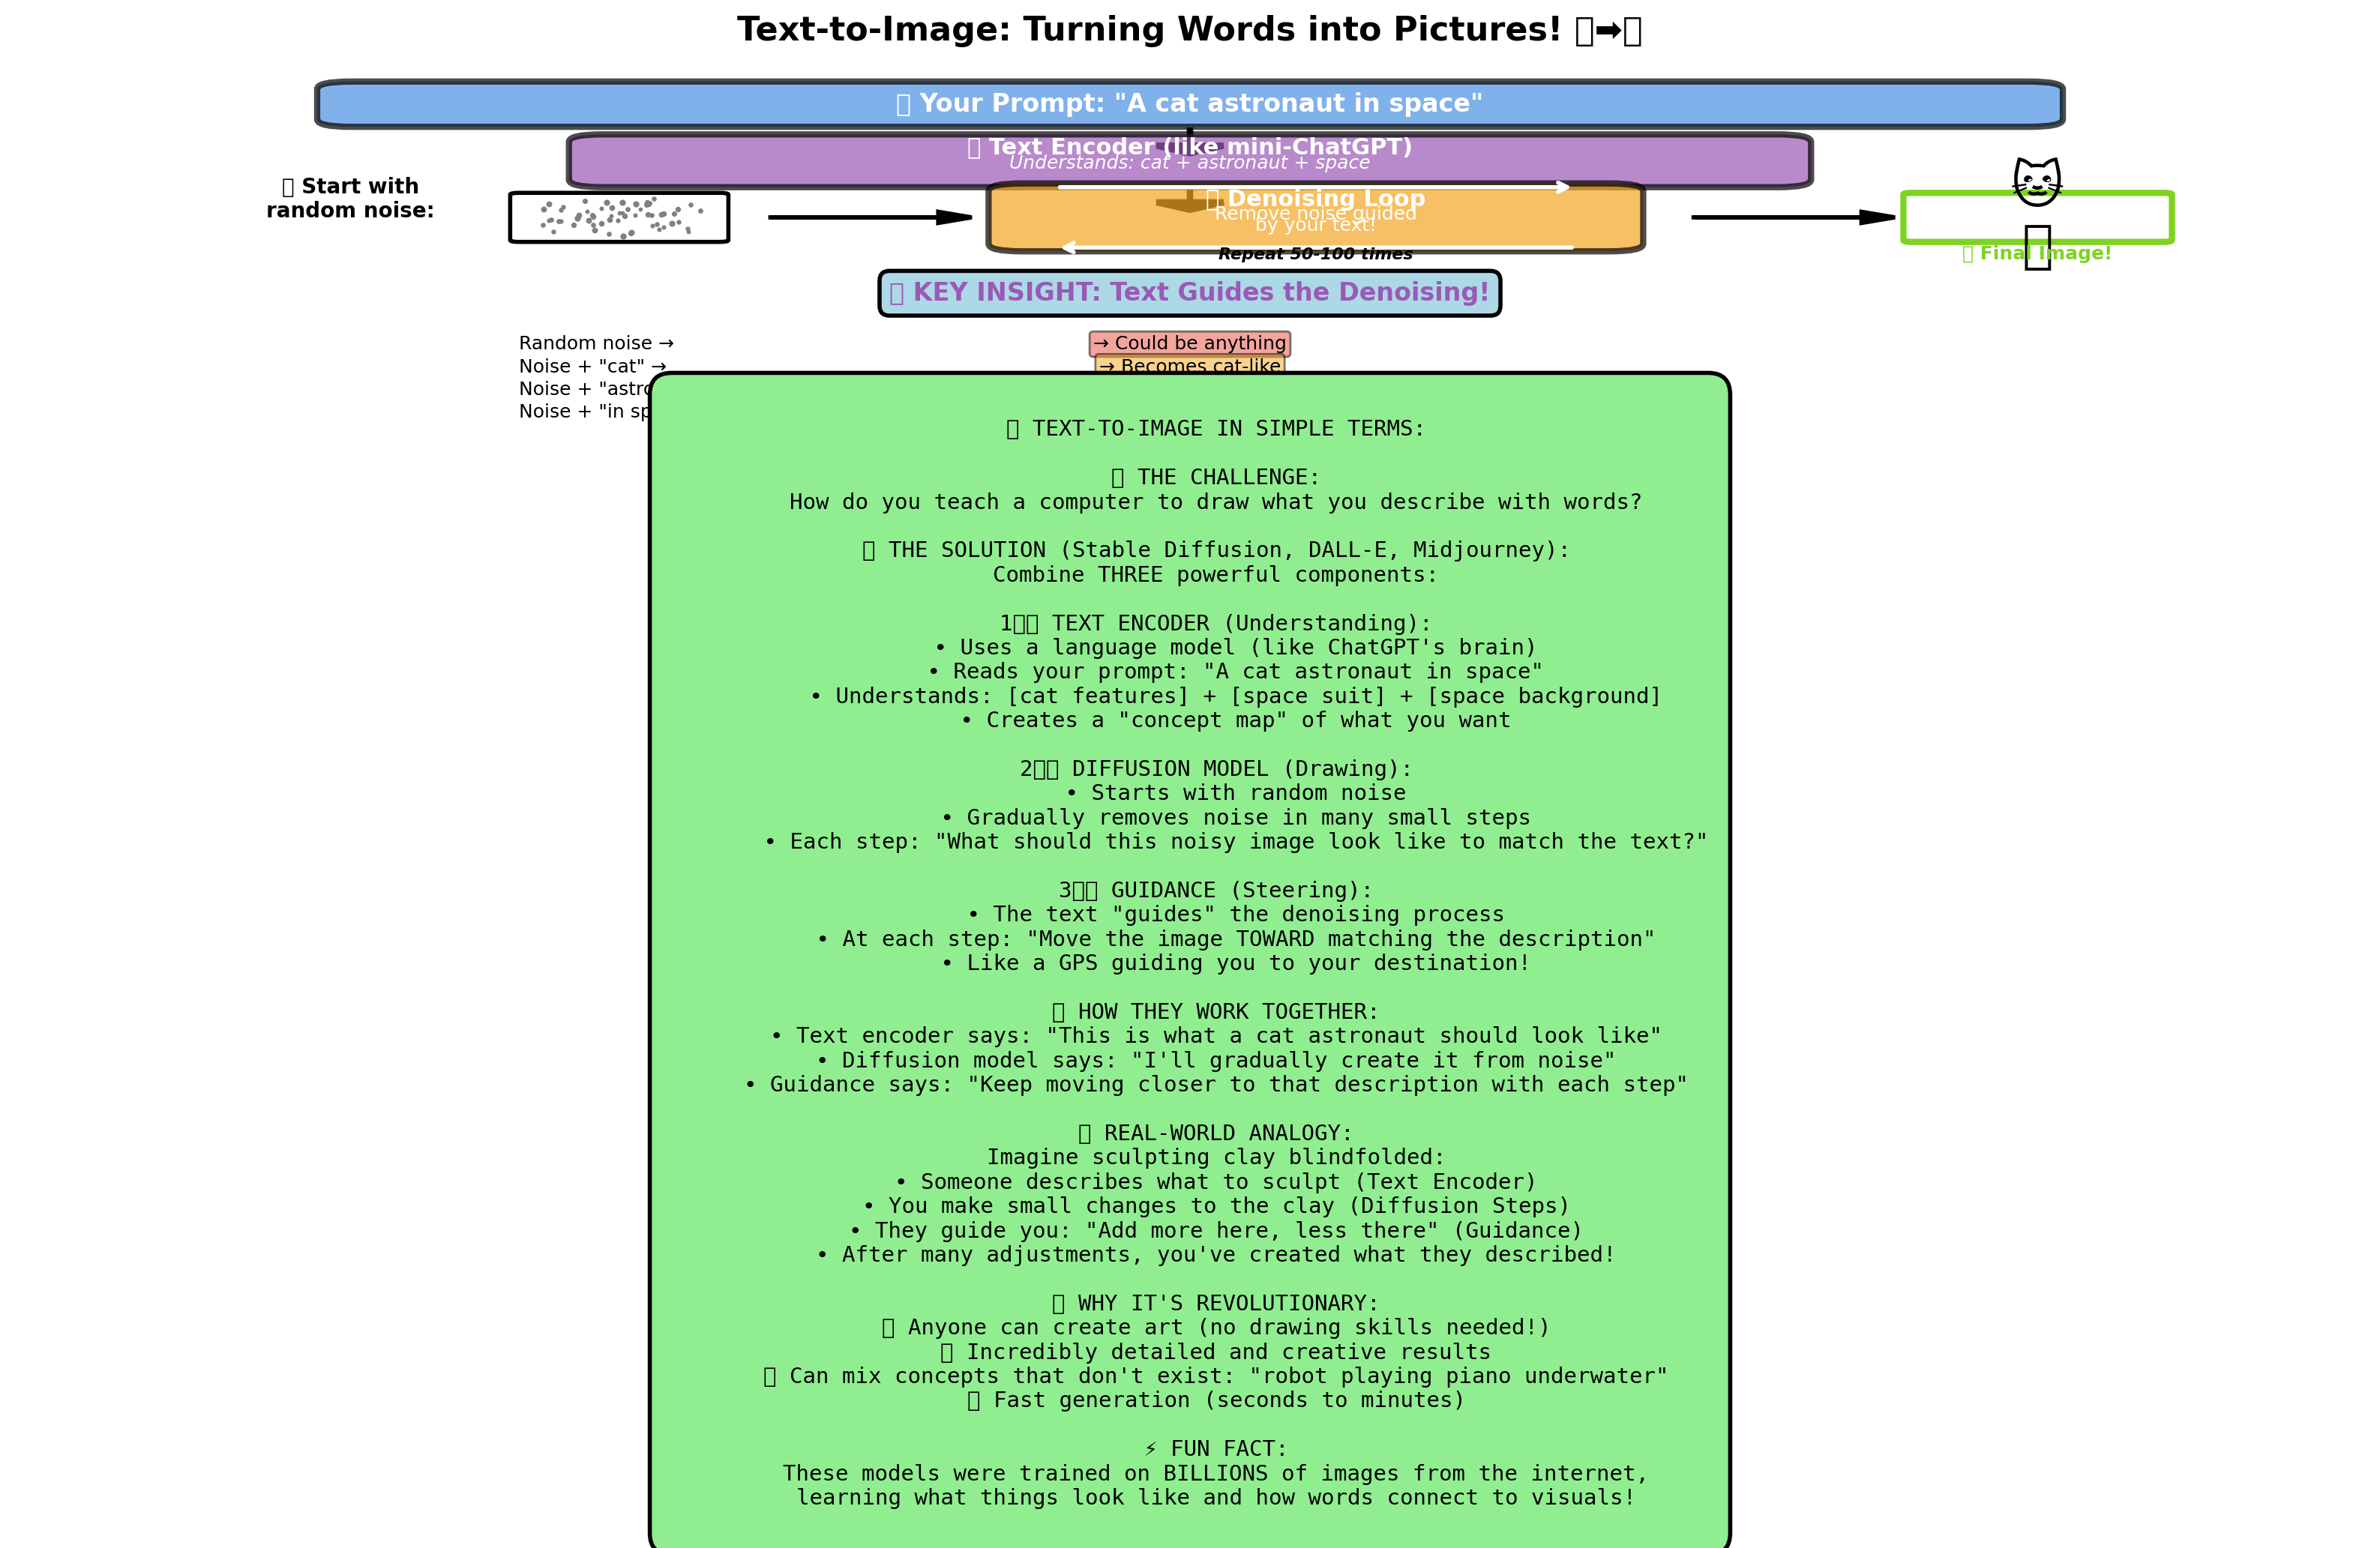
\includegraphics[width=0.88\textwidth]{../figures/text_to_image_process.png}

\vspace{0.2cm}

\begin{block}{How It All Works Together}
\begin{enumerate}
\setlength{\itemsep}{2pt}
\item \textbf{Text Encoder (Transformer):} Understand your description
\item \textbf{Diffusion Model:} Generate image from noise
\item \textbf{Guidance:} Steer generation toward text description
\item \textbf{Refinement:} Iteratively improve quality
\end{enumerate}
\end{block}
\end{frame}

% ========================================
% Section: Ethics and Considerations
% ========================================

\section{Ethics \& Responsible AI}

\begin{frame}{Ethical Considerations}
\centering
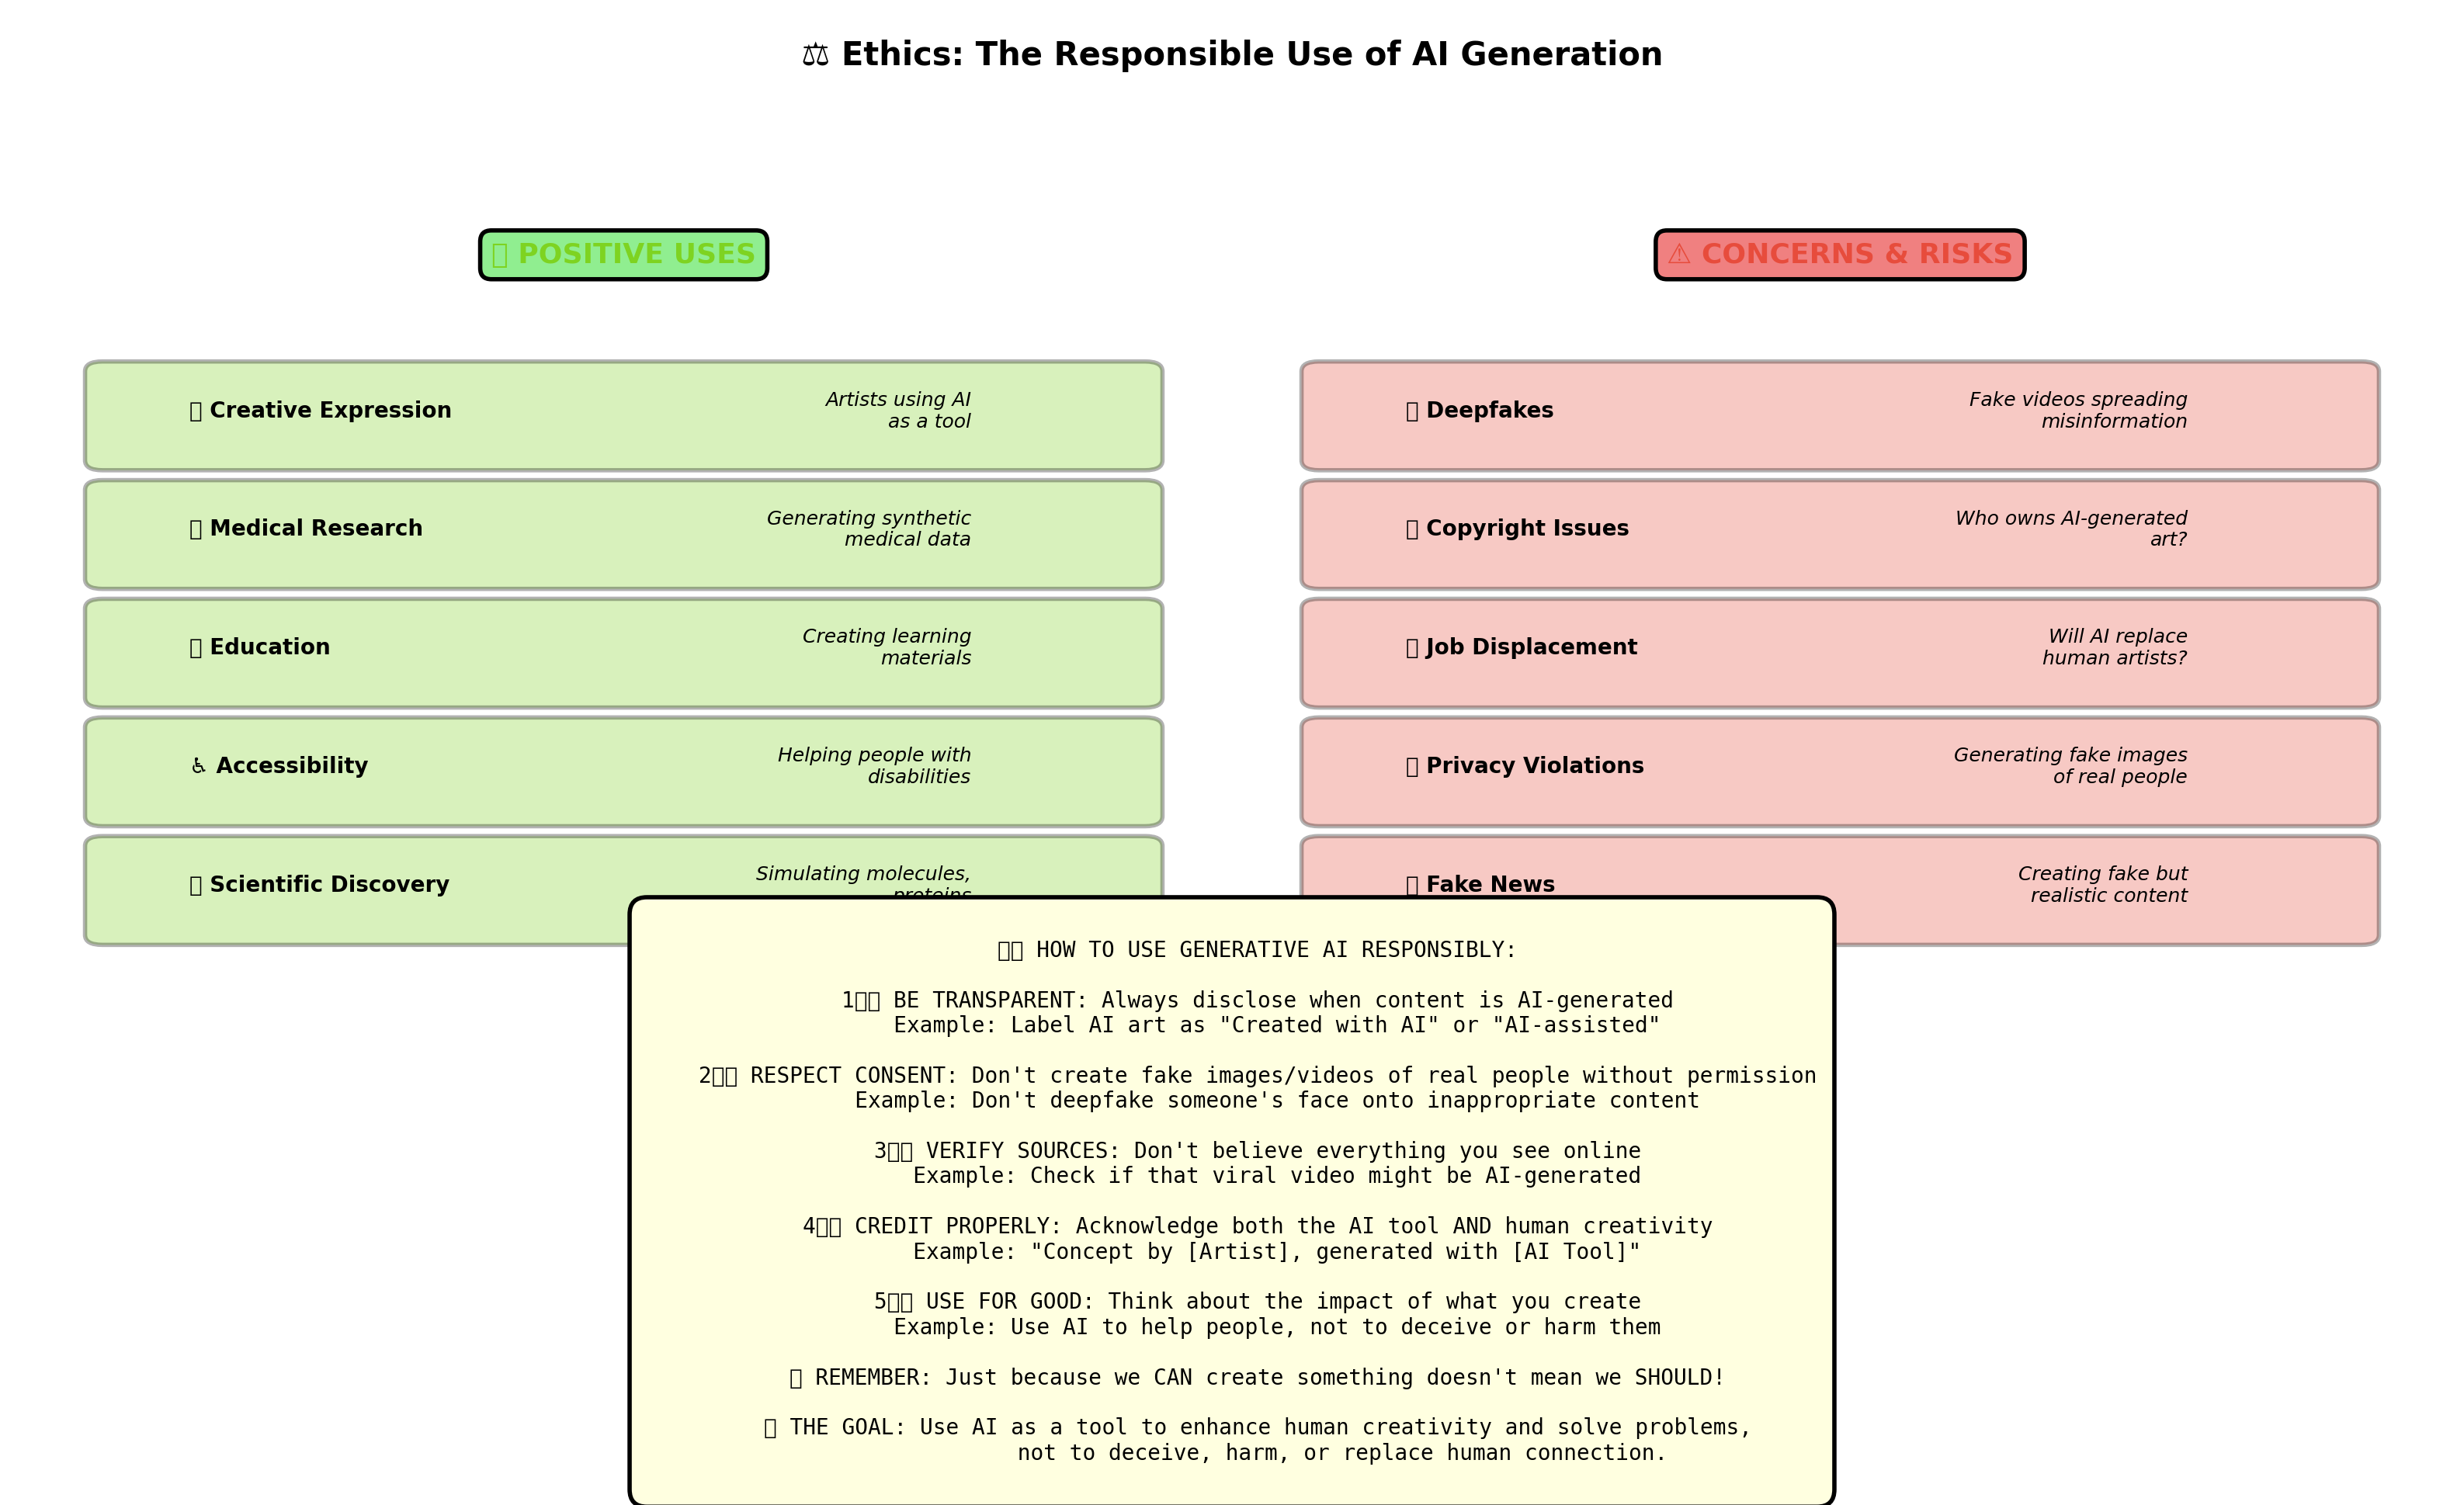
\includegraphics[width=0.85\textwidth]{../figures/generative_ethics.png}

\vspace{0.2cm}

\begin{alertblock}{Important Questions to Consider}
As these technologies become powerful, we must think carefully about their impact!
\end{alertblock}
\end{frame}

\begin{frame}{Key Ethical Issues}
\begin{columns}[t]
\begin{column}{0.48\textwidth}
\begin{block}{Misinformation \& Deepfakes}
\textbf{Concerns:}
\begin{itemize}
\setlength{\itemsep}{2pt}
\item Fake news and propaganda
\item Identity fraud
\item Non-consensual content
\item Erosion of trust in media
\end{itemize}

\vspace{0.1cm}

\textbf{Solutions:}
\begin{itemize}
\setlength{\itemsep}{2pt}
\item Detection technology
\item Digital watermarking
\item Media literacy education
\item Legal frameworks
\end{itemize}
\end{block}
\end{column}

\begin{column}{0.48\textwidth}
\begin{block}{Bias \& Fairness}
\textbf{Problems:}
\begin{itemize}
\setlength{\itemsep}{2pt}
\item Biased training data
\item Perpetuating stereotypes
\item Unfair representation
\item Discrimination in outputs
\end{itemize}

\vspace{0.1cm}

\textbf{Mitigation:}
\begin{itemize}
\setlength{\itemsep}{2pt}
\item Diverse training datasets
\item Bias testing and auditing
\item Responsible AI guidelines
\item Inclusive development teams
\end{itemize}
\end{block}
\end{column}
\end{columns}
\end{frame}

\begin{frame}{More Ethical Considerations}
\begin{columns}[t]
\begin{column}{0.48\textwidth}
\begin{block}{Copyright \& Intellectual Property}
\textbf{Questions:}
\begin{itemize}
\setlength{\itemsep}{2pt}
\item Who owns AI-generated content?
\item Is training on copyrighted data fair use?
\item Should artists be compensated?
\item How to attribute AI creations?
\end{itemize}

\vspace{0.1cm}

\textbf{Current Debates:}
\begin{itemize}
\setlength{\itemsep}{2pt}
\item Ongoing lawsuits (artists vs AI companies)
\item New legislation being proposed
\item Industry opt-out mechanisms
\end{itemize}
\end{block}
\end{column}

\begin{column}{0.48\textwidth}
\begin{block}{Job Displacement}
\textbf{Concerns:}
\begin{itemize}
\setlength{\itemsep}{2pt}
\item Will AI replace creative jobs?
\item Impact on artists, writers, designers
\item Economic inequality
\item Need for reskilling
\end{itemize}

\vspace{0.1cm}

\textbf{Opportunities:}
\begin{itemize}
\setlength{\itemsep}{2pt}
\item AI as a tool, not replacement
\item New creative possibilities
\item Democratization of creation
\item Focus on uniquely human skills
\end{itemize}
\end{block}
\end{column}
\end{columns}

\vspace{0.15cm}

\begin{alertblock}{Your Responsibility}
As future AI practitioners, think critically about the impact of your work!
\end{alertblock}
\end{frame}

% ========================================
% Section: Attention Mechanism
% ========================================

\section{Key Concept: Attention Mechanism}

\begin{frame}{Understanding Attention}
\centering
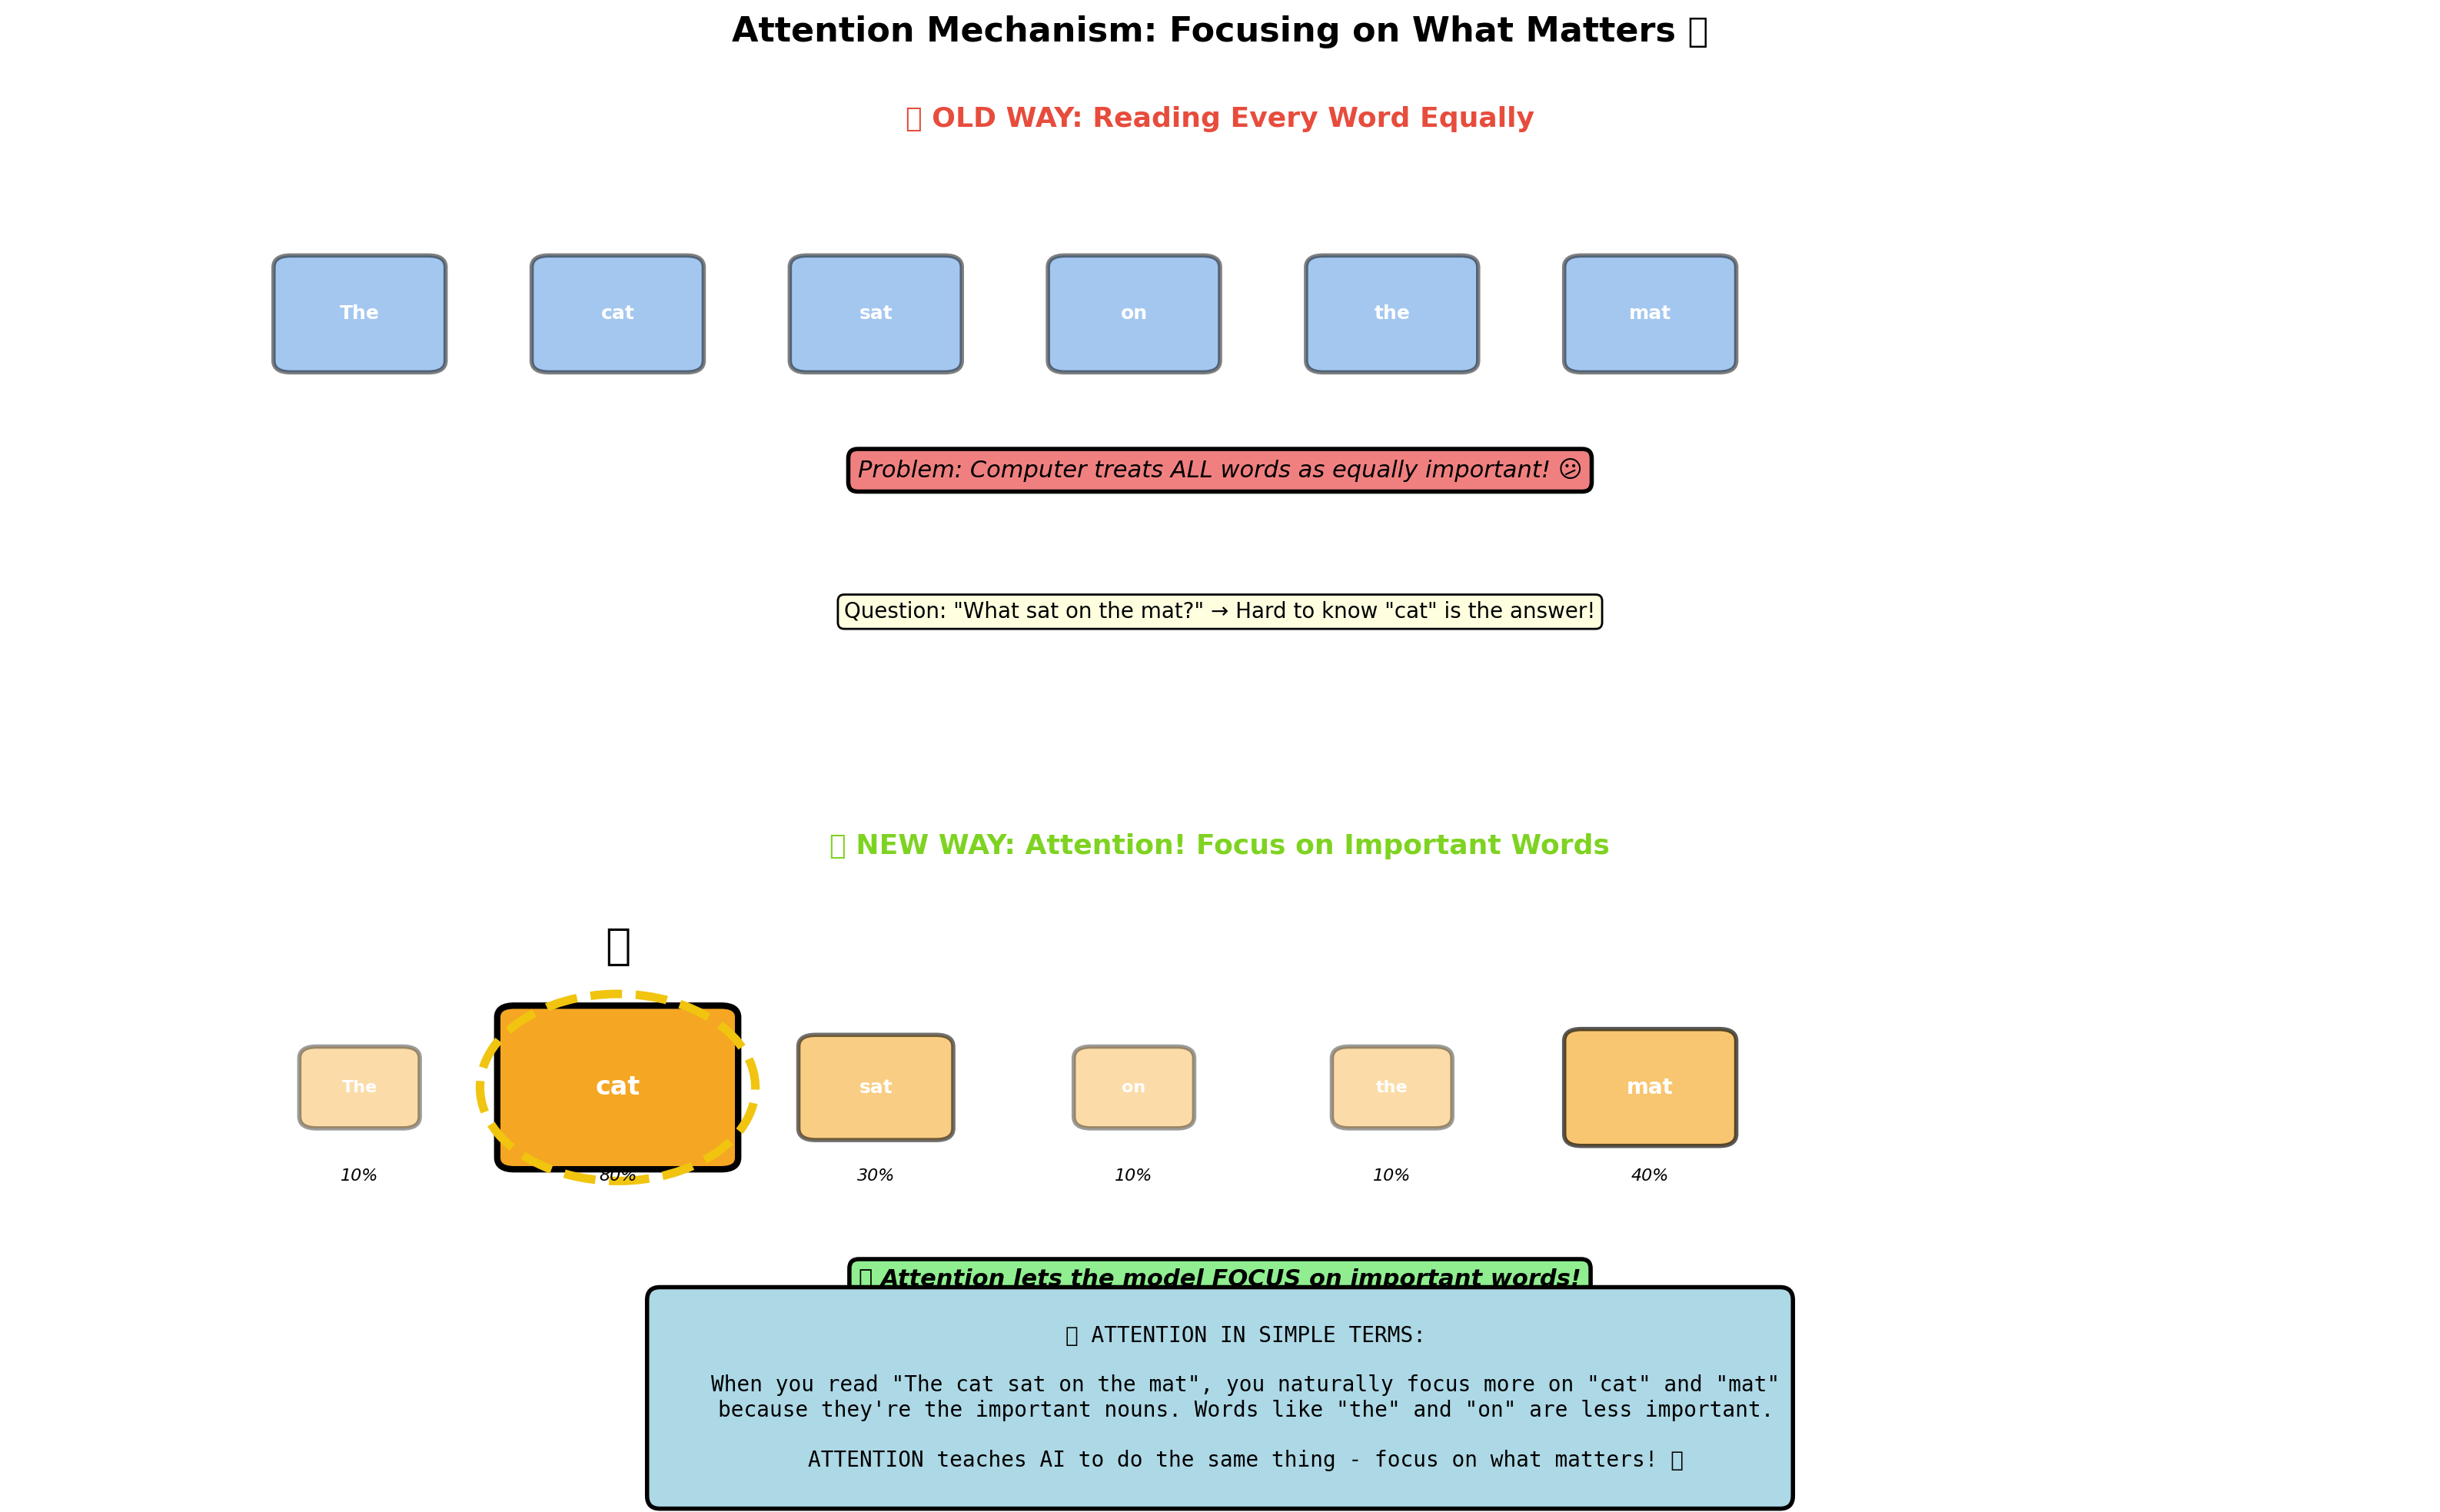
\includegraphics[width=0.85\textwidth]{../figures/attention_simple_concept.png}

\vspace{0.2cm}

\begin{block}{What is Attention?}
\textbf{A mechanism that lets neural networks focus on relevant parts:}
\begin{itemize}
\setlength{\itemsep}{3pt}
\item In text: Focus on important words in a sentence
\item In images: Focus on relevant image regions
\item Learns automatically what to pay attention to
\item Core component of Transformers
\end{itemize}
\end{block}
\end{frame}

\begin{frame}{Attention Example: Language Translation}
\begin{columns}[t]
\begin{column}{0.48\textwidth}
\begin{block}{Problem Without Attention}
\textbf{Translating: "The cat sat on the mat"}

Old approach:
\begin{itemize}
\setlength{\itemsep}{2pt}
\item Process word by word left to right
\item Forget earlier context
\item Struggle with long sentences
\item Poor word alignment
\end{itemize}
\end{block}
\end{column}

\begin{column}{0.48\textwidth}
\begin{exampleblock}{With Attention}
For each output word, the model:
\begin{itemize}
\setlength{\itemsep}{2pt}
\item Looks at ALL input words
\item Focuses on relevant ones
\item "sat" pays attention to "cat" and "mat"
\item Handles long-distance dependencies
\item Better translation quality
\end{itemize}
\end{exampleblock}
\end{column}
\end{columns}

\vspace{0.2cm}

\begin{alertblock}{Why It's Revolutionary}
Attention enabled Transformers to outperform all previous architectures!
\end{alertblock}
\end{frame}

% ========================================
% Section: Practical Tips
% ========================================

\section{Using These Models: Practical Guide}

\begin{frame}{Getting Started: Available Tools}
\begin{columns}[t]
\begin{column}{0.48\textwidth}
\begin{block}{Free/Accessible Tools}
\textbf{Try these today:}
\begin{itemize}
\setlength{\itemsep}{2pt}
\item \textbf{ChatGPT:} Free tier available
\item \textbf{Bing Image Creator:} Free DALL-E access
\item \textbf{Google Colab:} Run Stable Diffusion free
\item \textbf{Hugging Face:} Try many models online
\item \textbf{Runway:} Free trial for video
\end{itemize}
\end{block}

\vspace{0.15cm}

\begin{exampleblock}{Learning Resources}
\begin{itemize}
\setlength{\itemsep}{2pt}
\item Fast.ai courses (free)
\item Hugging Face tutorials
\item Papers with Code
\item YouTube: Two Minute Papers
\end{itemize}
\end{exampleblock}
\end{column}

\begin{column}{0.48\textwidth}
\begin{block}{For Developers}
\textbf{Build your own:}
\begin{itemize}
\setlength{\itemsep}{2pt}
\item PyTorch or TensorFlow
\item Hugging Face Transformers library
\item Stable Diffusion on GitHub
\item Pre-trained models available
\item Fine-tune on your data
\end{itemize}
\end{block}

\vspace{0.15cm}

\begin{alertblock}{Start Small}
Use existing models before building from scratch - learn by doing!
\end{alertblock}
\end{column}
\end{columns}
\end{frame}

\begin{frame}{Tips for Using AI Image Generators}
\begin{columns}[t]
\begin{column}{0.48\textwidth}
\begin{block}{Writing Good Prompts}
\textbf{Be specific:}
\begin{itemize}
\setlength{\itemsep}{2pt}
\item Describe style (photorealistic, cartoon, oil painting)
\item Specify details (colors, lighting, mood)
\item Mention composition (close-up, wide shot)
\item Add quality keywords (4K, detailed, masterpiece)
\end{itemize}
\end{block}

\vspace{0.1cm}

\begin{exampleblock}{Example Good Prompt}
"A majestic golden retriever sitting in a flower meadow at sunset, photorealistic, warm lighting, shallow depth of field, 4K quality"
\end{exampleblock}
\end{column}

\begin{column}{0.48\textwidth}
\begin{block}{Iteration is Key}
\begin{itemize}
\setlength{\itemsep}{2pt}
\item Generate multiple variations
\item Refine your prompt
\item Use negative prompts (what to avoid)
\item Adjust parameters (steps, guidance)
\item Learn from community prompts
\end{itemize}
\end{block}

\vspace{0.15cm}

\begin{alertblock}{Pro Tip}
Check out prompt libraries (Lexica.art, PromptHero) to learn from others!
\end{alertblock}
\end{column}
\end{columns}
\end{frame}

\begin{frame}{Common Challenges \& Solutions}
\begin{columns}[t]
\begin{column}{0.48\textwidth}
\begin{block}{Challenge: Poor Results}
\textbf{If outputs look bad:}
\begin{itemize}
\setlength{\itemsep}{2pt}
\item Improve your prompt specificity
\item Try different seed values
\item Adjust generation parameters
\item Use a different model/variant
\item Increase generation steps
\end{itemize}
\end{block}

\vspace{0.1cm}

\begin{block}{Challenge: Wrong Anatomy/Details}
\textbf{Known limitations:}
\begin{itemize}
\setlength{\itemsep}{2pt}
\item Hands and fingers often wrong
\item Text in images unclear
\item Physics may be incorrect
\item Use inpainting to fix specific parts
\end{itemize}
\end{block}
\end{column}

\begin{column}{0.48\textwidth}
\begin{block}{Challenge: Slow Generation}
\textbf{Speed up:}
\begin{itemize}
\setlength{\itemsep}{2pt}
\item Use lower resolution first
\item Reduce number of steps
\item Try faster samplers
\item Use GPU acceleration
\item Consider paid services for speed
\end{itemize}
\end{block}

\vspace{0.1cm}

\begin{block}{Challenge: Reproducibility}
\textbf{Get consistent results:}
\begin{itemize}
\setlength{\itemsep}{2pt}
\item Save your seed numbers
\item Keep prompt exactly the same
\item Note all parameters used
\item Use img2img for variations
\end{itemize}
\end{block}
\end{column}
\end{columns}
\end{frame}

% ========================================
% Section: Summary
% ========================================

\section{Summary \& Looking Forward}

\begin{frame}{Key Takeaways}
\begin{block}{What We Learned}
\textbf{Five major architectures changing the world:}
\begin{enumerate}
\setlength{\itemsep}{3pt}
\item \textbf{CNNs:} Revolutionized computer vision (medical imaging, self-driving cars, face recognition)
\item \textbf{GANs:} Generate realistic images (AI art, deepfakes, synthetic data)
\item \textbf{VAEs:} Compress and generate (anomaly detection, drug discovery)
\item \textbf{Transformers:} Dominated NLP (ChatGPT, translation, code generation)
\item \textbf{Diffusion:} Best image generation (DALL-E 2, Midjourney, Stable Diffusion)
\end{enumerate}
\end{block}

\vspace{0.15cm}

\begin{alertblock}{Main Message}
These aren't just research projects - they're tools you can use TODAY in real applications!
\end{alertblock}
\end{frame}

\begin{frame}{Applications Summary}
\begin{columns}[t]
\begin{column}{0.48\textwidth}
\begin{block}{CNNs Applications}
\begin{itemize}
\setlength{\itemsep}{2pt}
\item Medical tumor detection
\item Self-driving lane detection
\item Phone face unlock
\item Security cameras
\item Satellite imagery analysis
\end{itemize}
\end{block}

\vspace{0.1cm}

\begin{block}{GAN Applications}
\begin{itemize}
\setlength{\itemsep}{2pt}
\item Artbreeder AI art
\item Deepfake detection
\item Synthetic medical data
\item Game character creation
\item Fashion design
\end{itemize}
\end{block}
\end{column}

\begin{column}{0.48\textwidth}
\begin{block}{Transformer Applications}
\begin{itemize}
\setlength{\itemsep}{2pt}
\item ChatGPT conversations
\item Google Translate
\item GitHub Copilot
\item Email auto-complete
\item Document summarization
\end{itemize}
\end{block}

\vspace{0.1cm}

\begin{block}{Diffusion Applications}
\begin{itemize}
\setlength{\itemsep}{2pt}
\item DALL-E 2 image generation
\item Midjourney art creation
\item Stable Diffusion (open source)
\item Adobe Firefly editing
\item Video generation (emerging)
\end{itemize}
\end{block}
\end{column}
\end{columns}
\end{frame}

\begin{frame}{The Future is Here}
\begin{columns}[t]
\begin{column}{0.48\textwidth}
\begin{block}{Trends to Watch}
\textbf{Next 1-2 years:}
\begin{itemize}
\setlength{\itemsep}{2pt}
\item \textbf{Multimodal AI:} Text, image, audio, video together
\item \textbf{Better video generation:} Movie-quality AI videos
\item \textbf{3D generation:} Create 3D models from text
\item \textbf{Real-time generation:} Instant results
\item \textbf{Personalization:} AI that learns your style
\end{itemize}
\end{block}
\end{column}

\begin{column}{0.48\textwidth}
\begin{exampleblock}{Career Opportunities}
\textbf{Skills in demand:}
\begin{itemize}
\setlength{\itemsep}{2pt}
\item AI/ML engineering
\item Prompt engineering
\item AI safety and ethics
\item Creative AI applications
\item AI product management
\end{itemize}
\end{exampleblock}

\vspace{0.15cm}

\begin{alertblock}{Get Involved}
The best way to learn is to experiment - start building today!
\end{alertblock}
\end{column}
\end{columns}
\end{frame}

\begin{frame}{How to Continue Learning}
\begin{columns}[t]
\begin{column}{0.48\textwidth}
\begin{block}{Hands-On Practice}
\begin{itemize}
\setlength{\itemsep}{2pt}
\item Try Stable Diffusion on Colab
\item Build projects with Hugging Face
\item Fine-tune models on your data
\item Participate in Kaggle competitions
\item Contribute to open source projects
\end{itemize}
\end{block}

\vspace{0.15cm}

\begin{block}{Online Courses}
\begin{itemize}
\setlength{\itemsep}{2pt}
\item Fast.ai: Practical Deep Learning
\item Stanford CS230: Deep Learning
\item Coursera: Deep Learning Specialization
\item Hugging Face NLP Course (free)
\end{itemize}
\end{block}
\end{column}

\begin{column}{0.48\textwidth}
\begin{block}{Stay Updated}
\begin{itemize}
\setlength{\itemsep}{2pt}
\item Follow Papers with Code
\item Read AI newsletters (The Batch, etc.)
\item Watch Two Minute Papers (YouTube)
\item Join AI Discord communities
\item Attend local meetups
\end{itemize}
\end{block}

\vspace{0.15cm}

\begin{exampleblock}{Next Steps in This Course}
\textbf{Workshop:} Hands-on coding with ResNet, GPT-2, Stable Diffusion - let's use these models!
\end{exampleblock}
\end{column}
\end{columns}
\end{frame}

\begin{frame}{Questions?}
\centering
\vspace{1cm}

{\Large\textbf{Thank you for your attention!}}

\vspace{1cm}

\begin{block}{Contact Information}
\textbf{Instructor:} Noel Jeffrey Pinton\\
\textbf{Course:} CMSC 173 - Machine Learning\\
\textbf{Institution:} University of the Philippines - Cebu\\
\textbf{Department:} Computer Science
\end{block}

\vspace{0.5cm}

\begin{alertblock}{Remember}
Advanced neural networks are tools that empower creativity and solve real problems. Use them responsibly and ethically!
\end{alertblock}
\end{frame}

\end{document}
